% Seminar: Recapitulare
% Statistica Piețelor Financiare

\documentclass[9pt, aspectratio=169, t]{beamer}
%=============================================================================
% PREAMBUL COMUN - Statistica Piețelor Financiare
% Versiune robustă pentru macOS (MacTeX / BasicTeX / TeX Live)
% Daniel Traian Pele, Antoaneta Amza - ASE București
%
% MODIFICĂRI față de varianta originală:
%  (1) fontawesome5 făcut OPȚIONAL (\IfFileExists) → nu mai pică dacă lipsește
%  (2) polyglossia cu fallback automat pe babel dacă romanian nu există
%  (3) setmainfont rescris cu Ligatures=TeX și nume normalizate (merge pe macOS)
%  (4) graphicspath extins (include directorul curent + variante relative) ca
%      logo-urile să fie găsite și când lansezi xelatex dintr-un subdirector
%
% Compilare:  xelatex preamble + main, de DOUĂ ori (toc/ref).
%=============================================================================

% Asigură încadrarea conținutului pe diapozitive
\setbeamersize{text margin left=8mm, text margin right=8mm}

%=============================================================================
% CONFIGURARE TEMĂ ȘI STIL
%=============================================================================
\usetheme{default}

% Paletă de Culori
\definecolor{MainBlue}{RGB}{26, 58, 110}
\definecolor{AccentBlue}{RGB}{26, 58, 110}
\definecolor{IDAred}{RGB}{205, 0, 0}
\definecolor{DarkGray}{RGB}{51, 51, 51}
\definecolor{MediumGray}{RGB}{128, 128, 128}
\definecolor{LightGray}{RGB}{248, 248, 248}
\definecolor{VeryLightGray}{RGB}{235, 235, 235}
\definecolor{KeynoteGray}{RGB}{218, 218, 218}
\definecolor{SectionGray}{RGB}{120, 120, 120}
\definecolor{FooterGray}{RGB}{100, 100, 100}
\definecolor{Crimson}{RGB}{220, 53, 69}
\definecolor{Forest}{RGB}{46, 125, 50}
\definecolor{Amber}{RGB}{181, 133, 63}
\definecolor{Orange}{RGB}{230, 126, 34}
\definecolor{Purple}{RGB}{142, 68, 173}

% Fundal gradient (gradient Keynote exact 315°: alb la RGB 218,218,218)
\setbeamertemplate{background}{%
	\begin{tikzpicture}[remember picture, overlay]
		\shade[shading=axis, shading angle=315,
		top color=white, bottom color=KeynoteGray]
		(current page.south west) rectangle (current page.north east);
	\end{tikzpicture}%
}
% Culoare solidă de rezervă pentru compatibilitate
\setbeamercolor{background canvas}{bg=}

\setbeamercolor{palette primary}{bg=MainBlue, fg=white}
\setbeamercolor{palette secondary}{bg=MainBlue!85, fg=white}
\setbeamercolor{palette tertiary}{bg=MainBlue!70, fg=white}
\setbeamercolor{structure}{fg=MainBlue}
\setbeamercolor{title}{fg=IDAred}
\setbeamercolor{frametitle}{fg=IDAred, bg=}
\setbeamercolor{block title}{bg=MainBlue, fg=white}
\setbeamercolor{block body}{bg=VeryLightGray, fg=DarkGray}
\setbeamercolor{block title alerted}{bg=Crimson, fg=white}
\setbeamercolor{block body alerted}{bg=Crimson!8, fg=DarkGray}
\setbeamercolor{block title example}{bg=Forest, fg=white}
\setbeamercolor{block body example}{bg=Forest!8, fg=DarkGray}
\setbeamercolor{item}{fg=MainBlue}

\setbeamerfont{institute}{size=\footnotesize}

\setbeamercolor{author in head/foot}{fg=FooterGray, bg=}
\setbeamercolor{title in head/foot}{fg=FooterGray, bg=}
\setbeamercolor{date in head/foot}{fg=FooterGray, bg=}
\setbeamercolor{section in head/foot}{fg=FooterGray, bg=}
\setbeamercolor{subsection in head/foot}{fg=FooterGray, bg=}

\setbeamertemplate{itemize item}{\color{MainBlue}$\boxdot$}
\setbeamertemplate{itemize subitem}{\color{MainBlue}$\blacktriangleright$}
\setbeamertemplate{itemize subsubitem}{\color{MainBlue}\tiny$\bullet$}
\setbeamertemplate{itemize/enumerate body begin}{\normalsize}
\setbeamertemplate{itemize/enumerate subbody begin}{\normalsize}

\setbeamertemplate{section in toc}{%
	\leavevmode\leftskip=1.5em%
	\llap{\color{MainBlue}$\boxdot$\kern0.5em}%
	\inserttocsection\par%
}

\setlength{\leftmargini}{10pt}
\setlength{\leftmarginii}{10pt}
\makeatletter
\def\@listi{\leftmargin\leftmargini \topsep 0pt \parsep 0pt \itemsep 0pt}
\def\@listii{\leftmargin\leftmarginii \topsep 0pt \parsep 0pt \itemsep 0pt}
\makeatother

\setbeamertemplate{navigation symbols}{}

%=============================================================================
% ANTET PERSONALIZAT
%=============================================================================
\setbeamertemplate{headline}{%
	\vskip10pt%
	\hbox to \paperwidth{%
		\hskip0.5cm%
		{\small\color{FooterGray}\renewcommand{\hyperlink}[2]{##2}\insertsectionhead}%
		\hfill%
		\textcolor{FooterGray}{\small\insertframenumber}%
		\hskip0.5cm%
	}%
	\vskip4pt%
	{\color{FooterGray}\hrule height 0.4pt}%
}

%=============================================================================
% PACHETE — ordine importantă: fontspec ÎNAINTE de polyglossia/babel
%=============================================================================

% --- (1) FONTSPEC + FONTURI ROBUSTE PE macOS ---
\usepackage{fontspec}
% Pe macOS unele fonturi Latin Modern nu sunt înregistrate ca fonturi de sistem.
% Folosim Ligatures=TeX (pentru -- → en-dash etc.) și lăsăm fontspec să caute
% prin kpathsea (merge atât pe Mac, cât și pe Linux/Windows).
\defaultfontfeatures{Ligatures=TeX}
\IfFontExistsTF{Latin Modern Roman}{%
	\setmainfont{Latin Modern Roman}
	\setsansfont{Latin Modern Sans}
	\setmonofont{Latin Modern Mono}
}{%
	% Fallback dacă numele cu spații nu sunt găsite (cazul macOS fără fonturi
	% Latin Modern în /Library/Fonts) — fontspec va folosi fontul implicit.
	\PackageWarning{preamble}{Latin Modern Roman nu a fost gasit; folosesc fontul implicit.}
}

% --- (2) POLYGLOSSIA SAU BABEL CU FALLBACK ---
% Pe versiuni vechi de polyglossia (TeX Live < 2020) limba `romanian` nu există.
% Detectăm și folosim babel ca rezervă.
\IfFileExists{gloss-romanian.ldf}{%
	\usepackage{polyglossia}
	\setdefaultlanguage{romanian}
	\setotherlanguage{english}
}{%
	\PackageWarning{preamble}{polyglossia/romanian indisponibil; folosesc babel.}
	\usepackage[english,romanian]{babel}
}

% --- (3) MATH ȘI GRAFICĂ ---
\usepackage{amsmath, amssymb, amsthm}
\usepackage{mathtools}
\usepackage{bm}
\usepackage{tikz}
\usetikzlibrary{arrows.meta, positioning, shapes, calc, decorations.pathreplacing, shadings}
\usepackage{booktabs}
\usepackage{multirow}
\usepackage{array}
\usepackage{graphicx}
\usepackage{hyperref}
\usepackage{colortbl}
\usepackage{listings}
\lstset{basicstyle=\ttfamily\small, breaklines=true, frame=single, backgroundcolor=\color{VeryLightGray}}
\hypersetup{colorlinks=true, linkcolor=MainBlue, urlcolor=MainBlue}

% --- (4) GRAPHICSPATH cu directorul curent inclus ca fallback ---
\graphicspath{{./}{./logos/}{./charts/}{./photos/}{../logos/}{../charts/}{../photos/}{../../logos/}{../../charts/}{../../photos/}}
\hfuzz=2pt
\vfuzz=2pt

%=============================================================================
% SUBSOL PERSONALIZAT — fontawesome5 făcut OPȚIONAL
%=============================================================================
% Pe BasicTeX / instalări minime de MacTeX, fontawesome5 nu există.
% Dacă lipsește, omitem icoanele (subsolul rămâne curat).
\IfFileExists{fontawesome5.sty}{%
	\usepackage{fontawesome5}
	\newcommand{\hasfontawesome}{true}
}{%
	\PackageWarning{preamble}{fontawesome5 indisponibil; subsolul nu va contine icoane.}
}

\setbeamertemplate{footline}{%
	{\color{FooterGray}\hrule height 0.4pt}%
	\vskip4pt%
	\hbox to \paperwidth{%
		\hskip0.5cm%
		\textcolor{FooterGray}{\small Statistica Piețelor Financiare}%
		\hfill%
		\raisebox{-0.1em}{%
			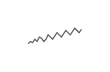
\begin{tikzpicture}[x=0.08em, y=0.08em, line width=0.4pt]
				\draw[FooterGray] (0,3) -- (1,4) -- (2,3.5) -- (3,5) -- (4,4) -- (5,6) -- (6,5.5) -- (7,4) -- (8,5) -- (9,7) -- (10,6) -- (11,5) -- (12,6.5) -- (13,8) -- (14,7) -- (15,6) -- (16,7.5) -- (17,9) -- (18,8) -- (19,7) -- (20,8.5) -- (21,10) -- (22,9) -- (23,8) -- (24,9.5);
			\end{tikzpicture}%
		}%
		\hskip0.5cm%
	}%
	\vskip6pt%
}

%=============================================================================
% COMANDA QUANTLET
%=============================================================================
\newcommand{\quantlet}[2]{%
	\hfill\href{#2}{%
		\raisebox{-0.15em}{
\includegraphics[height=0.7em]{ql_logo.png}}%
		\textcolor{MainBlue}{\tiny\ #1}%
	}%
}

%=============================================================================
% PAGINĂ TITLU PERSONALIZATĂ
%=============================================================================
\defbeamertemplate*{title page}{hybrid}[1][]
{
	\vspace{0.2cm}
	\noindent\makebox[\linewidth][s]{%
		\href{https://www.ase.ro}{
\includegraphics[height=1.0cm]{ase_logo.png}}\hfill%
		\href{https://theida.net}{
\includegraphics[height=1.0cm]{ida_logo.png}}\hfill%
		\href{https://blockchain-research-center.com}{
\includegraphics[height=1.0cm]{brc_logo.png}}\hfill%
		\href{https://www.ai4efin.ase.ro}{
\includegraphics[height=1.0cm]{ai4efin_logo.png}}\hfill%
		\href{https://ipe.ro/new}{
\includegraphics[height=1.0cm]{acad_logo.png}}\hfill%
		\href{https://www.digital-finance-msca.com}{
\includegraphics[height=1.0cm]{msca_logo.png}}%
	}
	\vspace{0.6cm}
	
	\noindent\makebox[\linewidth][c]{%
		\begin{minipage}{0.11\linewidth}
			\centering
			\href{https://quantlet.com}{
\includegraphics[height=1.1cm]{ql_logo.png}}
		\end{minipage}%
		\begin{minipage}{0.76\linewidth}
			\centering
			{\LARGE\bfseries\usebeamercolor[fg]{title}\inserttitle}
			
			\vspace{0.3cm}
			
			{\usebeamerfont{subtitle}\usebeamercolor[fg]{title}\insertsubtitle}
		\end{minipage}%
		\begin{minipage}{0.11\linewidth}
			\centering
			\href{https://quantinar.com}{
\includegraphics[height=1.1cm]{qr_logo.png}}
		\end{minipage}%
	}
	
	\vspace{0.6cm}
	
	\hspace{0.5cm}{\usebeamerfont{author}\insertauthor}
	
	\vspace{0.3cm}
	
	\hspace{0.5cm}\begin{minipage}[t]{0.9\textwidth}
		\raggedright\small\insertinstitute
	\end{minipage}
}
\setbeamertemplate{title page}[hybrid]

%=============================================================================
% MEDII PENTRU TEOREME
%=============================================================================
\theoremstyle{definition}
\setbeamertemplate{theorems}[numbered]
\newtheorem{defn}{Definiție}
\newtheorem{thm}{Teoremă}
\newtheorem{prop}{Propoziție}
\newtheorem{rmk}{Observație}

%=============================================================================
% CENTRED MINIPAGE
%=============================================================================
\newenvironment{cminipage}[1]{%
	\par\noindent\hfill\begin{minipage}{#1}\ignorespaces
	}{%
	\end{minipage}\hfill\null\par
}

%=============================================================================
% COMENZI PERSONALIZATE
%=============================================================================
\newcommand{\E}{\mathbb{E}}
\newcommand{\Var}{\text{Var}}
\newcommand{\Cov}{\text{Cov}}
\newcommand{\Corr}{\text{Corr}}
\newcommand{\VaR}{\text{VaR}}
\newcommand{\ES}{\text{ES}}
\newcommand{\R}{\mathbb{R}}
\newcommand{\N}{\mathbb{N}}
\newcommand{\Z}{\mathbb{Z}}
\newcommand{\B}{\mathbf{B}}
\newcommand{\imark}{\textcolor{MainBlue}{\textbullet}}
\newcommand{\RMSE}{\text{RMSE}}
\newcommand{\MAE}{\text{MAE}}
\newcommand{\MAPE}{\text{MAPE}}
\newcommand{\correct}{\textcolor{Forest}{\checkmark}}
\newcommand{\incorrect}{\textcolor{Crimson}{\texttimes}}

%=============================================================================
% INFORMAȚII TITLU
%=============================================================================
\title[Statistica Piețelor Financiare]{Statistica Piețelor Financiare}
\author[D.T. Pele, A. Amza]{\texorpdfstring{\begin{tabular}[t]{@{}l@{}}Daniel Traian PELE \\ Antoaneta Amza\end{tabular}}{Daniel Traian PELE, Antoaneta Amza}}
\institute{Academia de Studii Economice din București\\
	IDA Institute Digital Assets\\
	Blockchain Research Center\\
	AI4EFin Artificial Intelligence for Energy Finance\\
	Academia Română, Institutul de Prognoză Economică\\
	MSCA Digital Finance}
\date{}
\subtitle{Seminar recapitulare}

\begin{document}

%=============================================================================
% PAGINA DE TITLU (template standard din preamble)
%=============================================================================
{
\setbeamertemplate{headline}{}
\setbeamertemplate{footline}{}
\begin{frame}
    \titlepage
\end{frame}
}

%=============================================================================
% CUPRINS SEMINAR
%=============================================================================
\begin{frame}[shrink=25]{Cuprins Seminar --- Recapitulare}
    \begin{cminipage}{0.95\textwidth}
    \begin{itemize}\setlength{\itemsep}{0pt}
        \item \textbf{Obiective}
        \begin{itemize}\setlength{\itemsep}{0pt}
            \item Ce acoperim, structura seminarului
        \end{itemize}
        \item \textbf{Partea I: Cap.~1 --- Randamente, volatilitate, indicatori}
        \begin{itemize}\setlength{\itemsep}{0pt}
            \item Log-randamente, variance drag, Sharpe, drawdown, regula $\sqrt{T}$
        \end{itemize}
        \item \textbf{Partea II: Cap.~2 --- Distribuții clasice}
        \begin{itemize}\setlength{\itemsep}{0pt}
            \item Normal, Student-$t$, Pareto, Jarque--Bera, AIC/BIC
            \item Probabilități de coadă, calibrare Student-$t$ din kurtosis
            \item (Bonus) VaR, ES sub Normal/Student-$t$/Pareto
        \end{itemize}
        \item \textbf{Partea III: Cap.~3 --- Distribuții stabile}
        \begin{itemize}\setlength{\itemsep}{0pt}
            \item Parametrii $(\alpha, \beta, \gamma, \delta)$, McCulloch cuantile
        \end{itemize}
        \item \textbf{Partea IV: Cap.~4 --- EMH}
        \begin{itemize}\setlength{\itemsep}{0pt}
            \item Random walk, Ljung--Box, runs, variance ratio, CAR, anomalii, AMH
        \end{itemize}
        \item \textbf{Partea V: Cap.~5 --- Ipoteza Pieței Fractale (FMH)}
        \begin{itemize}\setlength{\itemsep}{0pt}
            \item Cei 3 piloni Peters, $D=2-H$, R/S, DFA, fBm, $T^H$ scaling
        \end{itemize}
        \item \textbf{Subiect integrat + Întrebări teoretice + Test rapid}
        \begin{itemize}\setlength{\itemsep}{0pt}
            \item Exercițiu integrat, Q\&A teoretic, adevărat/fals, greșeli frecvente, bibliografie
        \end{itemize}
    \end{itemize}
    \end{cminipage}
\end{frame}

%=============================================================================
% OBIECTIVE
%=============================================================================
\section{Obiective}

\begin{frame}[shrink=25]{Obiective de recapitulare}
    \begin{cminipage}{0.95\textwidth}
\begin{columns}[T]
\begin{column}{0.55\textwidth}
\begin{block}{La finalul seminarului veți putea:}
\begin{itemize}\setlength{\itemsep}{0pt}
    \item Rezolva rapid probleme tipice
    \begin{itemize}\setlength{\itemsep}{0pt}
        \item Cu rezolvări complete pe toate capitolele
    \end{itemize}
    \item Aplica formulele corect
    \begin{itemize}\setlength{\itemsep}{0pt}
        \item Sharpe, MDD, VaR, ES, Ljung--Box, VR
    \end{itemize}
    \item Interpreta economic rezultatele
    \begin{itemize}\setlength{\itemsep}{0pt}
        \item Eficiență, risc, cozi grele, asimetrie
    \end{itemize}
    \item Evita greșeli frecvente
    \begin{itemize}\setlength{\itemsep}{0pt}
        \item Confundare aritmetic/geometric, $\sqrt{T}$ i.i.d., unități
    \end{itemize}
\end{itemize}
\end{block}
\end{column}
\begin{column}{0.42\textwidth}
\begin{center}
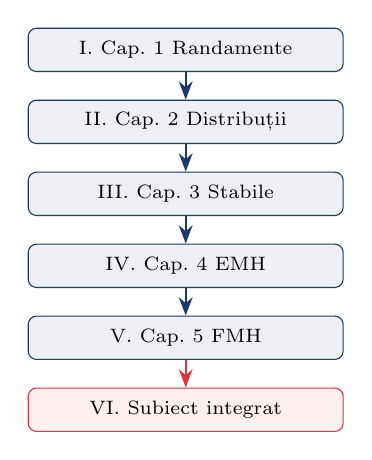
\begin{tikzpicture}[
    node distance=0.35cm,
    every node/.style={font=\scriptsize, align=center},
    phase/.style={draw=MainBlue, fill=MainBlue!8, rounded corners=3pt,
                  minimum width=4cm, minimum height=0.55cm}
]
\node[phase] (p1) {I. Cap.~1 Randamente};
\node[phase, below=of p1] (p2) {II. Cap.~2 Distribuții};
\node[phase, below=of p2] (p3) {III. Cap.~3 Stabile};
\node[phase, below=of p3] (p4) {IV. Cap.~4 EMH};
\node[phase, below=of p4] (p5) {V. Cap.~5 FMH};
\node[phase, below=of p5, fill=Crimson!8, draw=Crimson] (p6) {VI. Subiect integrat};
\draw[-{Stealth}, MainBlue, thick] (p1) -- (p2);
\draw[-{Stealth}, MainBlue, thick] (p2) -- (p3);
\draw[-{Stealth}, MainBlue, thick] (p3) -- (p4);
\draw[-{Stealth}, MainBlue, thick] (p4) -- (p5);
\draw[-{Stealth}, Crimson, thick] (p5) -- (p6);
\end{tikzpicture}
\end{center}
\end{column}
\end{columns}
    \end{cminipage}
\end{frame}

\begin{frame}[shrink=25]{Sinteza materiei --- ce acoperim}
\begin{cminipage}{0.95\textwidth}
\begin{columns}[T]
\begin{column}{0.52\textwidth}
\begin{block}{Capitole acoperite}
\small
\begin{itemize}\setlength{\itemsep}{0pt}
    \item \textbf{Cap.~1 --- Randamente și indicatori}
    \begin{itemize}\setlength{\itemsep}{0pt}
        \item Log-randamente, Sharpe, MDD, scalare $\sqrt T$
    \end{itemize}
    \item \textbf{Cap.~2 --- Distribuții clasice}
    \begin{itemize}\setlength{\itemsep}{0pt}
        \item Normal, Student-$t$, Pareto, VaR/ES, JB, AIC/BIC
    \end{itemize}
    \item \textbf{Cap.~3 --- Distribuții stabile}
    \begin{itemize}\setlength{\itemsep}{0pt}
        \item Parametri $(\alpha, \beta, \gamma, \delta)$, GCLT, McCulloch
    \end{itemize}
    \item \textbf{Cap.~4 --- Ipoteza Pieței Eficiente}
    \begin{itemize}\setlength{\itemsep}{0pt}
        \item Ljung--Box, runs, VR, event study, anomalii, AMH
    \end{itemize}
    \item \textbf{Cap.~5 --- Ipoteza Pieței Fractale (FMH)}
    \begin{itemize}\setlength{\itemsep}{0pt}
        \item Hurst, R/S, DFA, $D=2-H$, $T^H$, fBm
    \end{itemize}
\end{itemize}
\end{block}
\end{column}
\begin{column}{0.46\textwidth}
\begin{alertblock}{Valori critice utile}
\small
\begin{itemize}\setlength{\itemsep}{0pt}
    \item Cuantile normale
    \begin{itemize}\setlength{\itemsep}{0pt}
        \item $z_{0{,}05} = 1{,}645$
        \item $z_{0{,}025} = 1{,}96$
        \item $z_{0{,}01} = 2{,}326$
    \end{itemize}
    \item Cuantile $\chi^2$
    \begin{itemize}\setlength{\itemsep}{0pt}
        \item $\chi^2_2(0{,}05) = 5{,}99$
        \item $\chi^2_5(0{,}05) = 11{,}07$
        \item $\chi^2_{10}(0{,}05) = 18{,}31$
    \end{itemize}
\end{itemize}
\end{alertblock}
\end{column}
\end{columns}
\end{cminipage}
\end{frame}

%=============================================================================
% PARTEA I: CAP.1 --- RANDAMENTE
%=============================================================================
\section{Partea I: Cap.~1 --- Randamente și indicatori}

\begin{frame}[shrink=25]{Exercițiul 1: Log-randamente, Sharpe, drawdown}
\begin{cminipage}{0.95\textwidth}
\begin{columns}[T]
\begin{column}{0.55\textwidth}
\begin{block}{Enunț}
\begin{itemize}\setlength{\itemsep}{0pt}
    \item Se dau prețurile zilnice de închidere pentru o acțiune:
    \begin{itemize}\setlength{\itemsep}{0pt}
        \item $P_0 = 100$, $P_1 = 104$, $P_2 = 98$
        \item $P_3 = 106$, $P_4 = 92$, $P_5 = 95$
    \end{itemize}
    \item Date suplimentare:
    \begin{itemize}\setlength{\itemsep}{0pt}
        \item $R_f = 3\%$/an, 252 zile/an
    \end{itemize}
\end{itemize}
\end{block}
\end{column}
\begin{column}{0.42\textwidth}
\centering
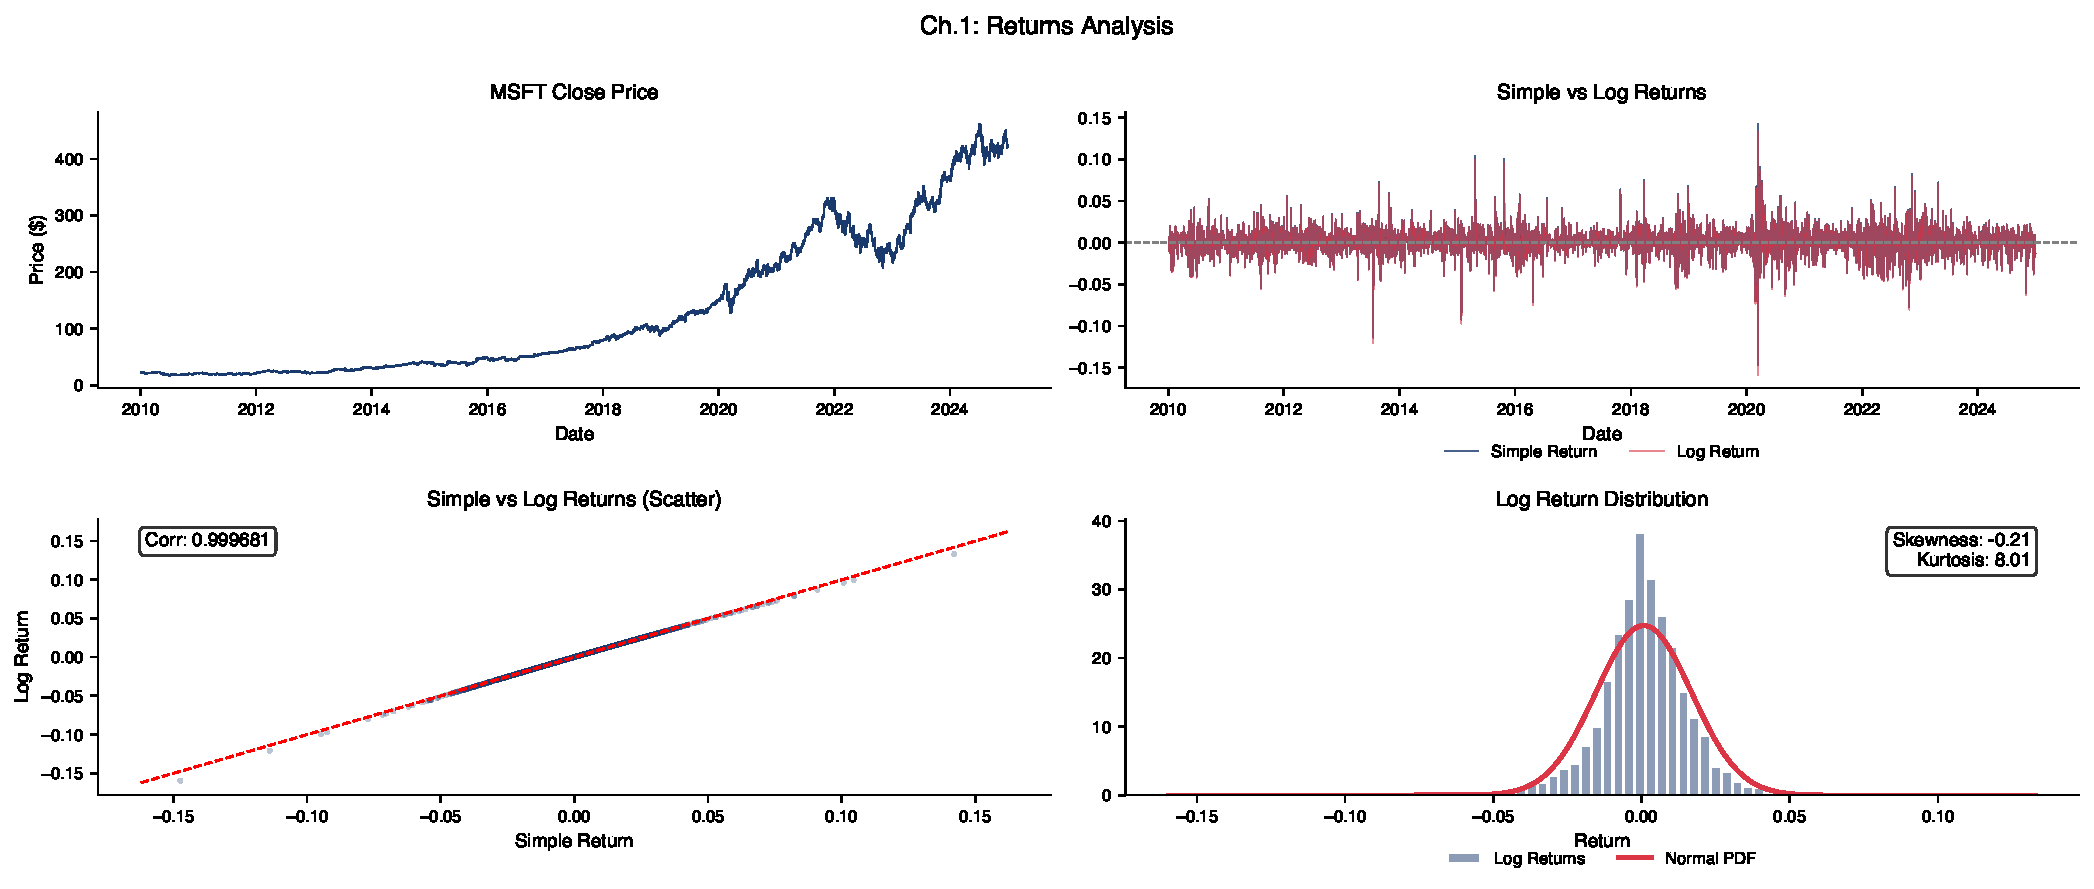
\includegraphics[width=\linewidth]{ch1_returns.pdf}\\[0.2em]
{\scriptsize \textit{Ilustrativ:} preț, randamente simple vs.\ log, distribuție pe un eșantion real}
\end{column}
\end{columns}
\vspace{0.05cm}
\quantlet{SFM\_ch1}{https://github.com/QuantLet/Stat_fin_markets/tree/master/Quantlets/SFM_ch1}
\begin{itemize}\setlength{\itemsep}{0pt}
    \item \textbf{Cerințe:}
    \begin{itemize}\setlength{\itemsep}{0pt}
        \item Calculați log-randamentele zilnice $r_t = \ln(P_t/P_{t-1})$ pentru $t = 1, \ldots, 5$ și interpretați semnul fiecăruia
        \item Calculați media eșantion $\bar{r}$, volatilitatea zilnică $\hat{\sigma}_{\text{zi}}$ și apoi anualizați volatilitatea folosind regula $\sqrt{T}$ cu $T = 252$ zile de tranzacționare
        \item Calculați indicatorul Sharpe anualizat folosind randamentul mediu anualizat, volatilitatea anualizată și rata fără risc $R_f = 3\%$
        \item Calculați Maximum Drawdown (MDD) al seriei de prețuri, identificând explicit running maximum la fiecare moment și cea mai mare pierdere procentuală relativă
        \item Interpretați economic rezultatele combinate: este activul atractiv din perspectiva raportului risc-randament și a pierderii maxime observate? Ce concluzii se pot trage pe un eșantion atât de scurt?
    \end{itemize}
\end{itemize}
\end{cminipage}
\end{frame}

\begin{frame}[shrink=25]{Exercițiul 1: Rezolvare}
\begin{cminipage}{0.95\textwidth}
\begin{exampleblock}{Rezolvare}
\small
\begin{itemize}\setlength{\itemsep}{0pt}
    \item \textbf{1. Log-randamente} \quad $r_t = \ln(P_t/P_{t-1})$
    \begin{itemize}\setlength{\itemsep}{0pt}
        \item $r_1 = 0{,}0392$,\ $r_2 = -0{,}0594$,\ $r_3 = 0{,}0784$,\ $r_4 = -0{,}1417$,\ $r_5 = 0{,}0321$
        \item \textit{Interpretare:} ziua 4 ($-14{,}2\%$) este un drop sever; semnele alternează --- volatilitate ridicată, fără tendință clară
    \end{itemize}
    \item \textbf{2. Statistici și anualizare} \quad $\bar r = \frac{1}{n}\sum r_t$;\ $\hat\sigma_{\text{an}} = \hat\sigma_{\text{zi}}\sqrt{252}$
    \begin{itemize}\setlength{\itemsep}{0pt}
        \item $\bar{r} = -0{,}0103$;\ $\hat{\sigma}_{\text{zi}} = 0{,}0853$;\ $\hat{\sigma}_{\text{an}} \approx 1{,}354$ ($135\%$)
        \item \textit{Interpretare:} volatilitatea anualizată $> 100\%$ este enormă; tipic pentru cripto ultra-speculativ, nu pentru acțiuni stabile
    \end{itemize}
    \item \textbf{3. Sharpe} \quad $\text{SR} = (\hat\mu_{\text{an}} - R_f) / \hat\sigma_{\text{an}}$
    \begin{itemize}\setlength{\itemsep}{0pt}
        \item $\hat{\mu}_{\text{an}} = -2{,}60$;\ $\text{SR} = (-2{,}60 - 0{,}03)/1{,}354 \approx \mathbf{-1{,}94}$
        \item \textit{Interpretare:} Sharpe puternic negativ $\Rightarrow$ pe această fereastră activul a generat $1{,}94\sigma$ \emph{sub} rata fără risc; dezastruos
    \end{itemize}
    \item \textbf{4. MDD} \quad $\text{MDD} = \min_t \frac{P_t - \max_{s \le t} P_s}{\max_{s \le t} P_s}$
    \begin{itemize}\setlength{\itemsep}{0pt}
        \item Running max: $100, 104, 104, 106, 106, 106$ $\Rightarrow$ MDD $= (92 - 106)/106 \approx \mathbf{-13{,}21\%}$
        \item \textit{Interpretare:} dintr-un peak de $106$, prețul a căzut la $92$ --- pierdere maximă de $13{,}2\%$ pe care un investitor ar fi simțit-o ca \emph{realizată} dacă ar fi cumpărat la peak
    \end{itemize}
    \item \textbf{5. Concluzie integrată:}
    \begin{itemize}\setlength{\itemsep}{0pt}
        \item Sharpe negativ + MDD mare $\Rightarrow$ activ neatractiv pe fereastra dată
        \item \textbf{Avertisment metodologic:} $n = 5$ este complet insuficient; anualizarea cu $\sqrt{252}$ extrapolează zgomotul a 5 zile la 1 an. În practică se cere $n \ge 250$ pentru estimări robuste
    \end{itemize}
\end{itemize}
\end{exampleblock}
\end{cminipage}
\end{frame}

\begin{frame}[shrink=25]{Exercițiul 2: Variance Drag și regula $\sqrt{T}$}
\begin{cminipage}{0.95\textwidth}
\begin{block}{Enunț}
\begin{itemize}\setlength{\itemsep}{0pt}
    \item Un fond de investiții are următorii parametri:
    \begin{itemize}\setlength{\itemsep}{0pt}
        \item Randament aritmetic așteptat $\E[R] = 10\%$ anual
        \item Volatilitate anuală $\sigma = 25\%$
    \end{itemize}
    \item \textbf{Cerințe:}
    \begin{itemize}\setlength{\itemsep}{0pt}
        \item Aproximați randamentul geometric așteptat folosind formula variance drag $\E[r] \approx \E[R] - \sigma^2/2$ și calculați cât reprezintă pierderea din varianță
        \item Calculați averea finală după 20 ani pentru o investiție inițială $W_0 = 1$ folosind compunerea continuă $W_T = W_0 e^{T \cdot \E[r]}$ și comparați cu rezultatul ``naiv'' $(1+\E[R])^T$
        \item Presupunând o volatilitate zilnică $\sigma_{\text{zi}} = 1{,}5\%$ sub ipoteza i.i.d., calculați volatilitatea săptămânală (5 zile) și anualizată (252 zile) folosind regula $\sqrt{T}$
        \item Discutați cum se modifică volatilitatea anualizată dacă randamentele prezintă autocorelație pozitivă $\hat\rho_1 = 0{,}10 > 0$: crește sau scade față de estimarea i.i.d.? Justificați prin formula extinsă a varianței sumei
    \end{itemize}
\end{itemize}
\end{block}
\end{cminipage}
\end{frame}

\begin{frame}[shrink=25]{Exercițiul 2: Rezolvare}
\begin{cminipage}{0.95\textwidth}
\begin{exampleblock}{Rezolvare}
\begin{itemize}\setlength{\itemsep}{0pt}
    \item \textbf{1. Variance drag} \quad $\E[r] \approx \E[R] - \sigma^2/2$
    \begin{itemize}\setlength{\itemsep}{0pt}
        \item $\E[r] \approx 0{,}10 - 0{,}03125 = \mathbf{0{,}0688}$;\ pierdere $3{,}12\%$/an
        \item \textit{Interpretare:} compunerea geometrică nu e simetrică; o pierdere de $50\%$ urmată de un câștig de $50\%$ ajunge la $75\%$, nu $100\%$. Cu cât $\sigma$ e mai mare, cu atât drag-ul e mai sever (relație pătratică)
    \end{itemize}
    \item \textbf{2. Averea finală} \quad $W_T = W_0 e^{T \cdot \E[r]}$
    \begin{itemize}\setlength{\itemsep}{0pt}
        \item $W_{20} = e^{1{,}375} \approx \mathbf{3{,}95}$ vs.\ naiv $(1{,}10)^{20} = 6{,}73$
        \item \textit{Interpretare:} diferență de $\mathbf{2{,}78\times}$ pe 20 ani --- ignorarea variance drag-ului supraestimează grav averea așteptată. Niciodată nu folosim aritmeticul pentru CAGR
    \end{itemize}
    \item \textbf{3. Anualizare sub i.i.d.} \quad $\sigma_T = \sigma_1 \sqrt{T}$
    \begin{itemize}\setlength{\itemsep}{0pt}
        \item $\sigma_{\text{săpt}} \approx 3{,}35\%$;\ $\sigma_{\text{an}} \approx 23{,}8\%$
        \item \textit{Interpretare:} regula $\sqrt T$ presupune \emph{independență}; valabilă strict sub i.i.d. Empiric, randamentele financiare au $H \in [0{,}5, 0{,}65]$ pe orizont lung $\Rightarrow$ regula e doar o aproximație
    \end{itemize}
    \item \textbf{4. Corecție cu autocorelație} \quad $\sigma^2_T = T\sigma^2_1\left(1 + 2\sum_{k}\frac{T-k}{T}\rho_k\right)$
    \begin{itemize}\setlength{\itemsep}{0pt}
        \item $\rho_1 > 0 \Rightarrow \sigma_{\text{an}}$ reală \textbf{mai mare} decât cea i.i.d.
        \item \textit{Interpretare:} momentum (persistență) amplifică riscul pe orizont lung; $\sqrt T$ subestimează. Pentru piețe persistente alternativa este $\sigma_T \sim T^H$ (FMH, Cap.~5). Pe S\&P 500 eroarea e mică ($H \approx 0{,}53$); pe BVB devine relevantă ($H \approx 0{,}6$)
    \end{itemize}
\end{itemize}
\end{exampleblock}

\begin{alertblock}{Greșeală frecventă}
\begin{itemize}\setlength{\itemsep}{0pt}
    \item Confuzie aritmetic vs geometric
    \begin{itemize}\setlength{\itemsep}{0pt}
        \item Pe orizont lung se folosește \textbf{geometric}, nu aritmetic
    \end{itemize}
\end{itemize}
\end{alertblock}
\end{cminipage}
\end{frame}

\begin{frame}[shrink=25]{Exercițiul 3: Asimetrie, kurtosis și regimuri de risc}
\begin{cminipage}{0.95\textwidth}
\begin{block}{Enunț}
\begin{itemize}\setlength{\itemsep}{0pt}
    \item Se compară două active ($R_f = 2\%$):
    \begin{itemize}\setlength{\itemsep}{0pt}
        \item Activ A (blue-chip): $\hat\mu_{\text{an}} = 8\%$, $\hat\sigma_{\text{an}} = 18\%$, $S = -0{,}2$, $\kappa = 1{,}5$
        \item Activ B (crypto): $\hat\mu_{\text{an}} = 25\%$, $\hat\sigma_{\text{an}} = 80\%$, $S = -1{,}8$, $\kappa = 12$
    \end{itemize}
    \item \textbf{Cerințe:}
    \begin{itemize}\setlength{\itemsep}{0pt}
        \item Calculați explicit indicatorul Sharpe pentru ambele active folosind $\text{SR} = (\hat\mu - R_f)/\hat\sigma$ și comparați
        \item Identificați care dintre cele două active prezintă un risc mai mare de coadă stângă (pierderi extreme), argumentând pe baza combinației dintre asimetria $S$ și kurtosis $\kappa$
        \item Discutați dacă estimarea VaR sub ipoteza de normalitate este fiabilă pentru activul B; justificați cu un calcul al probabilității unui eveniment $5\sigma$ sub normală vs. frecvența empirică așteptată
        \item Recomandați explicit o distribuție alternativă pentru activul B (Student-$t$, stabilă, Pareto) și justificați alegerea prin compatibilitatea cu $S$ și $\kappa$ observate
    \end{itemize}
\end{itemize}
\end{block}
\end{cminipage}
\end{frame}

\begin{frame}[shrink=25]{Exercițiul 3: Rezolvare}
\begin{cminipage}{0.95\textwidth}
\begin{exampleblock}{Rezolvare}
\begin{itemize}\setlength{\itemsep}{0pt}
    \item \textbf{1. Sharpe} \quad $\text{SR} = (\hat\mu - R_f)/\hat\sigma$
    \begin{itemize}\setlength{\itemsep}{0pt}
        \item Activ A: $\mathbf{0{,}33}$;\ Activ B: $\mathbf{0{,}29}$
        \item \textit{Interpretare:} A iese mai bine pe Sharpe \emph{deși} are randament mai mic --- normalizarea cu $\sigma$ penalizează B sever. Capcană: Sharpe presupune Gaussian, ignoră $S, K$, MDD
    \end{itemize}
    \item \textbf{2. Risc de coadă stângă:}
    \begin{itemize}\setlength{\itemsep}{0pt}
        \item B: $S = -1{,}8$ (asimetrie puternic negativă), $\kappa = 12$ (cozi foarte groase)
        \item \textit{Interpretare:} combinația $S \ll 0$ și $\kappa \gg 0$ semnalizează crash-uri asimetrice (downside risk) --- Sharpe nu detectează acest risc. Investitorul real ar prefera A datorită profilului mai puțin coadă-grea
    \end{itemize}
    \item \textbf{3. VaR normală pentru B:}
    \begin{itemize}\setlength{\itemsep}{0pt}
        \item Eveniment $5\sigma$ sub normală: $P \approx 3 \cdot 10^{-7}$ ($\sim 1$/$10.000$ ani)
        \item \textit{Interpretare:} empiric, șocuri $5\sigma$ apar la $\sim 1$/$5$ ani pe BTC $\Rightarrow$ subestimare cu factor $\sim 2.000$. VaR Normal pentru B este \textbf{periculos}
    \end{itemize}
    \item \textbf{4. Distribuții alternative pentru B:}
    \begin{itemize}\setlength{\itemsep}{0pt}
        \item Student-$t$ cu $\nu \in [4, 6]$ (captează kurtosis $K = 12$ via $\nu = 4 + 6/9 \approx 4{,}7$)
        \item Stabilă cu $\alpha < 2$, $\beta < 0$ (cozi $+$ asimetrie simultan)
        \item Pareto/GPD pe coadă stângă (POT --- Peak-Over-Threshold)
        \item \textit{Interpretare:} alegerea depinde de scop: Student-$t$ pentru VaR uzual, GPD pentru stress-test, Stable pentru consistență teoretică (GCLT)
    \end{itemize}
\end{itemize}
\end{exampleblock}
\end{cminipage}
\end{frame}

%=============================================================================
% PARTEA II: CAP.2 --- DISTRIBUTII CLASICE
%=============================================================================
\section{Partea II: Cap.~2 --- Distribuții clasice}

\begin{frame}[shrink=25]{Exercițiul 4: Normalitate --- testul Jarque--Bera}
\begin{cminipage}{0.95\textwidth}
\begin{block}{Enunț}
\begin{itemize}\setlength{\itemsep}{0pt}
    \item Eșantion de $n = 500$ randamente zilnice S\&P~500:
    \begin{itemize}\setlength{\itemsep}{0pt}
        \item $\bar{r} = 0{,}0004$; $\hat\sigma = 0{,}012$
        \item Asimetrie $S = -0{,}42$; kurtosis $K = 6{,}8$
    \end{itemize}
    \item \textbf{Cerințe:}
    \begin{itemize}\setlength{\itemsep}{0pt}
        \item Calculați explicit statistica Jarque--Bera folosind $JB = \frac{n}{6}\left(S^2 + \frac{(K-3)^2}{4}\right)$, detaliind separat contribuțiile asimetriei și kurtosis
        \item Testați ipoteza nulă $H_0$ de normalitate la pragul de semnificație $\alpha = 5\%$, folosind valoarea critică $\chi^2_2(0{,}05) = 5{,}99$ și formulați decizia
        \item Enumerați cel puțin 3 ``fapte stilizate'' ale randamentelor financiare (Cont, 2001) care contrazic ipoteza de normalitate și explicați succint fiecare
        \item Calibrați parametrul $\nu$ al unei distribuții Student-$t$ care ar produce același kurtosis $K = 6{,}8$ ca cel observat, folosind formula $\kappa = K - 3 = 6/(\nu - 4)$
    \end{itemize}
\end{itemize}
\end{block}
\end{cminipage}
\end{frame}

\begin{frame}[shrink=25]{Exercițiul 4: Rezolvare}
\begin{cminipage}{0.95\textwidth}
\begin{exampleblock}{Rezolvare}
\begin{itemize}\setlength{\itemsep}{0pt}
    \item \textbf{1. Calcul JB} \quad $JB = \dfrac{n}{6}\left(S^2 + \dfrac{(K-3)^2}{4}\right) \xrightarrow{H_0} \chi^2_2$
    \begin{itemize}\setlength{\itemsep}{0pt}
        \item $S^2 = 0{,}1764$;\ $(K-3)^2/4 = 3{,}61$;\ $JB \approx \mathbf{315{,}5}$
        \item \textit{Interpretare:} contribuția kurtozei ($3{,}61$) domină asimetria ($0{,}18$) cu $20\times$ --- cozile groase sunt sursa principală de neGaussianitate, mai mult decât asimetria
    \end{itemize}
    \item \textbf{2. Decizia} \quad respingem $H_0$ dacă $JB > \chi^2_2(0{,}05) = 5{,}99$
    \begin{itemize}\setlength{\itemsep}{0pt}
        \item $JB = 315{,}5 \gg 5{,}99$ $\Rightarrow$ respingem $H_0$ covârșitor; $p \approx 10^{-69}$
        \item \textit{Interpretare:} $JB = 315$ este astronomic --- normalitatea e respinsă cu o certitudine practic absolută. Empiric, JB respinge normalitatea pe \emph{orice} serie financiară cu $n > 500$
    \end{itemize}
    \item \textbf{3. Fapte stilizate contra normalității} (Cont, 2001):
    \begin{itemize}\setlength{\itemsep}{0pt}
        \item Cozi groase ($K > 3$) și asimetrie negativă ($S < 0$)
        \item Clustering de volatilitate, efect de leverage
        \item Memorie lungă pe pătrate (efect GARCH)
        \item \textit{Interpretare:} normalitatea e o aproximare pedagogică convenabilă, dar pentru risc management este periculoasă (subestimează crash-uri)
    \end{itemize}
    \item \textbf{4. Calibrare Student-$t$} \quad $\kappa = K - 3 = 6/(\nu - 4),\ \nu > 4$
    \begin{itemize}\setlength{\itemsep}{0pt}
        \item $\kappa = 3{,}8 \Rightarrow \nu = 4 + 6/3{,}8 \approx \mathbf{5{,}58}$
        \item \textit{Interpretare:} $\nu \approx 5$--$6$ este standard pentru indici acțiuni; pentru cripto $\nu \approx 3$--$4$. Nota: $\nu = 5{,}58$ are momentul 4 finit dar al 6-lea infinit
    \end{itemize}
\end{itemize}
\end{exampleblock}
\end{cminipage}
\end{frame}

\begin{frame}[shrink=25]{Anexă vizuală Ex.~4: QQ-plot --- normalitate vs.\ alternative}
\begin{cminipage}{0.95\textwidth}
\begin{columns}[T]
\begin{column}{0.62\textwidth}
\centering
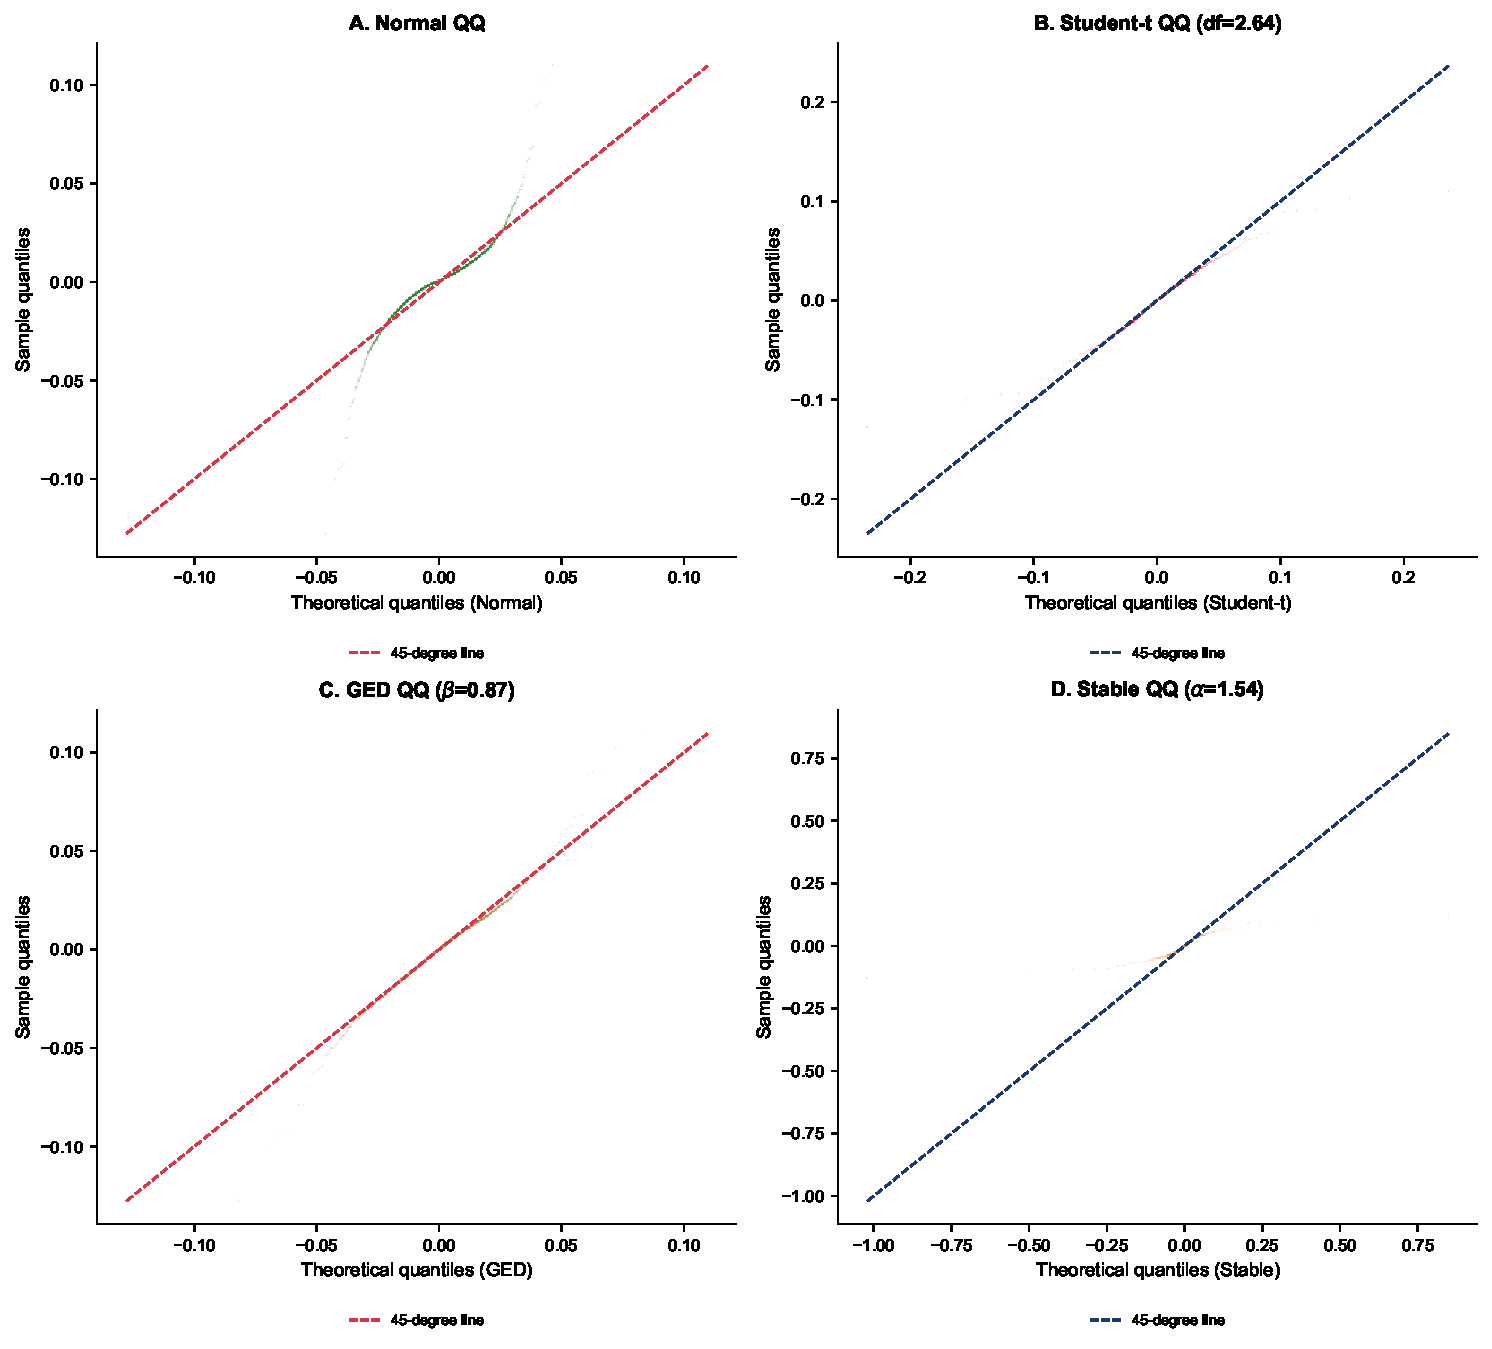
\includegraphics[width=0.82\linewidth]{ch2_dist_comparison_qq.pdf}\\[0.2em]
\quantlet{SFM\_ch2}{https://github.com/QuantLet/Stat_fin_markets/tree/master/Quantlets/SFM_ch2}
\end{column}
\begin{column}{0.36\textwidth}
\begin{block}{Citirea graficului}
\begin{itemize}\setlength{\itemsep}{0pt}
    \item \textbf{A. Normal QQ}: capete \emph{deviate} de la linia 45° $\Rightarrow$ cozi mai groase decât Normala
    \item \textbf{B. Student-$t$ QQ ($\nu = 2{,}64$)}: aliniere bună $\Rightarrow$ Student-$t$ captează cozile
    \item \textbf{C. GED QQ ($\beta = 0{,}87$)}: aliniere bună
    \item \textbf{D. Stable QQ ($\alpha = 1{,}54$)}: aliniere foarte bună --- cea mai apropiată de date
\end{itemize}
\end{block}
\begin{exampleblock}{De ce conteză}
Diagnosticul vizual completează JB: deviațiile de la 45° \emph{în care zonă} (centru / cozi) ne spun ce model alternativ să alegem.
\end{exampleblock}
\end{column}
\end{columns}
\end{cminipage}
\end{frame}

\begin{frame}[shrink=25]{Exercițiul 5: VaR și ES --- Normal vs Student-$t$ vs Pareto}
\begin{cminipage}{0.95\textwidth}
\begin{block}{Enunț}
\begin{itemize}\setlength{\itemsep}{0pt}
    \item Portofoliu de \$10M cu $\hat\sigma_{\text{zi}} = 1{,}5\%$, $\mu \approx 0$:
    \begin{itemize}\setlength{\itemsep}{0pt}
        \item Estimator Hill pe coada stângă: $\hat\alpha = 3{,}5$
    \end{itemize}
    \item \textbf{Cerințe:} calculați VaR 1\% zilnic sub:
    \begin{itemize}\setlength{\itemsep}{0pt}
        \item Normal ($z_{0{,}01} = 2{,}326$)
        \item Student-$t$ cu $\nu = 5$ ($|t_5^{-1}(0{,}01)| = 3{,}365$); $s = \sigma\sqrt{(\nu-2)/\nu}$
        \item Pareto: $\text{VaR} = x_m \cdot (1/\alpha)^{-1/\alpha}$, $x_m = 1\%$, $\alpha = 3{,}5$
    \end{itemize}
    \item \textbf{Analize:}
    \begin{itemize}\setlength{\itemsep}{0pt}
        \item Care model avertizează cel mai sever și de ce?
        \item Calculați $\text{ES}/\text{VaR}$ Pareto: $\alpha/(\alpha-1)$
    \end{itemize}
\end{itemize}
\end{block}
\end{cminipage}
\end{frame}

\begin{frame}[shrink=25]{Exercițiul 5: Rezolvare}
\begin{cminipage}{0.95\textwidth}
\begin{exampleblock}{Rezolvare}
\begin{itemize}\setlength{\itemsep}{0pt}
    \item \textbf{1. VaR Normal} \quad $\text{VaR}_\alpha = -(\mu + z_\alpha \sigma) \cdot W \approx z_\alpha \sigma W$
    \begin{itemize}\setlength{\itemsep}{0pt}
        \item $\text{VaR} = 2{,}326 \cdot 0{,}015 \cdot 10\text{M} = \mathbf{\$348.900}$
    \end{itemize}
    \item \textbf{2. VaR Student-$t$ ($\nu=5$)} \quad $\text{VaR} = |t_\nu^{-1}(\alpha)| \cdot s \cdot W$;\ $s = \sigma\sqrt{(\nu-2)/\nu}$
    \begin{itemize}\setlength{\itemsep}{0pt}
        \item $s = 0{,}015 \cdot \sqrt{3/5} = 0{,}01162$
        \item $\text{VaR} = 3{,}365 \cdot 0{,}01162 \cdot 10\text{M} = \mathbf{\$390.800}$
    \end{itemize}
    \item \textbf{3. VaR Pareto ($\alpha = 3{,}5$)} \quad $\text{VaR} = x_m \cdot \alpha^{1/\alpha}$ (pe randament; aici $x_m \cdot p^{-1/\alpha}$ pentru cuantilă)
    \begin{itemize}\setlength{\itemsep}{0pt}
        \item $\text{VaR} = 0{,}01 \cdot (0{,}01)^{-1/3{,}5} = 0{,}01 \cdot 3{,}727 \approx 0{,}0373$
        \item $\text{VaR} \approx \mathbf{\$372.700}$
    \end{itemize}
    \item \textbf{4. Comparație:}
    \begin{itemize}\setlength{\itemsep}{0pt}
        \item Student-$t$ și Pareto depășesc Normal cu $\sim 10$--$15\%$
        \item \textit{Interpretare:} pentru o bancă, diferența $\$348k$ vs $\$390k$ pe \$10M se traduce direct în capital regulamentar (Basel III/FRTB). $12\%$ subestimare $=$ provizioane insuficiente
        \item Pareto sensibilă la $\alpha$: pentru $\alpha \to 2$, VaR Pareto explodează (varianța devine infinită la limită)
    \end{itemize}
    \item \textbf{5. Raport ES/VaR} \quad Pareto: $\text{ES}/\text{VaR} = \alpha/(\alpha-1)$ pentru $\alpha > 1$
    \begin{itemize}\setlength{\itemsep}{0pt}
        \item Pareto: $\mathbf{1{,}40}$;\ Student-$t(\nu=5)$: $\approx 1{,}28$;\ Normal: $\approx 1{,}15$
        \item \textit{Interpretare:} cu cât distribuția e mai coadă-grea, cu atât ES (Expected Shortfall, ce \emph{înseamnă} pierderea când VaR e depășit) este mai mare relativ la VaR. Basel III a adoptat ES tocmai pentru a captura coada
    \end{itemize}
\end{itemize}
\end{exampleblock}
\end{cminipage}
\end{frame}

\begin{frame}[shrink=25]{Exercițiul 6: Selecție de model --- AIC și BIC}
\begin{cminipage}{0.95\textwidth}
\begin{block}{Enunț}
\begin{itemize}\setlength{\itemsep}{0pt}
    \item Pe un eșantion $n = 1.000$, MLE produce:
    \begin{itemize}\setlength{\itemsep}{0pt}
        \item Normal: $\ell = 3.150{,}2$, $k = 2$
        \item Student-$t$: $\ell = 3.188{,}7$, $k = 3$
        \item Stabilă: $\ell = 3.192{,}1$, $k = 4$
    \end{itemize}
    \item \textbf{Cerințe:}
    \begin{itemize}\setlength{\itemsep}{0pt}
        \item Calculați explicit criteriile AIC $= -2\ell + 2k$ și BIC $= -2\ell + k\ln n$ pentru fiecare dintre cele 3 modele, detaliind calculul pentru fiecare
        \item Stabiliți care dintre modele este preferat de criteriul AIC (cel cu AIC minim) și care este preferat de criteriul BIC, explicând semnificația diferenței
        \item Explicați de ce criteriul BIC penalizează mai sever complexitatea modelului decât AIC pentru eșantioane mari, pornind de la comparația termenilor de penalizare $2k$ vs $k \ln n$
    \end{itemize}
    \item \textbf{Formule și convenții:}
    \begin{itemize}\setlength{\itemsep}{0pt}
        \item Modelul cu AIC sau BIC \textit{minim} este preferat
        \item Regulă empirică: $\Delta\text{AIC} < 2$ $\Rightarrow$ modele echivalente; $\Delta > 10$ $\Rightarrow$ alegere clară
    \end{itemize}
\end{itemize}
\end{block}
\end{cminipage}
\end{frame}

\begin{frame}[shrink=25]{Exercițiul 6: Rezolvare}
\begin{cminipage}{0.95\textwidth}
\begin{exampleblock}{Rezolvare}
\small
\begin{itemize}\setlength{\itemsep}{0pt}
    \item \textbf{1. AIC} \quad $\text{AIC} = -2\ell + 2k$ \quad (preferăm minim)
    \begin{itemize}\setlength{\itemsep}{0pt}
        \item Normal: $-6.300{,}4 + 4 = \mathbf{-6.296{,}4}$
        \item Student-$t$: $-6.377{,}4 + 6 = \mathbf{-6.371{,}4}$
        \item Stabilă: $-6.384{,}2 + 8 = \mathbf{-6.376{,}2}$
    \end{itemize}
    \item \textbf{2. BIC} \quad $\text{BIC} = -2\ell + k\ln n$,\ $\ln 1000 = 6{,}908$
    \begin{itemize}\setlength{\itemsep}{0pt}
        \item Normal: $-6.300{,}4 + 13{,}82 = \mathbf{-6.286{,}6}$
        \item Student-$t$: $-6.377{,}4 + 20{,}72 = \mathbf{-6.356{,}7}$
        \item Stabilă: $-6.384{,}2 + 27{,}63 = \mathbf{-6.356{,}6}$
    \end{itemize}
    \item \textbf{3. Alegerea modelului:}
    \begin{itemize}\setlength{\itemsep}{0pt}
        \item AIC preferă Stabilă (cel mai mic)
        \item BIC: Student-$t$ și Stabilă aproape egale ($\Delta < 1$), Student-$t$ marginal mai bună
        \item \textit{Interpretare:} divergența AIC vs BIC pe \emph{același} eșantion semnalează că diferența între Student-$t$ și Stabilă este \emph{marginală} (sub $\Delta$BIC $= 2$ $\Rightarrow$ ``echivalent practic''). Decizia finală se face pe argumente teoretice: Stable e consistent cu GCLT, Student-$t$ e mai ușor de implementat
    \end{itemize}
    \item \textbf{4. Penalizare BIC vs AIC} \quad pentru $n = 1000$: $\ln n = 6{,}91 > 2$
    \begin{itemize}\setlength{\itemsep}{0pt}
        \item BIC penalizează fiecare parametru cu $\ln n$, AIC doar cu $2$
        \item \textit{Interpretare:} BIC e \emph{consistent} (alege modelul adevărat când $n \to \infty$, dacă acest model e în clasă); AIC tinde să suprasaturate. Regulă practică: pentru $n > 100$, BIC e preferat în model selection riguros
    \end{itemize}
\end{itemize}
\end{exampleblock}
\end{cminipage}
\end{frame}

%=============================================================================
% EXERCITII ALTERNATIVE CAP.2 (FARA VaR/ES)
%=============================================================================

\begin{frame}[shrink=25]{Exercițiul 6b: Probabilități de evenimente extreme}
\begin{cminipage}{0.95\textwidth}
\begin{block}{Enunț}
\begin{itemize}\setlength{\itemsep}{0pt}
    \item Un portofoliu are randament zilnic cu $\mu = 0$ și $\sigma_{\text{zi}} = 1\%$
    \begin{itemize}\setlength{\itemsep}{0pt}
        \item Model 1: $r_t/\sigma \sim \mathcal{N}(0, 1)$
        \item Model 2: $r_t/\sigma \sim t_5$ (Student-$t$ cu $\nu = 5$)
    \end{itemize}
    \item Cuantile de referință:
    \begin{itemize}\setlength{\itemsep}{0pt}
        \item $\Phi(-3) = 0{,}00135$; $\Phi(-4) = 3{,}17 \cdot 10^{-5}$
        \item $P(t_5 < -3) \approx 0{,}0150$; $P(t_5 < -4) \approx 0{,}0052$
    \end{itemize}
    \item \textbf{Cerințe:}
    \begin{itemize}\setlength{\itemsep}{0pt}
        \item Calculați $P(r_t < -3\%)$ sub fiecare model
        \item Câte zile extreme ($r < -3\%$) așteptați în $n = 1000$ zile?
        \item Calculați raportul probabilităților Student-$t$/Normal la $3\sigma$ și $4\sigma$
        \item Ce vă spune evoluția acestui raport despre comportamentul cozilor?
    \end{itemize}
\end{itemize}
\end{block}
\end{cminipage}
\end{frame}

\begin{frame}[shrink=25]{Exercițiul 6b: Rezolvare}
\begin{cminipage}{0.95\textwidth}
\begin{exampleblock}{Rezolvare}
\begin{itemize}\setlength{\itemsep}{0pt}
    \item \textbf{1. Probabilități la $3\sigma$:}
    \begin{itemize}\setlength{\itemsep}{0pt}
        \item Normal: $P(r < -3\%) = \Phi(-3) = 0{,}00135 = 0{,}135\%$
        \item Student-$t$: $P(r < -3\%) = P(t_5 < -3) \approx 0{,}0150 = 1{,}50\%$
    \end{itemize}
    \item \textbf{2. Zile extreme așteptate în 1000 zile:}
    \begin{itemize}\setlength{\itemsep}{0pt}
        \item Normal: $1000 \cdot 0{,}00135 \approx 1{,}35$ zile ($\sim 1$ zi în $740$)
        \item Student-$t$: $1000 \cdot 0{,}0150 = 15$ zile ($\sim 1$ zi în $67$)
    \end{itemize}
    \item \textbf{3. Rapoarte Student-$t$/Normal:}
    \begin{itemize}\setlength{\itemsep}{0pt}
        \item La $3\sigma$: $0{,}0150/0{,}00135 \approx \mathbf{11{,}1\times}$
        \item La $4\sigma$: $0{,}0052/(3{,}17 \cdot 10^{-5}) \approx \mathbf{164\times}$
    \end{itemize}
    \item \textbf{4. Interpretare:}
    \begin{itemize}\setlength{\itemsep}{0pt}
        \item Raportul \textbf{crește exploziv} cu nivelul de extremitate
        \item Cauza: cozile Student-$t$ scad polinomial $|x|^{-(\nu+1)}$
        \item Cozile Normalei scad super-exponențial $e^{-x^2/2}$
        \item Pentru evenimente rare, Student-$t$ alocă fundamental mai multă probabilitate
    \end{itemize}
\end{itemize}
\end{exampleblock}
\end{cminipage}
\end{frame}

\begin{frame}[shrink=25]{Exercițiul 6c: Calibrarea Student-$t$ din kurtosis}
\begin{cminipage}{0.95\textwidth}
\begin{block}{Enunț}
\begin{itemize}\setlength{\itemsep}{0pt}
    \item Pe un activ se estimează empiric:
    \begin{itemize}\setlength{\itemsep}{0pt}
        \item Kurtosis $K = 7{,}5$ (exces $\kappa = K - 3 = 4{,}5$)
        \item Volatilitate zilnică $\sigma_{\text{obs}} = 1{,}2\%$
    \end{itemize}
    \item Formule utile pentru Student-$t$ cu parametrul de scală $s$:
    \begin{itemize}\setlength{\itemsep}{0pt}
        \item $\kappa_{\text{Student-}t} = 6/(\nu - 4)$, $\nu > 4$
        \item $\Var(r) = s^2 \cdot \nu/(\nu - 2)$, $\nu > 2$
    \end{itemize}
    \item \textbf{Cerințe:}
    \begin{itemize}\setlength{\itemsep}{0pt}
        \item Calculați $\nu$ implicit pentru Student-$t$
        \item Care sunt momentele finite ale lui Student-$t$ cu acest $\nu$?
        \item Calculați scala $s$ astfel încât $\Var(r) = \sigma_{\text{obs}}^2$
        \item Comparați rata de scădere a cozilor: Student-$t$ vs Normal
    \end{itemize}
\end{itemize}
\end{block}
\end{cminipage}
\end{frame}

\begin{frame}[shrink=25]{Exercițiul 6c: Rezolvare}
\begin{cminipage}{0.95\textwidth}
\begin{exampleblock}{Rezolvare}
\begin{itemize}\setlength{\itemsep}{0pt}
    \item \textbf{1. Grade de libertate implicite:}
    \begin{itemize}\setlength{\itemsep}{0pt}
        \item $\kappa = 4{,}5 = 6/(\nu - 4) \Rightarrow \nu - 4 = 6/4{,}5 = 1{,}33$
        \item $\nu \approx \mathbf{5{,}33}$
    \end{itemize}
    \item \textbf{2. Momente finite:}
    \begin{itemize}\setlength{\itemsep}{0pt}
        \item Finite doar pentru ordin $p < \nu = 5{,}33$
        \item Medie, varianță, asimetrie, kurtosis --- toate finite ($1, 2, 3, 4 < 5{,}33$)
        \item Momente $\ge 6$ --- infinite
    \end{itemize}
    \item \textbf{3. Scala $s$:}
    \begin{itemize}\setlength{\itemsep}{0pt}
        \item $s = \sigma_{\text{obs}} \cdot \sqrt{(\nu - 2)/\nu} = 0{,}012 \cdot \sqrt{3{,}33/5{,}33}$
        \item $s = 0{,}012 \cdot 0{,}790 \approx \mathbf{0{,}00948}$ ($\approx 0{,}95\%$)
    \end{itemize}
    \item \textbf{4. Rata de scădere a cozilor:}
    \begin{itemize}\setlength{\itemsep}{0pt}
        \item Student-$t(\nu = 5{,}33)$: $f(x) \propto |x|^{-(\nu+1)} = |x|^{-6{,}33}$ (polinomial)
        \item Normal: $f(x) \propto e^{-x^2/2}$ (super-exponențial)
        \item Pentru $|x|$ mare, cozile Student-$t$ sunt mult mai groase $\Rightarrow$ captează evenimentele extreme
    \end{itemize}
\end{itemize}
\end{exampleblock}
\end{cminipage}
\end{frame}

%=============================================================================
% PARTEA III: CAP.3 --- DISTRIBUTII STABILE
%=============================================================================
\section{Partea III: Cap.~3 --- Distribuții stabile}

\begin{frame}[shrink=25]{Exercițiul 7: Parametrii distribuției stabile}
\begin{cminipage}{0.95\textwidth}
\begin{block}{Enunț}
\begin{itemize}\setlength{\itemsep}{0pt}
    \item Pe randamente zilnice Ethereum, MLE produce:
    \begin{itemize}\setlength{\itemsep}{0pt}
        \item $S(\alpha, \beta, \gamma, \delta) = S(1{,}58;\; -0{,}22;\; 0{,}018;\; -0{,}001)$
    \end{itemize}
    \item \textbf{Cerințe:}
    \begin{itemize}\setlength{\itemsep}{0pt}
        \item Interpretați economic fiecare parametru
        \item Sunt varianța și kurtosis finite? Care este cel mai mare moment finit?
        \item Cum se compară cozile cu Normala ($\alpha = 2$) și Cauchy ($\alpha = 1$)?
        \item Ce implică $\beta < 0$ pentru riscul asimetric?
        \item Pe ce interval variază $\alpha, \beta, \gamma, \delta$?
    \end{itemize}
\end{itemize}
\end{block}
\end{cminipage}
\end{frame}

\begin{frame}[shrink=25]{Exercițiul 7: Rezolvare}
\begin{cminipage}{0.95\textwidth}
\begin{exampleblock}{Rezolvare}
\begin{itemize}\setlength{\itemsep}{0pt}
    \item \textbf{1. Interpretarea parametrilor} \quad $S(\alpha, \beta, \gamma, \delta)$
    \begin{itemize}\setlength{\itemsep}{0pt}
        \item $\alpha = 1{,}58$: cozi groase (între Cauchy $\alpha=1$ și Normal $\alpha=2$)
        \item $\beta = -0{,}22$: asimetrie moderată spre stânga (pierderi mai probabile)
        \item $\gamma = 0{,}018$: scară (analog $\sigma$, dar \emph{nu} egal când $\alpha < 2$)
        \item $\delta = -0{,}001$: locație (randament median $\approx 0$)
        \item \textit{Interpretare:} parametrul cheie e $\alpha$ --- el determină cât de extreme sunt evenimentele rare. $\alpha = 1{,}58$ este tipic pentru cripto (BTC, ETH); pentru indici dezvoltați $\alpha \in [1{,}7, 1{,}9]$
    \end{itemize}
    \item \textbf{2. Momente finite:}
    \begin{itemize}\setlength{\itemsep}{0pt}
        \item $\alpha = 1{,}58 < 2 \Rightarrow$ varianța $= \infty$
        \item Finite doar momentele de ordin $p < 1{,}58$ $\Rightarrow$ doar media e finită
        \item \textit{Interpretare:} ``varianță infinită'' nu e doar curiozitate matematică --- înseamnă că $\bar X$ \emph{nu} converge prin TCL clasică, iar $s^2$ eșantion crește nemărginit cu $n$. Estimarea VaR cu $\sigma$ eșantion este nelegitimă teoretic
    \end{itemize}
    \item \textbf{3. Cozi comparative} \quad scădere $f(x) \sim |x|^{-\alpha - 1} = |x|^{-2{,}58}$
    \begin{itemize}\setlength{\itemsep}{0pt}
        \item Mai groase decât Normala ($e^{-x^2/2}$), mai subțiri decât Cauchy ($|x|^{-2}$)
        \item \textit{Interpretare:} $P(|X| > x) \sim x^{-1{,}58}$ scade \emph{lent} (polynomial), nu exponential. Eveniment $5\sigma$ este de $\sim 10^4 \times$ mai probabil decât sub Normală
    \end{itemize}
    \item \textbf{4. Risc asimetric și intervale:}
    \begin{itemize}\setlength{\itemsep}{0pt}
        \item $\beta < 0$: coada stângă mai grea $\Rightarrow$ crash-urile sunt asimetrice
        \item Intervale: $\alpha \in (0, 2]$;\ $\beta \in [-1, 1]$;\ $\gamma > 0$;\ $\delta \in \R$
        \item \textit{Interpretare:} $\beta = -0{,}22$ confirmă ``leverage effect'': downside risk domină upside potential, consistent cu observațiile pe acțiuni
    \end{itemize}
\end{itemize}
\end{exampleblock}
\end{cminipage}
\end{frame}

\begin{frame}[shrink=25]{Anexă vizuală Ex.~7: Densități stabile pentru diverse $\alpha$}
\begin{cminipage}{0.95\textwidth}
\begin{columns}[T]
\begin{column}{0.65\textwidth}
\centering
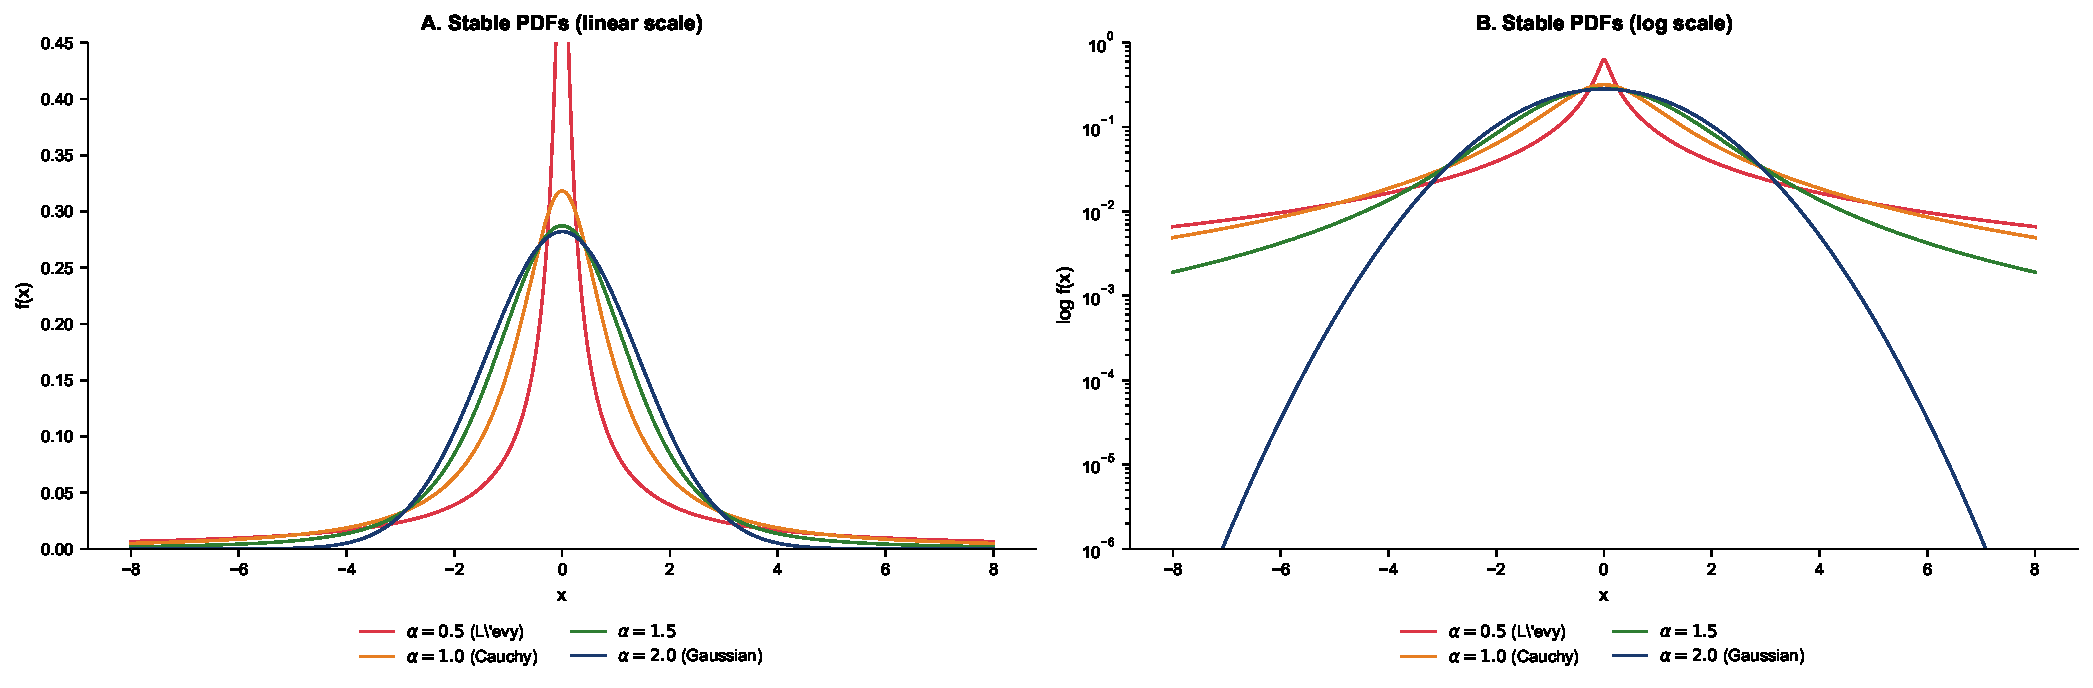
\includegraphics[width=\linewidth]{ch2_stable_pdfs.pdf}\\[0.2em]
\quantlet{SFM\_ch2}{https://github.com/QuantLet/Stat_fin_markets/tree/master/Quantlets/SFM_ch2}
\end{column}
\begin{column}{0.33\textwidth}
\begin{block}{Citirea graficului}
\begin{itemize}\setlength{\itemsep}{0pt}
    \item \textbf{Stânga (linear):} cu cât $\alpha$ scade, cu atât \emph{pic-ul} crește și se ascute
    \item \textbf{Dreapta (log):} cu cât $\alpha$ scade, cu atât \emph{cozile} sunt mai groase --- diferența e dramatică pe scară logaritmică
\end{itemize}
\end{block}
\begin{exampleblock}{Cazuri remarcabile}
\begin{itemize}\setlength{\itemsep}{0pt}
    \item $\alpha = 2$: Gaussian (cozi exponențiale)
    \item $\alpha = 1$: Cauchy (varianța deja $\infty$)
    \item $\alpha = 0{,}5$: Lévy (chiar și media $\infty$ pentru asimetrie totală)
\end{itemize}
\end{exampleblock}
\textit{Pentru BTC, $\hat\alpha \approx 1{,}5$ corespunde curbei verzi --- intermediar între Cauchy și Gaussian.}
\end{column}
\end{columns}
\end{cminipage}
\end{frame}

\begin{frame}[shrink=25]{Exercițiul 8: McCulloch cuantile și cozile grele}
\begin{cminipage}{0.95\textwidth}
\begin{block}{Enunț}
\begin{itemize}\setlength{\itemsep}{0pt}
    \item Cuantile empirice pe randamente Bitcoin:
    \begin{itemize}\setlength{\itemsep}{0pt}
        \item $q_{0{,}05} = -0{,}078$; $q_{0{,}25} = -0{,}018$
        \item $q_{0{,}75} = 0{,}020$; $q_{0{,}95} = 0{,}085$
    \end{itemize}
    \item Statistica McCulloch: $v_\alpha = (q_{0{,}95} - q_{0{,}05})/(q_{0{,}75} - q_{0{,}25})$
    \item \textbf{Cerințe:}
    \begin{itemize}\setlength{\itemsep}{0pt}
        \item Calculați $v_\alpha$
        \item Interpretați vs Normal ($\approx 2{,}44$) și Cauchy ($\approx 25$)
        \item Estimați $\alpha$ corespunzător (tabelat: $v_\alpha = 4{,}28 \Rightarrow \alpha \approx 1{,}5$)
        \item Avantajele McCulloch față de MLE
    \end{itemize}
\end{itemize}
\end{block}
\end{cminipage}
\end{frame}

\begin{frame}[shrink=25]{Exercițiul 8: Rezolvare}
\begin{cminipage}{0.95\textwidth}
\begin{exampleblock}{Rezolvare}
\begin{itemize}\setlength{\itemsep}{0pt}
    \item \textbf{1. Calcul $v_\alpha$} \quad $v_\alpha = \dfrac{q_{0{,}95} - q_{0{,}05}}{q_{0{,}75} - q_{0{,}25}}$
    \begin{itemize}\setlength{\itemsep}{0pt}
        \item Numărător: $0{,}085 - (-0{,}078) = 0{,}163$
        \item Numitor: $0{,}020 - (-0{,}018) = 0{,}038$
        \item $v_\alpha = 0{,}163/0{,}038 \approx \mathbf{4{,}29}$
    \end{itemize}
    \item \textbf{2. Interpretare poziție:}
    \begin{itemize}\setlength{\itemsep}{0pt}
        \item $4{,}29 \gg 2{,}44$ (normal) $\Rightarrow$ cozi \emph{semnificativ} mai grele
        \item $4{,}29 \ll 25$ (Cauchy) $\Rightarrow$ cozile \emph{nu} sunt extreme
        \item \textit{Interpretare:} BTC are cozi între Normal și Cauchy. Cuantilele extreme sunt $\sim 4\times$ mai mari decât intercuartilele --- semnătura unei distribuții cu varianță infinită
    \end{itemize}
    \item \textbf{3. Estimare $\alpha$} \quad tabelat: $v_\alpha = 4{,}3 \Rightarrow \hat\alpha \approx 1{,}5$
    \begin{itemize}\setlength{\itemsep}{0pt}
        \item Consecință: varianța \textbf{infinită}; momentele $p < 1{,}5$ finite
        \item \textit{Interpretare:} $\hat\alpha = 1{,}5$ înseamnă că modelul Black--Scholes (Gaussian) este complet inadecvat pentru BTC --- VaR Gaussian subestimează dramatic
    \end{itemize}
    \item \textbf{4. Avantajele McCulloch față de MLE:}
    \begin{itemize}\setlength{\itemsep}{0pt}
        \item Robust la outliers (cuantile, nu momente)
        \item $O(n)$ operații (sort); nu cere formă PDF
        \item Inițializare excelentă pentru MLE iterativ
        \item \textit{Interpretare:} densitatea stabilă nu are formă închisă; MLE e numeric și sensibil la inițializare. McCulloch dă o estimare rapidă, robustă, perfectă ca \emph{warm-start} pentru MLE
    \end{itemize}
\end{itemize}
\end{exampleblock}
\end{cminipage}
\end{frame}

%=============================================================================
% PARTEA IV: CAP.4 --- EMH
%=============================================================================
\section{Partea IV: Cap.~4 --- Ipoteza Pieței Eficiente}

\begin{frame}[shrink=25]{Exercițiul 9: Autocorelație și testul Ljung--Box}
\begin{cminipage}{0.95\textwidth}
\begin{block}{Enunț}
\begin{itemize}\setlength{\itemsep}{0pt}
    \item Eșantion $n = 250$ randamente zilnice:
    \begin{itemize}\setlength{\itemsep}{0pt}
        \item $\hat\rho_1 = 0{,}08$; $\hat\rho_2 = -0{,}05$; $\hat\rho_3 = 0{,}03$
        \item $\hat\rho_4 = 0{,}02$; $\hat\rho_5 = -0{,}06$
    \end{itemize}
    \item Formula statisticii Ljung--Box și ipoteza testată:
    \begin{itemize}\setlength{\itemsep}{0pt}
        \item $Q(m) = n(n+2)\sum_{k=1}^{m}\frac{\hat\rho_k^2}{n-k}$, unde sub $H_0$ avem $Q \sim \chi^2_m$
        \item $H_0$: toate autocorelațiile $\rho_1, \ldots, \rho_m$ sunt simultan zero
    \end{itemize}
    \item \textbf{Cerințe:}
    \begin{itemize}\setlength{\itemsep}{0pt}
        \item Calculați explicit valoarea statisticii $Q(5)$ pentru autocorelațiile date, detaliind fiecare termen al sumei
        \item Testați ipoteza nulă $H_0$ la pragul de semnificație $\alpha = 5\%$ folosind valoarea critică $\chi^2_5(0{,}05) = 11{,}07$ și formulați explicit decizia statistică
        \item Discutați dacă respingerea lui $H_0$ implică automat existența unei oportunități de profit exploatabile în trading; argumentați luând în considerare costurile de tranzacție și diferența esențială dintre semnificația statistică și cea economică
        \item Explicați legătura directă a testului Ljung--Box cu Ipoteza Pieței Eficiente în formă slabă: ce presupunere despre predictibilitatea randamentelor testează $Q(m)$ și cum interpretăm rezultatul obținut drept evidență în favoarea sau împotriva EMH slabe
    \end{itemize}
\end{itemize}
\end{block}
\end{cminipage}
\end{frame}

\begin{frame}[shrink=25]{Exercițiul 9: Rezolvare}
\begin{cminipage}{0.95\textwidth}
\begin{exampleblock}{Rezolvare}
\small
\begin{itemize}\setlength{\itemsep}{0pt}
    \item \textbf{1. Statistica Ljung--Box} \quad $Q(m) = n(n+2)\sum_{k=1}^{m}\dfrac{\hat\rho_k^2}{n-k} \xrightarrow{H_0} \chi^2_m$
    \begin{itemize}\setlength{\itemsep}{0pt}
        \item $n(n+2) = 63.000$
        \item $\rho_1^2/(n-1) = 0{,}0064/249 = 2{,}57 \cdot 10^{-5}$
        \item $\rho_2^2/(n-2) = 0{,}0025/248 = 1{,}01 \cdot 10^{-5}$
        \item $\rho_3^2/(n-3) = 0{,}0009/247 = 3{,}64 \cdot 10^{-6}$
        \item $\rho_4^2/(n-4) = 0{,}0004/246 = 1{,}63 \cdot 10^{-6}$
        \item $\rho_5^2/(n-5) = 0{,}0036/245 = 1{,}47 \cdot 10^{-5}$
    \end{itemize}
    \item \textbf{2. Calcul $Q(5)$:}
    \begin{itemize}\setlength{\itemsep}{0pt}
        \item Sumă $\approx 5{,}59 \cdot 10^{-5}$
        \item $Q(5) = 63.000 \cdot 5{,}59 \cdot 10^{-5} \approx \mathbf{3{,}52}$
    \end{itemize}
    \item \textbf{3. Decizia} \quad respingem $H_0$ dacă $Q(m) > \chi^2_m(\alpha)$
    \begin{itemize}\setlength{\itemsep}{0pt}
        \item $3{,}52 < 11{,}07 \Rightarrow$ nu respingem $H_0$
        \item Randamentele sunt compatibile cu necorelare
    \end{itemize}
    \item \textbf{4. Profit și EMH slabă:}
    \begin{itemize}\setlength{\itemsep}{0pt}
        \item Semnificație statistică $\neq$ semnificație economică
        \item Profit necesită depășirea costurilor de tranzacție (uzual $5$--$15$ bp/tranzacție)
        \item \textit{Interpretare:} chiar dacă am respinge $H_0$ cu $\hat\rho_1 = 0{,}05$, profit-ul așteptat per tranzacție ar fi $\sim 5$ bp --- sub costurile de execuție. Concluzie: necorelare $\Rightarrow$ EMH slabă plauzibilă
    \end{itemize}
\end{itemize}
\end{exampleblock}
\end{cminipage}
\end{frame}

\begin{frame}[shrink=25]{Exercițiul 10: Testul Runs și Variance Ratio}
\begin{cminipage}{0.95\textwidth}
\begin{block}{Enunț}
\begin{itemize}\setlength{\itemsep}{0pt}
    \item Secvența de semne a randamentelor:
    \begin{itemize}\setlength{\itemsep}{0pt}
        \item $+, +, -, +, -, -, +, -, +, +, -, +$
    \end{itemize}
    \item \textbf{Cerințe:}
    \begin{itemize}\setlength{\itemsep}{0pt}
        \item Numărați explicit $n_+$ (randamente pozitive), $n_-$ (negative), $n$ (total), apoi identificați grupurile consecutive de același semn și numărați runs-urile $R$
        \item Calculați speranța $\E[R] = \frac{2n_+n_-}{n}+1$ și varianța $\Var(R) = \frac{2n_+n_-(2n_+n_- - n)}{n^2(n-1)}$ sub ipoteza de independență a semnelor
        \item Construiți statistica standardizată $Z = (R - \E[R])/\sqrt{\Var(R)}$ și testați ipoteza $H_0$ de independență a semnelor la pragul $\alpha = 5\%$, folosind valoarea critică $z_{0{,}025} = 1{,}96$
        \item Pe aceleași date se obține $VR(2) = 0{,}72$; interpretați acest rezultat identificând dacă indică mean reversion ($VR < 1$) sau momentum ($VR > 1$) și explicați economic ce tip de dependență între randamente consecutive sugerează
    \end{itemize}
\end{itemize}
\end{block}
\end{cminipage}
\end{frame}

\begin{frame}[shrink=25]{Exercițiul 10: Rezolvare}
\begin{cminipage}{0.95\textwidth}
\begin{exampleblock}{Rezolvare}
\begin{itemize}\setlength{\itemsep}{0pt}
    \item \textbf{1. Numărare:}
    \begin{itemize}\setlength{\itemsep}{0pt}
        \item $n_+ = 7$, $n_- = 5$, $n = 12$
        \item Grupuri: $(++)(-)(+)(--)(+)(-)(++)(-)(+) \Rightarrow R = 9$
    \end{itemize}
    \item \textbf{2. Speranță și varianță} \quad $\E[R] = \dfrac{2n_+ n_-}{n} + 1$;\ $\Var(R) = \dfrac{2n_+n_-(2n_+n_- - n)}{n^2(n-1)}$
    \begin{itemize}\setlength{\itemsep}{0pt}
        \item $\E[R] = 2 \cdot 7 \cdot 5/12 + 1 = 6{,}833$
        \item $\Var(R) = 2 \cdot 35 \cdot 58/(144 \cdot 11) = 4.060/1.584 = 2{,}563$
        \item $\sqrt{\Var(R)} = 1{,}601$
    \end{itemize}
    \item \textbf{3. Statistica $Z$ și decizia} \quad $Z = (R - \E[R])/\sqrt{\Var(R)} \xrightarrow{H_0} \mathcal{N}(0,1)$
    \begin{itemize}\setlength{\itemsep}{0pt}
        \item $Z = (9 - 6{,}833)/1{,}601 = \mathbf{1{,}354}$
        \item $|Z| = 1{,}354 < 1{,}96 \Rightarrow$ nu respingem $H_0$ (semne independente)
    \end{itemize}
    \item \textbf{4. Interpretare $VR(2) = 0{,}72$} \quad $VR(q) = \sigma^2(q)/(q\sigma^2(1))$
    \begin{itemize}\setlength{\itemsep}{0pt}
        \item $VR < 1 \Rightarrow$ mean reversion (varianță $2$-periodică \emph{sub} dublu); $\hat\rho_1 = (VR(2)-1)/2 = -0{,}14$
        \item \textit{Interpretare:} mean reversion la $q = 2$ înseamnă că o creștere e urmată mai des de o scădere decât în RW. Posibilă strategie: short după zile pozitive, long după negative. Atenție: efectul e mic, costurile pot anula profitul
        \item Contrast: $VR > 1 \Rightarrow$ momentum;\ $VR = 1 \Rightarrow$ random walk pur
    \end{itemize}
\end{itemize}
\end{exampleblock}
\end{cminipage}
\end{frame}

\begin{frame}[shrink=25]{Exercițiul 11: Event Study --- CAR}
\begin{cminipage}{0.95\textwidth}
\begin{block}{Enunț}
\begin{itemize}\setlength{\itemsep}{0pt}
    \item Anunț financiar la $t = 0$, $AR_t$ (\%) pe fereastra $[-2, +3]$:
    \begin{itemize}\setlength{\itemsep}{0pt}
        \item $AR_{-2} = -0{,}1$; $AR_{-1} = 0{,}3$; $AR_0 = 2{,}5$
        \item $AR_{+1} = 0{,}8$; $AR_{+2} = -0{,}2$; $AR_{+3} = 0{,}1$
    \end{itemize}
    \item Deviație standard pe fereastra de estimare: $\hat\sigma_{AR} = 1{,}2\%$
    \item \textbf{Cerințe:}
    \begin{itemize}\setlength{\itemsep}{0pt}
        \item Calculați Cumulative Abnormal Return $CAR[-2, +3] = \sum_{t=-2}^{+3} AR_t$ ca sumă a abaterilor zilnice
        \item Testați ipoteza nulă $H_0: CAR = 0$ folosind statistica $t = CAR / (\hat\sigma_{AR}\sqrt{L})$, unde $L = 6$ este lungimea ferestrei, și comparați cu valoarea critică $1{,}96$
        \item Analizați profilul AR-urilor pre-eveniment ($AR_{-2}, AR_{-1}$) pentru a identifica dacă a existat o scurgere de informație înainte de anunț sau dacă reacția este o surpriză pură la $t = 0$
        \item Discutați legătura rezultatului cu Ipoteza Pieței Eficiente în formă semi-tare: o ajustare rapidă (1-2 zile) este compatibilă cu EMH semi-tare, iar un drift persistent post-eveniment (PEAD) contrazice EMH semi-tare
    \end{itemize}
\end{itemize}
\end{block}
\end{cminipage}
\end{frame}

\begin{frame}[shrink=25]{Exercițiul 11: Rezolvare}
\begin{cminipage}{0.95\textwidth}
\begin{exampleblock}{Rezolvare}
\begin{itemize}\setlength{\itemsep}{0pt}
    \item \textbf{1. CAR} \quad $CAR[t_1, t_2] = \sum_{t=t_1}^{t_2} AR_t$
    \begin{itemize}\setlength{\itemsep}{0pt}
        \item $CAR = -0{,}1 + 0{,}3 + 2{,}5 + 0{,}8 - 0{,}2 + 0{,}1 = \mathbf{3{,}4\%}$
    \end{itemize}
    \item \textbf{2. Testul $t$} \quad $t = CAR / (\hat\sigma_{AR}\sqrt{L})$
    \begin{itemize}\setlength{\itemsep}{0pt}
        \item $t = 3{,}4/(1{,}2 \cdot \sqrt{6}) = \mathbf{1{,}156}$;\ $|t| < 1{,}96 \Rightarrow$ nu respingem $H_0$
        \item \textit{Interpretare:} CAR $= 3{,}4\%$ pare mare, dar zgomotul ferestrei ($\sim 2{,}94$) este comparabil. Pe \emph{un} eveniment individual avem prea puțină putere; agregarea pe $N$ firme reduce $\Var(\overline{CAR})$ ca $1/N$
    \end{itemize}
    \item \textbf{3. Diagnostic scurgere:}
    \begin{itemize}\setlength{\itemsep}{0pt}
        \item $AR_{-2}, AR_{-1}$ mici $\Rightarrow$ \textbf{nu există scurgere}
        \item Salt $+2{,}5\%$ la $t = 0$, $+0{,}8\%$ la $t = +1$ $\Rightarrow$ surpriză pură
        \item \textit{Interpretare:} dacă pre-eveniment $CAR > 0$ pe mai multe firme, ar fi suspect de \emph{insider trading}; aici pattern-ul este curat
    \end{itemize}
    \item \textbf{4. EMH semi-tare:}
    \begin{itemize}\setlength{\itemsep}{0pt}
        \item Ajustare rapidă la info publică $\Rightarrow$ compatibil cu EMH semi-tare
        \item Dacă $AR > 0$ ar continua 5+ zile (PEAD) $\Rightarrow$ evidență contra
        \item \textit{Interpretare:} pattern-ul ``jump la $t = 0$ + decay rapid'' este manualul EMH; PEAD (Bernard \& Thomas 1989) este anomalia majoră
    \end{itemize}
\end{itemize}
\end{exampleblock}
\end{cminipage}
\end{frame}

\begin{frame}[shrink=25]{Exercițiul 12: Exponentul Hurst}
\begin{cminipage}{0.95\textwidth}
\begin{block}{Enunț}
\begin{itemize}\setlength{\itemsep}{0pt}
    \item Trei active cu $\hat H$ estimat prin R/S:
    \begin{itemize}\setlength{\itemsep}{0pt}
        \item S\&P~500: $\hat H = 0{,}52$
        \item Bitcoin: $\hat H = 0{,}62$
        \item Pairs trading: $\hat H = 0{,}38$
    \end{itemize}
    \item \textbf{Cerințe:}
    \begin{itemize}\setlength{\itemsep}{0pt}
        \item Interpretați economic fiecare valoare $\hat H$ estimată, identificând dacă indică memorie lungă, random walk sau mean reversion, și explicați ce înseamnă fiecare pentru comportamentul seriei
        \item Specificați explicit ce valoare a exponentului Hurst $H$ corespunde random walk-ului pur și ce implică această valoare pentru ipoteza de eficiență
        \item Explicați relația asimptotică dintre exponentul Hurst și variance ratio: $VR(q) \sim q^{2H-1}$, și discutați cum se traduce $H > 0{,}5$ sau $H < 0{,}5$ în comportamentul $VR$
        \item Încadrați rezultatele observate în contextul Adaptive Markets Hypothesis (Lo, 2004): cum explică AMH faptul că eficiența variază între active și în timp, în funcție de lichiditate și maturitatea pieței
    \end{itemize}
\end{itemize}
\end{block}
\end{cminipage}
\end{frame}

\begin{frame}[shrink=25]{Exercițiul 12: Rezolvare}
\begin{cminipage}{0.95\textwidth}
\begin{exampleblock}{Rezolvare}
\begin{itemize}\setlength{\itemsep}{0pt}
    \item \textbf{1. Interpretare pe activ:}
    \begin{itemize}\setlength{\itemsep}{0pt}
        \item S\&P~500 ($H = 0{,}52$): cvasi random walk, foarte aproape de eficiența perfectă
        \item Bitcoin ($H = 0{,}62$): memorie lungă, tendințe persistente exploatabile
        \item Pairs trading ($H = 0{,}38$): mean reversion construit prin design
        \item \textit{Interpretare:} valorile semnalează \emph{regimul} pieței. SPY e ``aproape RW''; BTC are tendințe lungi (lipsă lichiditate, jucători retail dominanți); pairs trading e construit \emph{deliberat} să fie anti-persistent
    \end{itemize}
    \item \textbf{2. Random walk pur:} $H = 0{,}5$ $\Leftrightarrow$ varianță proporțională cu $T$
    \begin{itemize}\setlength{\itemsep}{0pt}
        \item \textit{Interpretare:} $H = 0{,}5$ este punctul de echilibru. În practică $|H - 0{,}5| < 0{,}05$ este indistinguibil de RW pe eșantioane finite (precizia $\hat H \approx 0{,}03$ pe $n = 1000$)
    \end{itemize}
    \item \textbf{3. Relația $H \leftrightarrow VR$} \quad asimptotic $VR(q) \sim q^{2H-1}$
    \begin{itemize}\setlength{\itemsep}{0pt}
        \item $H > 0{,}5 \Rightarrow VR(q) > 1$ (momentum);\ $H < 0{,}5 \Rightarrow VR(q) < 1$ (mean reversion)
        \item \textit{Interpretare:} $H$ și $VR$ sunt \emph{două măsuri ale aceleiași proprietăți}: cum se scaleze varianța sumelor cu orizontul. Concordanța lor e o verificare cross-check
    \end{itemize}
    \item \textbf{4. Integrare AMH (Lo, 2004):}
    \begin{itemize}\setlength{\itemsep}{0pt}
        \item Eficiența variază cu lichiditatea, maturitatea, numărul de arbitragiști
        \item BTC (tânăr) $<$ eficient decât S\&P~500 (matur, lichid, sub Reg.\ NMS)
        \item \textit{Interpretare:} AMH explică de ce $\hat H$ \emph{variază în timp} pentru același activ --- piețele evoluează ca ecosisteme; ineficiențele se ``epuizează'' pe măsură ce sunt arbitrate
    \end{itemize}
\end{itemize}
\end{exampleblock}
\end{cminipage}
\end{frame}

%=============================================================================
% PARTEA V: CAP.~10 --- IPOTEZA PIEȚEI FRACTALE (FMH)
%=============================================================================
\section{Partea V: Cap.~5 --- Ipoteza Pieței Fractale (FMH)}

\begin{frame}[shrink=25]{FMH --- recap teoretic în 1 slide}
\begin{cminipage}{0.95\textwidth}
\begin{columns}[T]
\begin{column}{0.55\textwidth}
\begin{block}{Cei 3 piloni Peters (1991, 1994)}
\begin{enumerate}\setlength{\itemsep}{0pt}
    \item \textbf{Eterogenitatea orizonturilor de investiție}: traderi intraday, săptămânali, manageri lunari/anuali coexistă $\Rightarrow$ piața lichidă \emph{atunci} când orizonturile sunt diverse
    \item \textbf{Informația este interpretată diferit pe fiecare orizont}: o știre macro contează altfel pentru un HFT vs.\ un fond de pensii
    \item \textbf{Crizele apar când orizonturile colapsează la unul singur} (panică, lichiditate evaporată)
\end{enumerate}
\end{block}
\begin{exampleblock}{EMH vs FMH}
\begin{itemize}\setlength{\itemsep}{0pt}
    \item EMH: agent reprezentativ, i.i.d., Gaussian, $\sqrt T$
    \item FMH: orizonturi multiple, memorie lungă, autosimilaritate, $T^H$
\end{itemize}
\end{exampleblock}
\end{column}
\begin{column}{0.42\textwidth}
\begin{alertblock}{Formule cheie}
\begin{itemize}\setlength{\itemsep}{0pt}
    \item Dimensiune fractală: $D = 2 - H$
    \item $H = 0{,}5$: random walk (sub EMH)
    \item $H > 0{,}5$: persistență (memorie lungă pozitivă)
    \item $H < 0{,}5$: anti-persistență (mean-reversion)
    \item Scalarea varianței: $\Var(r_T) \propto T^{2H}$
    \item Scalarea VaR: $\text{VaR}_T \approx \text{VaR}_1 \cdot T^H$ (\textbf{nu} $\sqrt T$ când $H \neq 0{,}5$)
\end{itemize}
\end{alertblock}
\end{column}
\end{columns}
\end{cminipage}
\end{frame}

\begin{frame}[shrink=25]{Exercițiul F1: Dimensiunea fractală a unor mulțimi clasice}
\begin{cminipage}{0.95\textwidth}
\begin{block}{Enunț}
\begin{itemize}\setlength{\itemsep}{0pt}
    \item Pentru o mulțime autosimilară compusă din $N$ copii la scară $1/s$, dimensiunea fractală (similaritate) este
    $D = \dfrac{\ln N}{\ln s}$
    \item Calculați $D$ pentru:
    \begin{enumerate}\setlength{\itemsep}{0pt}
        \item Mulțimea Cantor: $N = 2$, $s = 3$
        \item Curba Koch: $N = 4$, $s = 3$
        \item Triunghiul Sierpinski: $N = 3$, $s = 2$
        \item Buretele Menger 3D: $N = 20$, $s = 3$
    \end{enumerate}
    \item Pentru o serie de prețuri cu $\hat H = 0{,}62$, calculați $D$ corespunzător și interpretați
\end{itemize}
\end{block}
\end{cminipage}
\end{frame}

\begin{frame}[shrink=25]{Exercițiul F1: Rezolvare}
\begin{cminipage}{0.95\textwidth}
\begin{exampleblock}{Rezolvare}
\begin{itemize}\setlength{\itemsep}{0pt}
    \item \textbf{Cantor}: $D = \ln 2 / \ln 3 \approx \mathbf{0{,}631}$ \quad (între punct și segment)
    \item \textbf{Koch}: $D = \ln 4 / \ln 3 \approx \mathbf{1{,}262}$ \quad (între curbă și suprafață)
    \item \textbf{Sierpinski}: $D = \ln 3 / \ln 2 \approx \mathbf{1{,}585}$
    \item \textbf{Menger}: $D = \ln 20 / \ln 3 \approx \mathbf{2{,}727}$ \quad (între suprafață și volum)
    \item \textbf{Serie cu $\hat H = 0{,}62$}: $D = 2 - 0{,}62 = \mathbf{1{,}38}$
    \begin{itemize}\setlength{\itemsep}{0pt}
        \item $D < 1{,}5$ $\Rightarrow$ traiectoria este \emph{mai netedă} decât random walk
        \item Persistență: tendințele se mențin pe orizonturi multiple
    \end{itemize}
\end{itemize}
\end{exampleblock}
\begin{block}{De reținut}
\begin{itemize}\setlength{\itemsep}{0pt}
    \item Pentru obiecte autosimilare clasice, $D$ este non-întreg --- semnătura fractalității
    \item Pentru serii temporale: $D = 2 - H$, $D \in [1, 2]$
\end{itemize}
\end{block}
\end{cminipage}
\end{frame}

\begin{frame}[shrink=25]{Exercițiul F2: Algoritmul R/S pas-cu-pas}
\begin{cminipage}{0.95\textwidth}
\begin{block}{Enunț}
\begin{itemize}\setlength{\itemsep}{0pt}
    \item Se dau 8 randamente: $r = (0{,}02, -0{,}01, 0{,}03, 0{,}00, -0{,}02, 0{,}01, 0{,}02, -0{,}01)$
    \item \textbf{Cerințe:}
    \begin{enumerate}\setlength{\itemsep}{0pt}
        \item Calculați media $\bar r$ și abaterile centrate $y_t = r_t - \bar r$
        \item Calculați seria deviațiilor cumulative $Y_t = \sum_{i=1}^t y_i$
        \item Calculați range-ul $R = \max_t Y_t - \min_t Y_t$ și abaterea standard $S$
        \item Raportați $R/S$ și discutați ce se obține pe sub-eșantioane succesive
        \item Explicați \emph{pe scurt} cum estimați $\hat H$ din regresia $\ln(R/S) = \ln c + H \ln n$
    \end{enumerate}
\end{itemize}
\end{block}
\end{cminipage}
\end{frame}

\begin{frame}[shrink=25]{Exercițiul F2: Rezolvare}
\begin{cminipage}{0.95\textwidth}
\begin{exampleblock}{Rezolvare}
\small
\begin{itemize}\setlength{\itemsep}{0pt}
    \item \textbf{1. Media:} $\bar r = 0{,}04/8 = 0{,}005$
    \item \textbf{2. Abateri centrate $y_t$:}
    \begin{itemize}\setlength{\itemsep}{0pt}
        \item $0{,}015,\ -0{,}015,\ 0{,}025,\ -0{,}005,\ -0{,}025,\ 0{,}005,\ 0{,}015,\ -0{,}015$
    \end{itemize}
    \item \textbf{3. Cumulate $Y_t$:}
    \begin{itemize}\setlength{\itemsep}{0pt}
        \item $0{,}015,\ 0{,}000,\ 0{,}025,\ 0{,}020,\ -0{,}005,\ 0{,}000,\ 0{,}015,\ 0{,}000$
    \end{itemize}
    \item \textbf{4. Range și std:}
    \begin{itemize}\setlength{\itemsep}{0pt}
        \item $R = \max Y_t - \min Y_t = 0{,}025 - (-0{,}005) = 0{,}030$
        \item $S = \sqrt{\frac{1}{8}\sum y_t^2} \approx 0{,}01658$
        \item $R/S \approx 0{,}030/0{,}01658 \approx \mathbf{1{,}81}$
    \end{itemize}
    \item \textbf{5. Estimarea $\hat H$:} Se împarte seria în sub-eșantioane de lungimi $n$ diferite, se calculează $R/S$ mediu, apoi $\hat H$ = panta regresiei OLS a $\ln(R/S)$ pe $\ln n$
\end{itemize}
\end{exampleblock}
\begin{alertblock}{Atenție}
R/S clasic e \emph{biased} pe eșantioane mici și sub heteroskedasticitate $\Rightarrow$ folosiți \textbf{R/S Lo (1991)} sau \textbf{DFA} pe date reale
\end{alertblock}
\end{cminipage}
\end{frame}

\begin{frame}[shrink=25]{Exercițiul F3: Interpretarea $\hat H$ pe active reale}
\begin{cminipage}{0.95\textwidth}
\begin{block}{Enunț --- estimări $\hat H$ (R/S corectat) pe randamente zilnice}
\small
\renewcommand{\arraystretch}{1.2}
\begin{center}
\begin{tabular}{lccl}
\toprule
\textbf{Activ} & $\hat H$ & $D = 2 - \hat H$ & \textbf{Diagnostic} \\
\midrule
S\&P 500 (SPY) & $0{,}52$ & $1{,}48$ & ? \\
BET (BVB) & $0{,}63$ & $1{,}37$ & ? \\
Bitcoin (BTC) & $0{,}58$ & $1{,}42$ & ? \\
EUR/USD & $0{,}48$ & $1{,}52$ & ? \\
Volatilitate VIX & $0{,}82$ & $1{,}18$ & ? \\
\bottomrule
\end{tabular}
\end{center}
\end{block}
\begin{itemize}\setlength{\itemsep}{0pt}
    \item \textbf{Cerințe:} pentru fiecare activ, completați \emph{Diagnostic} (random walk / persistent / anti-persistent / memorie lungă) și interpretați practic. Comparați piețele dezvoltate cu BVB. De ce $\hat H_{\text{VIX}} \gg 0{,}5$?
\end{itemize}
\end{cminipage}
\end{frame}

\begin{frame}[shrink=25]{Exercițiul F3: Rezolvare}
\begin{cminipage}{0.95\textwidth}
\begin{exampleblock}{Rezolvare}
\begin{itemize}\setlength{\itemsep}{0pt}
    \item \textbf{S\&P 500 ($\hat H = 0{,}52$):} foarte aproape de RW $\Rightarrow$ piață \textbf{aproape eficientă} (compatibil EMH slabă). $D \approx 1{,}48 \approx 1{,}5$
    \item \textbf{BET ($\hat H = 0{,}63$):} \textbf{persistent} $\Rightarrow$ tendințele se prelungesc; semn de eficiență mai slabă (piață emergentă, lichiditate redusă, free-float mic). Strategii de momentum pot funcționa
    \item \textbf{BTC ($\hat H = 0{,}58$):} ușoară persistență, dar atenție: $\hat H$ poate fi inflat de bule și jumps; combinați cu DFA și sub-eșantioane mobile
    \item \textbf{EUR/USD ($\hat H = 0{,}48$):} \textbf{anti-persistent} ușor $\Rightarrow$ mean-reversion (semn al activității market-makerilor și triangulare FX)
    \item \textbf{VIX ($\hat H = 0{,}82$):} \textbf{memorie lungă puternică} $\Rightarrow$ volatilitatea persistă (motivează FIGARCH, rough volatility, regimuri de volatilitate)
\end{itemize}
\end{exampleblock}
\begin{block}{Concluzie}
Piețele dezvoltate sunt aproape de $H = 0{,}5$; emergente (BVB, cripto) tind la persistență; volatilitatea (nu randamentul!) are memorie lungă pe toate piețele.
\end{block}
\end{cminipage}
\end{frame}

\begin{frame}[shrink=25]{Exercițiul F4: Scalarea VaR --- $\sqrt T$ vs $T^H$}
\begin{cminipage}{0.95\textwidth}
\begin{block}{Enunț}
\begin{itemize}\setlength{\itemsep}{0pt}
    \item Un portofoliu are VaR zilnic $\text{VaR}_1 = 1\%$ la nivelul $99\%$
    \item Estimări: $\hat\sigma_{\text{zi}} = 1\%$, $\hat H = 0{,}62$
    \item \textbf{Cerințe:}
    \begin{enumerate}\setlength{\itemsep}{0pt}
        \item Calculați VaR pe orizont $T = 10$ zile sub regula clasică i.i.d. ($\sqrt T$)
        \item Recalculați-l sub scalarea fractală $T^{\hat H}$
        \item Calculați raportul și interpretați diferența
        \item Aceeași analiză pentru $\hat H = 0{,}40$ (anti-persistent)
        \item Discutați limitele practice: este $T^H$ scalarea standard în Basel?
    \end{enumerate}
\end{itemize}
\end{block}
\end{cminipage}
\end{frame}

\begin{frame}[shrink=25]{Exercițiul F4: Rezolvare}
\begin{cminipage}{0.95\textwidth}
\begin{exampleblock}{Rezolvare}
\begin{itemize}\setlength{\itemsep}{0pt}
    \item \textbf{1. Sub $\sqrt T$:}
    \begin{itemize}\setlength{\itemsep}{0pt}
        \item $\text{VaR}_{10}^{\sqrt{}} = 1\% \cdot \sqrt{10} \approx \mathbf{3{,}16\%}$
    \end{itemize}
    \item \textbf{2. Sub $T^H$ cu $H = 0{,}62$:}
    \begin{itemize}\setlength{\itemsep}{0pt}
        \item $\text{VaR}_{10}^{H} = 1\% \cdot 10^{0{,}62} \approx 1\% \cdot 4{,}17 \approx \mathbf{4{,}17\%}$
    \end{itemize}
    \item \textbf{3. Raport:} $4{,}17/3{,}16 \approx 1{,}32$ $\Rightarrow$ \textbf{subestimare cu $\sim 32\%$} a riscului sub $\sqrt T$ pentru o piață persistentă
    \item \textbf{4. Sub $T^H$ cu $H = 0{,}40$ (anti-persistent):}
    \begin{itemize}\setlength{\itemsep}{0pt}
        \item $\text{VaR}_{10}^H = 1\% \cdot 10^{0{,}40} \approx \mathbf{2{,}51\%}$
        \item Sub $\sqrt T$ am \emph{supraestima} riscul cu $\sim 26\%$
    \end{itemize}
    \item \textbf{5. Limite practice:}
    \begin{itemize}\setlength{\itemsep}{0pt}
        \item Basel III/FRTB folosește scalarea standard ($\sqrt T$) pentru SRC + ES
        \item $T^H$ este util ca \textbf{stress-test} și \emph{senzitivitate}, nu ca substitut regulamentar
    \end{itemize}
\end{itemize}
\end{exampleblock}
\end{cminipage}
\end{frame}

\begin{frame}[shrink=25]{Exercițiul F5: $\hat H_t$ mobil ca semnal de criză}
\begin{cminipage}{0.95\textwidth}
\begin{block}{Enunț --- $\hat H$ rolling pe ferestre de 252 zile, S\&P 500, 1985--2022}
\begin{itemize}\setlength{\itemsep}{0pt}
    \item Valori observate ale $\hat H_t$ în jurul unor evenimente:
    \begin{itemize}\setlength{\itemsep}{0pt}
        \item Pre-octombrie 1987: $\hat H_t \approx 0{,}65$, ulterior $\to 0{,}48$
        \item Pre-2008 (mid-2007): $\hat H_t \approx 0{,}62$, ulterior $\to 0{,}45$
        \item Pre-COVID (ianuarie 2020): $\hat H_t \approx 0{,}60$, ulterior $\to 0{,}43$
    \end{itemize}
    \item \textbf{Cerințe:}
    \begin{enumerate}\setlength{\itemsep}{0pt}
        \item Ce semnifică o trecere bruscă de la $\hat H_t > 0{,}5$ la $\hat H_t < 0{,}5$?
        \item Cum se leagă această trecere de pilonul 3 al lui Peters (colaps al orizonturilor)?
        \item Poate $\hat H_t$ să fie folosit drept \emph{semnal de avertizare timpurie}? Avantaje și capcane (false signals, lookback bias).
    \end{enumerate}
\end{itemize}
\end{block}
\end{cminipage}
\end{frame}

\begin{frame}[shrink=25]{Exercițiul F5: Rezolvare}
\begin{cminipage}{0.95\textwidth}
\begin{exampleblock}{Rezolvare}
\begin{itemize}\setlength{\itemsep}{0pt}
    \item \textbf{1. Trecerea $\hat H_t > 0{,}5 \to < 0{,}5$:}
    \begin{itemize}\setlength{\itemsep}{0pt}
        \item Persistență (tendințe lungi) $\to$ anti-persistență (oscilații rapide)
        \item Reflectă schimbarea de regim: comportament dezordonat, panică, lichiditate fragilă
    \end{itemize}
    \item \textbf{2. Legătura cu pilonul 3 Peters:}
    \begin{itemize}\setlength{\itemsep}{0pt}
        \item Toți participanții acționează pe \emph{același} orizont scurt (lichiditate de urgență)
        \item Eterogenitatea orizonturilor se prăbușește $\Rightarrow$ piața nu mai e ``stabilă fractal''
        \item Empiric: $\hat H_t$ scade brusc înainte și în timpul crizelor
    \end{itemize}
    \item \textbf{3. $\hat H_t$ ca early-warning:}
    \begin{itemize}\setlength{\itemsep}{0pt}
        \item \textbf{Avantaje:} indicator continuu, model-free; corelat cu dispersia orizonturilor
        \item \textbf{Capcane:} fereastra de 252 zile = lookback bias; semnale false la zgomot temporar; $\hat H_t$ nu prezice \emph{cauza} crizei, doar regimul fractal
        \item Recomandare: combinați cu indicatori complementari (volatility regime, ACF, $\beta$ time-varying)
    \end{itemize}
\end{itemize}
\end{exampleblock}
\end{cminipage}
\end{frame}

\begin{frame}[shrink=25]{FMH --- Mini-glosar}
\begin{cminipage}{0.95\textwidth}
\begin{columns}[T]
\begin{column}{0.48\textwidth}
\begin{block}{Concepte fundamentale}
\begin{itemize}\setlength{\itemsep}{0pt}
    \item \textbf{Autosimilaritate (statistică)}: $X(\lambda t) \stackrel{d}{=} \lambda^H X(t)$
    \item \textbf{Dimensiune fractală}: $D = \ln N / \ln s$ (similaritate); pentru serii: $D = 2 - H$
    \item \textbf{Exponent Hurst $H$}: $\Var(r_T) \propto T^{2H}$
    \begin{itemize}\setlength{\itemsep}{0pt}
        \item $H=0{,}5$: random walk
        \item $H>0{,}5$: persistent
        \item $H<0{,}5$: anti-persistent
    \end{itemize}
    \item \textbf{R/S}: rescaled range, Hurst (1951), Nilul
    \item \textbf{Lo (1991)}: corecție pentru autocorelație și heteroskedasticitate
    \item \textbf{DFA}: detrended fluctuation analysis (Peng et al.\ 1994)
\end{itemize}
\end{block}
\end{column}
\begin{column}{0.48\textwidth}
\begin{block}{Modele și aplicații}
\begin{itemize}\setlength{\itemsep}{0pt}
    \item \textbf{fBm}: mișcare browniană fracționară (Mandelbrot--Van Ness, 1968)
    \item \textbf{ARFIMA}: AR fracționar integrat MA --- $(1-L)^d$, $d = H - 0{,}5$
    \item \textbf{Multifractalitate}: spectru $f(\alpha)$, MMAR, MFDFA
    \item \textbf{FIGARCH}: GARCH cu memorie lungă în volatilitate
    \item \textbf{Rough volatility}: $H \in (0, 0{,}5)$ pentru log-vol (Gatheral et al.\ 2018)
    \item \textbf{Cei 3 piloni Peters}: orizonturi multiple, interpretare diferențiată, colaps în criză
\end{itemize}
\end{block}
\end{column}
\end{columns}
\end{cminipage}
\end{frame}

%=============================================================================
% FMH GRAFICE
%=============================================================================
\begin{frame}[shrink=25]{Exercițiul F6: identificare fractali clasici}
\begin{cminipage}{0.95\textwidth}
\begin{columns}[T]
\begin{column}{0.32\textwidth}
\centering
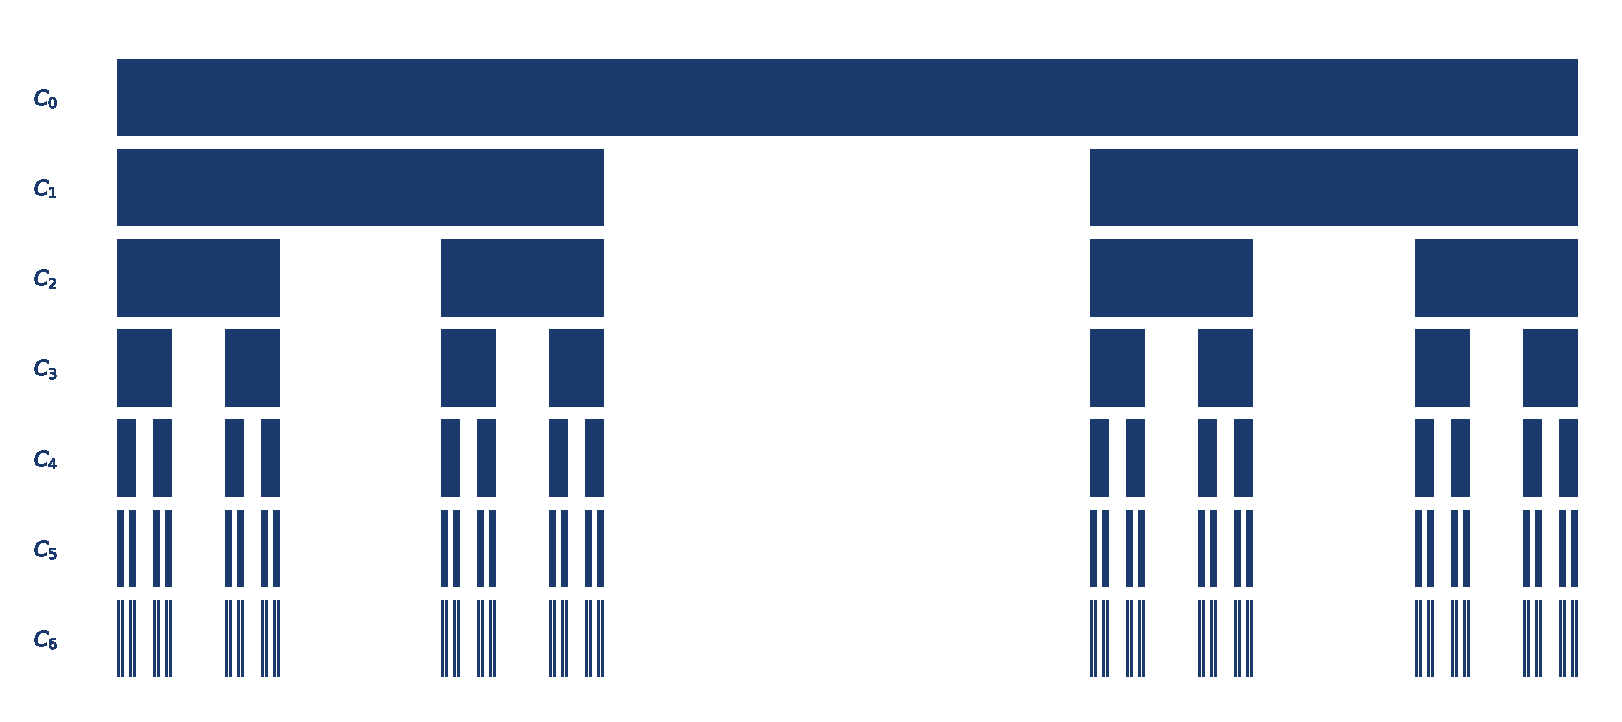
\includegraphics[width=\linewidth]{ch_fmh_cantor.pdf}\\[0.2em]
{\scriptsize Mulțimea Cantor}
\end{column}
\begin{column}{0.32\textwidth}
\centering
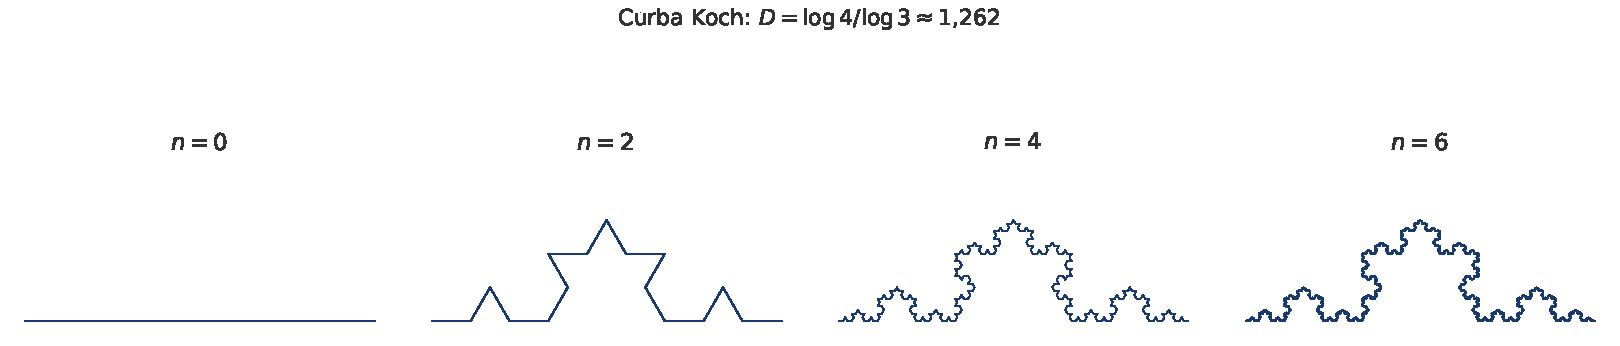
\includegraphics[width=\linewidth]{ch_fmh_koch_curve.pdf}\\[0.2em]
{\scriptsize Curba Koch}
\end{column}
\begin{column}{0.32\textwidth}
\centering
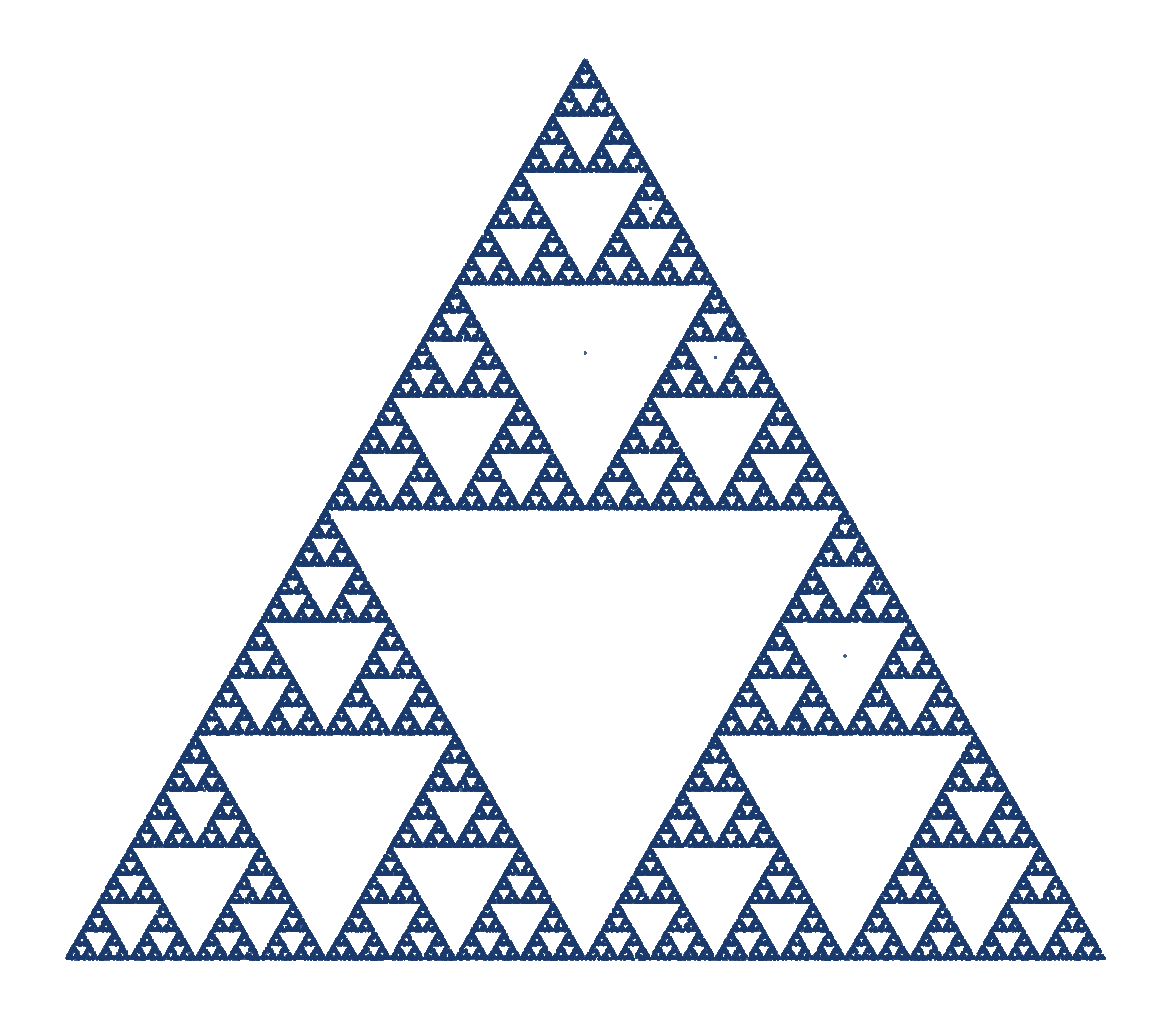
\includegraphics[width=\linewidth]{ch_fmh_sierpinski.pdf}\\[0.2em]
{\scriptsize Triunghiul Sierpinski}
\end{column}
\end{columns}
\vspace{0.1cm}
\quantlet{SFM\_ch\_fmh\_fractals}{https://github.com/QuantLet/Stat_fin_markets/tree/master/Quantlets/SFM_ch_fmh/SFM_ch_fmh_fractals}
\vspace{0.1cm}
\begin{block}{Cerințe}
\begin{itemize}\setlength{\itemsep}{0pt}
    \item Pentru fiecare obiect, identificați $N$ (copii la pasul de iterație) și $s$ (scara de reducere)
    \item Calculați dimensiunea fractală $D = \ln N / \ln s$
    \item Care obiect este ``cel mai apropiat'' de o suprafață? Care de un punct? Justificați
    \item Ce dimensiune topologică au cele trei obiecte? (Răspuns: 0, 1, 1.) Comparați cu $D$ fractală
\end{itemize}
\end{block}
\end{cminipage}
\end{frame}

\begin{frame}[shrink=25]{Exercițiul F6: Rezolvare}
\begin{cminipage}{0.95\textwidth}
\begin{exampleblock}{Rezolvare}
\begin{itemize}\setlength{\itemsep}{0pt}
    \item \textbf{Cantor}: $N = 2$, $s = 3$ $\Rightarrow$ $D = \ln 2 / \ln 3 \approx 0{,}631$
    \begin{itemize}\setlength{\itemsep}{0pt}
        \item Cel mai aproape de un \emph{punct} ($D < 1$); dimensiune topologică $0$
    \end{itemize}
    \item \textbf{Koch}: $N = 4$, $s = 3$ $\Rightarrow$ $D = \ln 4 / \ln 3 \approx 1{,}262$
    \begin{itemize}\setlength{\itemsep}{0pt}
        \item Curbă mai ``zimțată'' decât una netedă; dimensiune topologică $1$
    \end{itemize}
    \item \textbf{Sierpinski}: $N = 3$, $s = 2$ $\Rightarrow$ $D = \ln 3 / \ln 2 \approx 1{,}585$
    \begin{itemize}\setlength{\itemsep}{0pt}
        \item Cel mai aproape de o \emph{suprafață} ($D \to 2$); dimensiune topologică $1$
    \end{itemize}
\end{itemize}
\end{exampleblock}
\begin{block}{Observație fundamentală}
Pentru toate trei: $D > $ dimensiunea topologică $\Rightarrow$ semnătura tipică a fractalilor (Mandelbrot, 1982).
\end{block}
\end{cminipage}
\end{frame}

\begin{frame}[shrink=25]{Exercițiul F7: traiectorii fBm pentru $H \in \{0{,}3, 0{,}5, 0{,}7\}$}
\begin{cminipage}{0.95\textwidth}
\begin{columns}[T]
\begin{column}{0.6\textwidth}
\centering
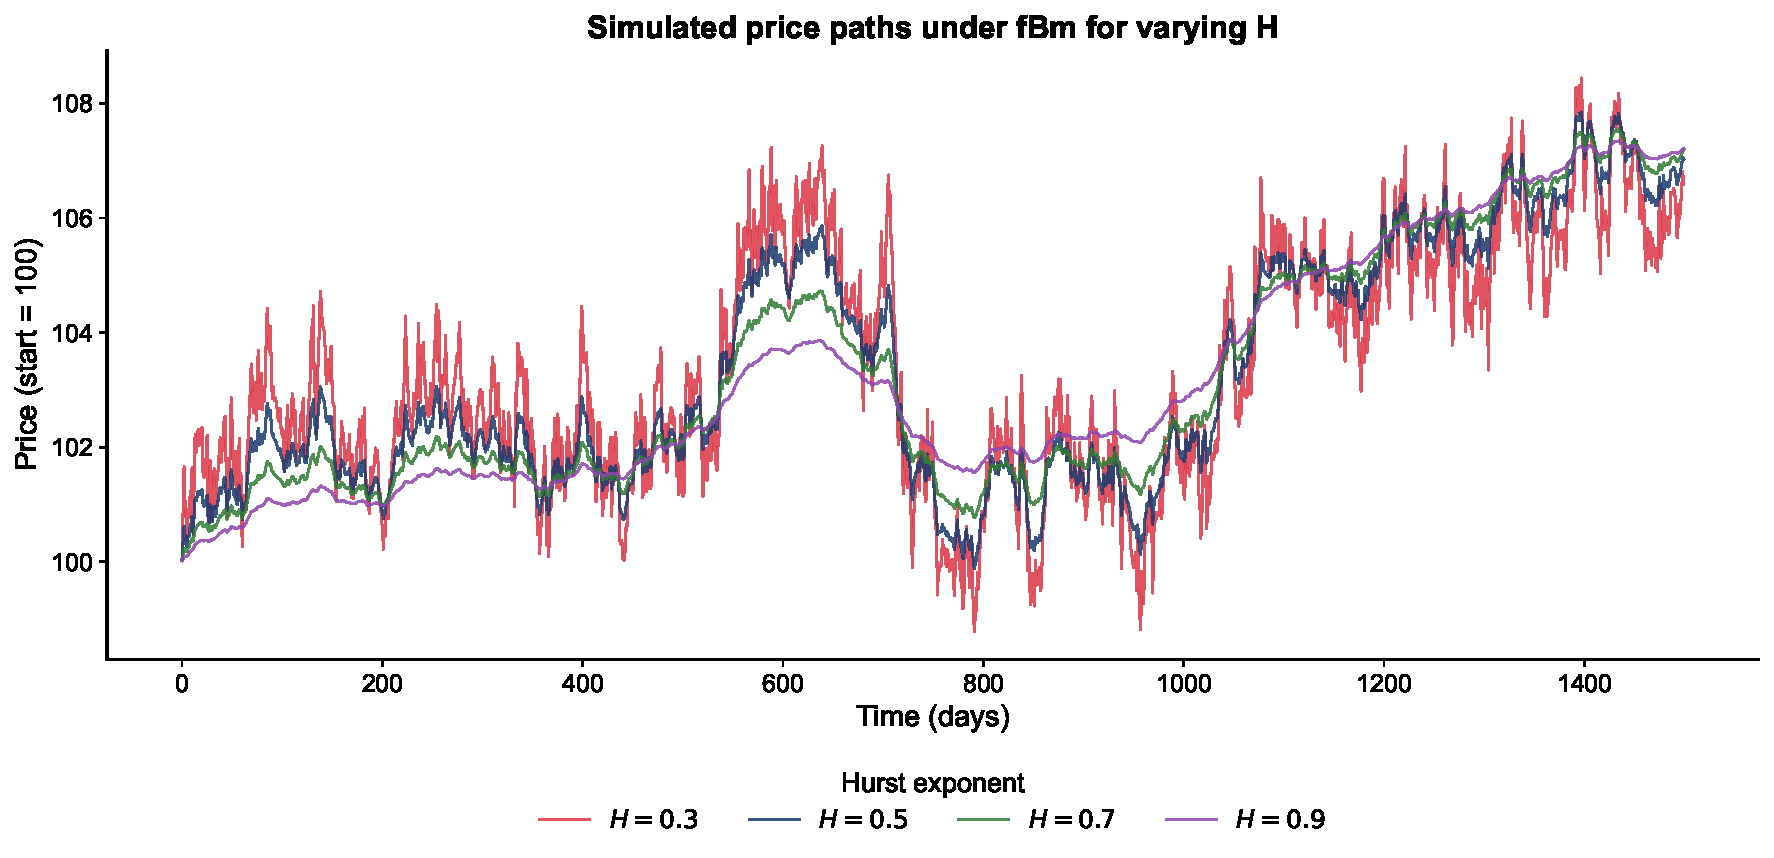
\includegraphics[width=\linewidth]{ch_fmh_price_paths_H.pdf}\\[0.2em]
\quantlet{SFM\_ch\_fmh\_extra}{https://github.com/QuantLet/Stat_fin_markets/tree/master/Quantlets/SFM_ch_fmh/SFM_ch_fmh_extra}
\end{column}
\begin{column}{0.37\textwidth}
\begin{block}{Cerințe}
\begin{itemize}\setlength{\itemsep}{0pt}
    \item Asociați fiecare traiectorie cu un $H$
    \item Care prezintă oscilații rapide (anti-persistent)?
    \item Care prezintă tendințe lungi (persistent)?
    \item Care este compatibilă cu RW?
    \item Calculați $D$ pentru fiecare
    \item Pe care piață realistă întâlniți $H \approx 0{,}3$? Dar $H \approx 0{,}7$?
\end{itemize}
\end{block}
\end{column}
\end{columns}
\end{cminipage}
\end{frame}

\begin{frame}[shrink=25]{Exercițiul F7: Rezolvare}
\begin{cminipage}{0.95\textwidth}
\begin{exampleblock}{Rezolvare}
\begin{itemize}\setlength{\itemsep}{0pt}
    \item \textbf{$H = 0{,}3$ (anti-persistent):} traiectorie ``zimțată'', oscilații rapide; $D = 1{,}7$
    \begin{itemize}\setlength{\itemsep}{0pt}
        \item Tipic: rate de schimb majore (EUR/USD intra-zilnic), spread-uri bid-ask, log-volatilitate (rough volatility, Gatheral et al.\ 2018)
    \end{itemize}
    \item \textbf{$H = 0{,}5$ (random walk):} fluctuații independente, fără tendințe; $D = 1{,}5$
    \begin{itemize}\setlength{\itemsep}{0pt}
        \item Tipic: indicii dezvoltați (S\&P 500, FTSE) pe orizont mediu/lung
    \end{itemize}
    \item \textbf{$H = 0{,}7$ (persistent):} tendințe lungi, ``netedă'' vizual; $D = 1{,}3$
    \begin{itemize}\setlength{\itemsep}{0pt}
        \item Tipic: piețe emergente (BVB), cripto pe ferestre cu bule, volatilitate (clustering); debit hidrologic (Nilul, Hurst 1951)
    \end{itemize}
\end{itemize}
\end{exampleblock}
\begin{alertblock}{De ce conteză}
Modelul i.i.d. ($H = 0{,}5$) este o \emph{idealizare}; pe date reale $\hat H$ rareori e exact $0{,}5$, mai ales pe ferestre scurte. FMH oferă vocabularul pentru a discuta abaterile.
\end{alertblock}
\end{cminipage}
\end{frame}

\begin{frame}[shrink=25]{Exercițiul F8: scalarea VaR --- $\sqrt T$ vs $T^H$}
\begin{cminipage}{0.95\textwidth}
\begin{columns}[T]
\begin{column}{0.6\textwidth}
\centering
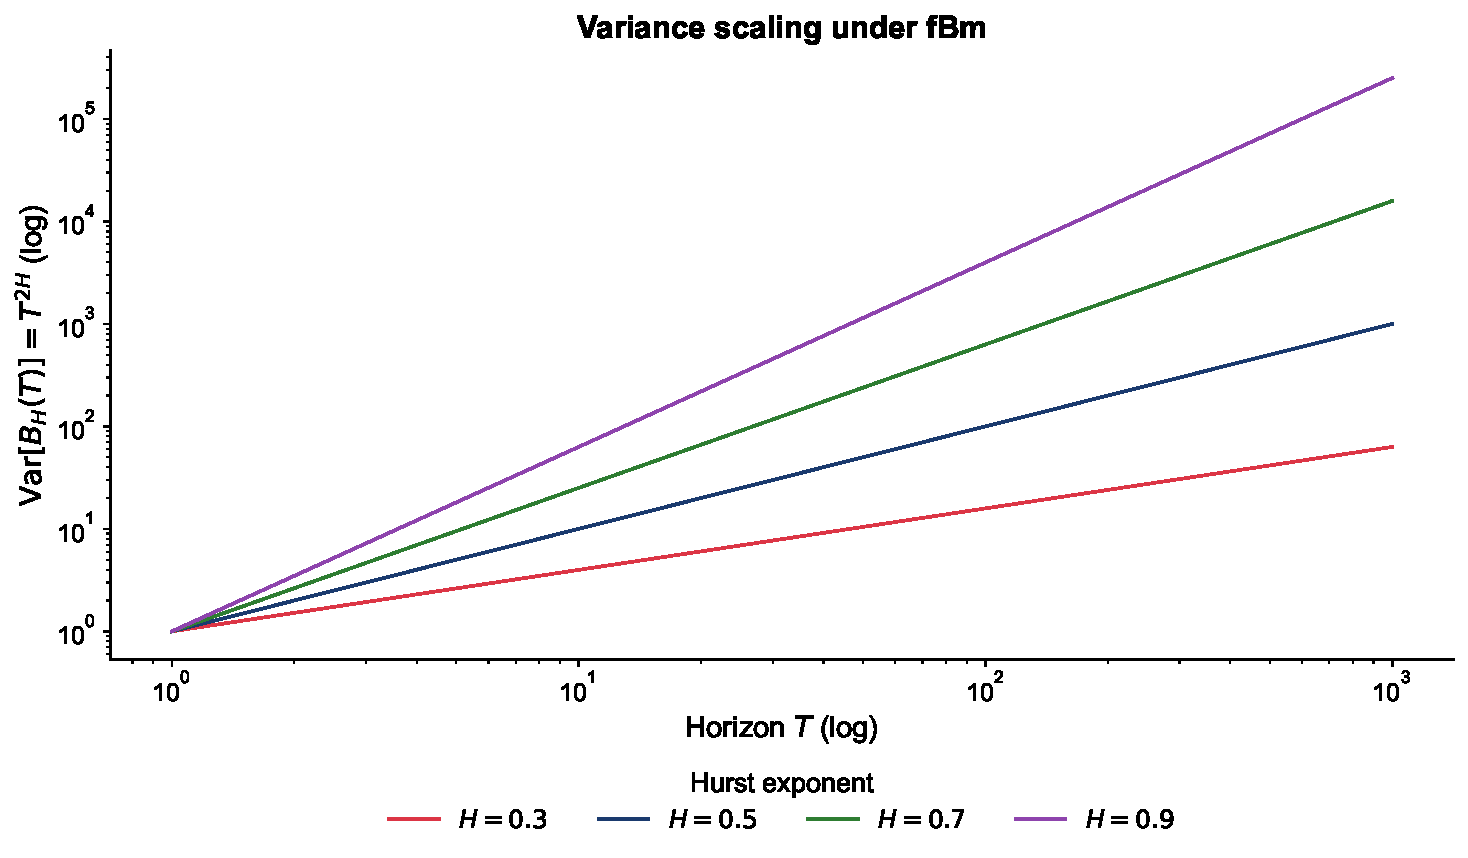
\includegraphics[width=\linewidth]{ch_fmh_var_scale_T2H.pdf}\\[0.2em]
\quantlet{SFM\_ch\_fmh\_extra}{https://github.com/QuantLet/Stat_fin_markets/tree/master/Quantlets/SFM_ch_fmh/SFM_ch_fmh_extra}
\end{column}
\begin{column}{0.37\textwidth}
\begin{block}{Cerințe}
\begin{itemize}\setlength{\itemsep}{0pt}
    \item Citiți pe grafic raportul $\text{VaR}_{T^H}/\text{VaR}_{\sqrt T}$ la $T = 10$ pentru $H = 0{,}65$
    \item Pentru $H < 0{,}5$, $\sqrt T$ supra- sau subestimează?
    \item Pentru $H > 0{,}5$ și $T$ mare, eroarea crește sau se stabilizează?
    \item Concluzionați: pentru un risc managerial de portofoliu cu $\hat H = 0{,}6$, ce sub-stres recomandați?
\end{itemize}
\end{block}
\end{column}
\end{columns}
\end{cminipage}
\end{frame}

\begin{frame}[shrink=25]{Exercițiul F8: Rezolvare}
\begin{cminipage}{0.95\textwidth}
\begin{exampleblock}{Rezolvare}
\begin{itemize}\setlength{\itemsep}{0pt}
    \item \textbf{Raport la $T = 10$, $H = 0{,}65$:}
    \begin{itemize}\setlength{\itemsep}{0pt}
        \item $T^H/\sqrt T = T^{H - 0{,}5} = 10^{0{,}15} \approx 1{,}41$
        \item $\sqrt T$ subestimează cu $\sim 41\%$
    \end{itemize}
    \item \textbf{$H < 0{,}5$:} $T^{H-0{,}5} < 1$ $\Rightarrow$ $\sqrt T$ \emph{supraestimează} (peste-rezervare)
    \item \textbf{$H > 0{,}5$, $T$ mare:} eroarea \emph{crește} cu $T$ (efect cumulativ al persistenței); divergență polynomială
    \item \textbf{Recomandare practică ($\hat H = 0{,}6$):}
    \begin{itemize}\setlength{\itemsep}{0pt}
        \item Stress-test cu $T^H$ pentru orizonturi $T \ge 5$ zile
        \item Raportare standard cu $\sqrt T$ (Basel III/FRTB)
        \item Buffer suplimentar de capital pentru senzitivitate la $H$
    \end{itemize}
\end{itemize}
\end{exampleblock}
\end{cminipage}
\end{frame}

\begin{frame}[shrink=25]{Exercițiul F9: EMH vs FMH --- comparație vizuală}
\begin{cminipage}{0.95\textwidth}
\begin{columns}[T]
\begin{column}{0.6\textwidth}
\centering
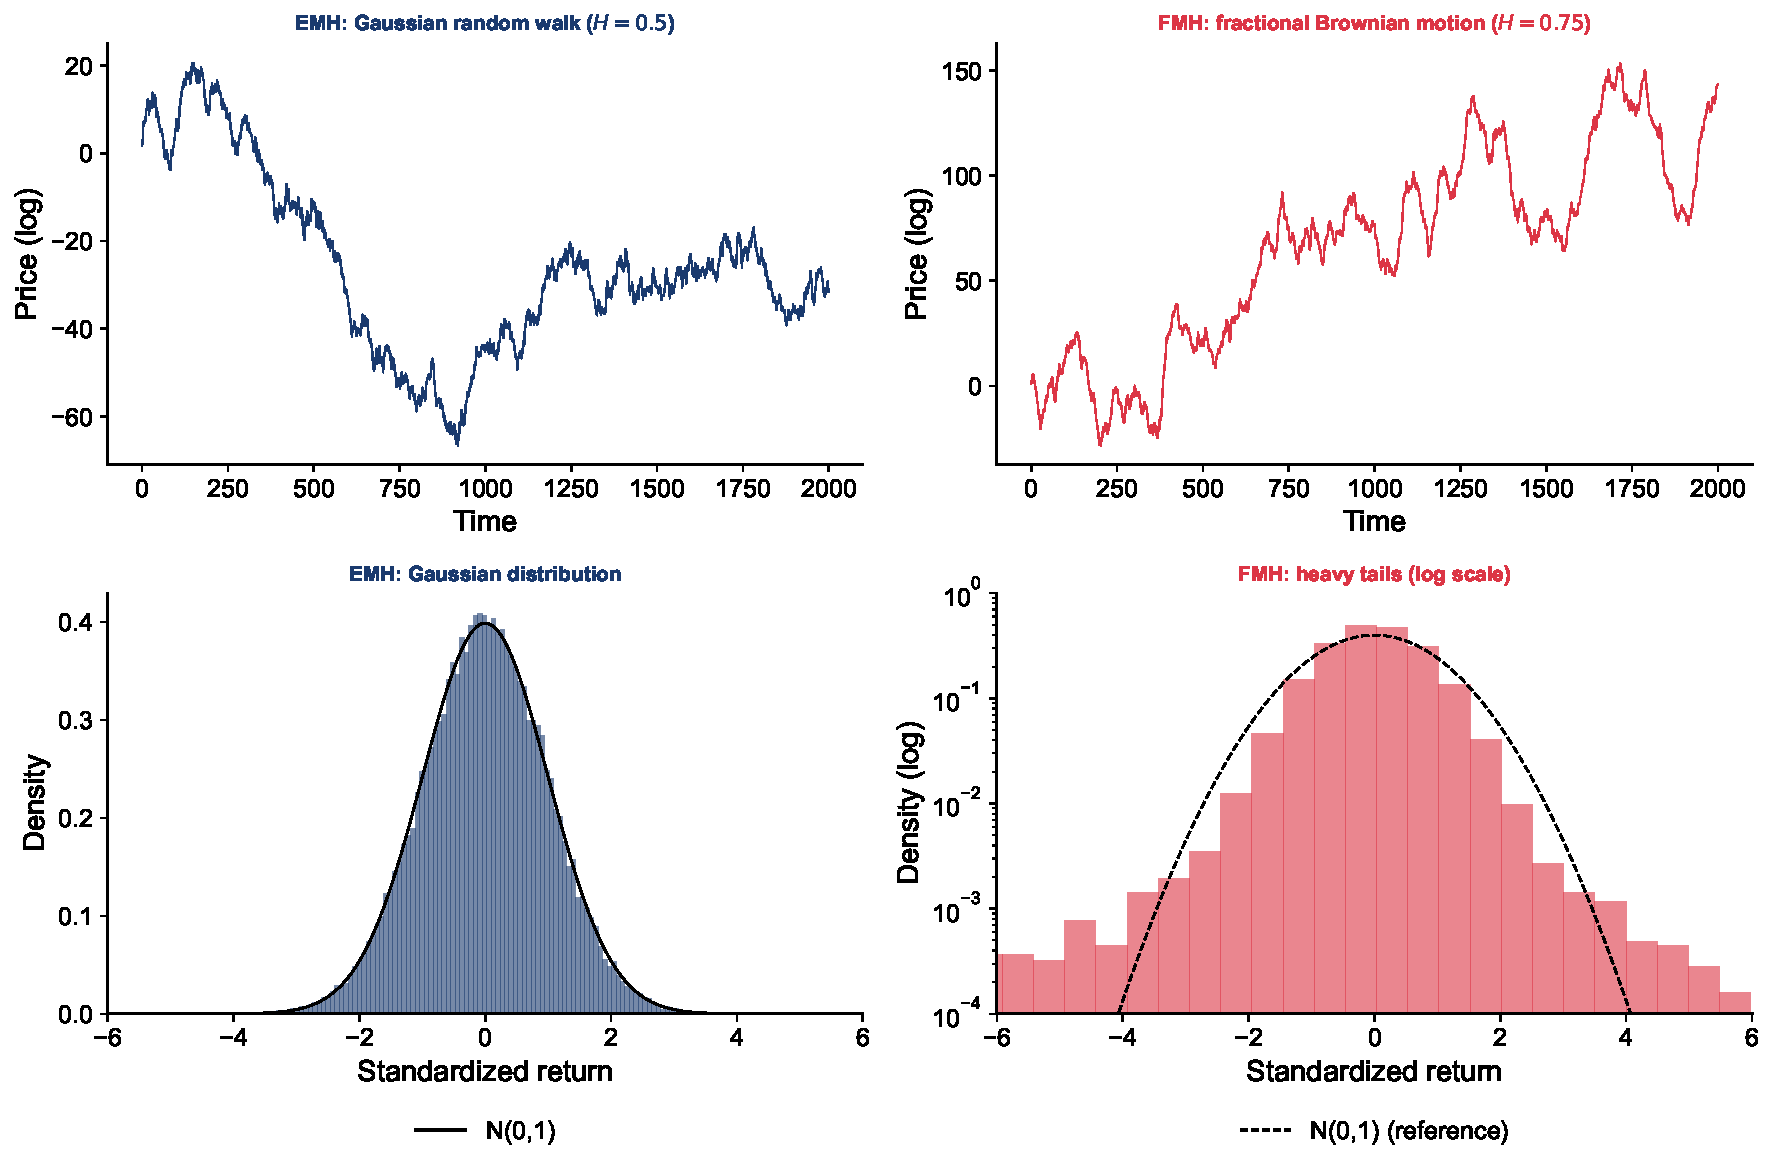
\includegraphics[width=\linewidth]{ch_fmh_emh_vs_fmh.pdf}\\[0.2em]
\quantlet{SFM\_ch\_fmh\_extra}{https://github.com/QuantLet/Stat_fin_markets/tree/master/Quantlets/SFM_ch_fmh/SFM_ch_fmh_extra}
\end{column}
\begin{column}{0.37\textwidth}
\begin{block}{Cerințe}
\begin{itemize}\setlength{\itemsep}{0pt}
    \item Identificați cele două traiectorii și ce ipoteză reprezintă fiecare
    \item Care ipoteză reflectă mai bine perioadele de criză?
    \item Cum se vede pilonul 3 Peters (colapsul orizonturilor) într-un episod de criză?
    \item Ce indicator empiric ar surprinde tranziția EMH $\to$ FMH în date reale?
\end{itemize}
\end{block}
\end{column}
\end{columns}
\end{cminipage}
\end{frame}

\begin{frame}[shrink=25]{Exercițiul F9: Rezolvare}
\begin{cminipage}{0.95\textwidth}
\begin{exampleblock}{Rezolvare}
\begin{itemize}\setlength{\itemsep}{0pt}
    \item \textbf{Traiectoria mai netedă, ``stabilă fractal''} = FMH (orizonturi diverse, lichiditate)
    \item \textbf{Traiectoria cu salturi/jumps mari, regimuri abrupte} = EMH cu fragilitate (criză)
    \item \textbf{Pilonul 3 vizibil în criză:} amplitudine bruscă, gap-uri de preț, reducerea diversității volatilității; piața trece dintr-un regim ``stabil fractal'' într-unul de panică unifrecvențială
    \item \textbf{Indicator empiric pentru tranziție:}
    \begin{itemize}\setlength{\itemsep}{0pt}
        \item $\hat H_t$ rolling (scădere bruscă $\to < 0{,}5$ în criză)
        \item Spectrul $f(\alpha)$ (lățime mai mică $\to$ mai puțin multifractală)
        \item Volatilitate realizată cu memorie scurtă (rough vol în vârf)
    \end{itemize}
\end{itemize}
\end{exampleblock}
\end{cminipage}
\end{frame}

%=============================================================================
% SUBIECT INTEGRAT
%=============================================================================
\section{Subiect integrat}

\begin{frame}[shrink=25]{Exercițiul 13 (integrat): Analiză completă Bitcoin}
\begin{cminipage}{0.95\textwidth}
\begin{block}{Enunț}
\begin{itemize}\setlength{\itemsep}{0pt}
    \item Date de piață pe $n = 1.000$ randamente zilnice Bitcoin:
    \begin{itemize}\setlength{\itemsep}{0pt}
        \item $\hat\mu_{\text{an}} = 45\%$; $\hat\sigma_{\text{an}} = 85\%$; $R_f = 3\%$
        \item Asimetrie $S = -0{,}9$; kurtosis $K = 11{,}2$; MDD $= -82\%$
    \end{itemize}
    \item Teste și estimări:
    \begin{itemize}\setlength{\itemsep}{0pt}
        \item $\hat H$ (R/S) $= 0{,}61$; $\hat\alpha$ stabilă $= 1{,}62$; $\hat\beta = -0{,}12$
        \item $Q(10) = 14{,}5$; $VR(5) = 1{,}12$; $\chi^2_{10}(0{,}05) = 18{,}31$
    \end{itemize}
    \item \textbf{Cerințe:}
    \begin{itemize}\setlength{\itemsep}{0pt}
        \item Calculați Sharpe și interpretați limitele sale
        \item Este normalitatea respinsă? Ce distribuție recomandați?
        \item Piața pare eficientă forma slabă?
        \item Recomandare finală de investiție, ținând cont de toți indicatorii
    \end{itemize}
\end{itemize}
\end{block}
\end{cminipage}
\end{frame}

\begin{frame}[shrink=25]{Exercițiul 13: Rezolvare}
\begin{cminipage}{0.95\textwidth}
\begin{exampleblock}{Rezolvare}
\small
\begin{itemize}\setlength{\itemsep}{0pt}
    \item \textbf{1. Sharpe și limite} \quad $\text{SR} = (\hat\mu - R_f)/\hat\sigma$
    \begin{itemize}\setlength{\itemsep}{0pt}
        \item $\text{SR} = (0{,}45 - 0{,}03)/0{,}85 = \mathbf{0{,}494}$
        \item Aparent decent, dar ignoră $S, K$ și MDD
        \item Sharpe singur înșelător pentru active cu cozi asimetrice
    \end{itemize}
    \item \textbf{2. Normalitate} \quad $JB = \dfrac{n}{6}\left(S^2 + \dfrac{(K-3)^2}{4}\right)$
    \begin{itemize}\setlength{\itemsep}{0pt}
        \item $JB = \frac{1000}{6}(0{,}81 + 67{,}24/4) \approx 2.937 \gg 5{,}99$
        \item Respingere covârșitoare; $\alpha = 1{,}62$ confirmă varianță infinită
        \item Recomandare: stabilă sau Student-$t$ cu $\nu \approx 4$--$5$
    \end{itemize}
    \item \textbf{3. Eficiență slabă} \quad $Q(m) \xrightarrow{H_0} \chi^2_m$;\ $VR(q) \sim q^{2H-1}$
    \begin{itemize}\setlength{\itemsep}{0pt}
        \item $Q(10) = 14{,}5 < 18{,}31 \Rightarrow$ nu respingem necorelarea
        \item Dar $VR(5) = 1{,}12 > 1$ și $H = 0{,}61 > 0{,}5$: semnale de persistență
        \item Concluzie: evidență mixtă, apropiată de eficiență slabă, compatibil cu AMH
    \end{itemize}
    \item \textbf{4. Recomandare finală:}
    \begin{itemize}\setlength{\itemsep}{0pt}
        \item MDD $-82\%$, $S = -0{,}9$, $\kappa = 8{,}2$, $\alpha = 1{,}62$, $\beta < 0$
        \item Profil extrem de riscant $\Rightarrow$ poziție mică într-un portofoliu diversificat
        \item Obligatoriu: stop-loss și conștientizarea riscului de coadă
    \end{itemize}
\end{itemize}
\end{exampleblock}
\end{cminipage}
\end{frame}

%=============================================================================
% INTERPRETARE OUTPUT-URI
%=============================================================================
\section{Interpretare: tabele, grafice, output-uri Python}

\begin{frame}[shrink=25]{Exercițiul 14: Tabel statistici descriptive multi-activ}
\begin{cminipage}{0.95\textwidth}
\begin{block}{Enunț --- output descriptive.py}
\small
\renewcommand{\arraystretch}{1.2}
\begin{center}
\begin{tabular}{lrrrrrr}
\toprule
\textbf{Activ} & $\hat\mu_{\text{zi}}$ (\%) & $\hat\sigma_{\text{zi}}$ (\%) & $S$ & $K$ & $JB$ & $p$-$JB$ \\
\midrule
S\&P~500 & $0{,}035$ & $1{,}10$ & $-0{,}45$ & $8{,}2$ & $1.158$ & $< 0{,}001$ \\
Gold (XAU) & $0{,}028$ & $0{,}95$ & $-0{,}12$ & $5{,}4$ & $261$ & $< 0{,}001$ \\
Bitcoin & $0{,}080$ & $4{,}20$ & $-0{,}95$ & $14{,}8$ & $5.994$ & $< 0{,}001$ \\
\bottomrule
\end{tabular}
\end{center}
Eșantion: $n = 1.000$ zile per activ, $\chi^2_2(0{,}05) = 5{,}99$.
\end{block}
\begin{itemize}\setlength{\itemsep}{0pt}
    \item \textbf{Cerințe:}
    \begin{itemize}\setlength{\itemsep}{0pt}
        \item Se respinge normalitatea pentru toate cele 3 active?
        \item Care activ are cozile cele mai grele? Care are asimetrie cea mai negativă?
        \item Clasați activele după raport randament/risc brut ($\hat\mu / \hat\sigma$)
        \item Recomandați o distribuție adecvată pentru fiecare
    \end{itemize}
\end{itemize}
\end{cminipage}
\end{frame}

\begin{frame}[shrink=25]{Exercițiul 14: Rezolvare}
\begin{cminipage}{0.95\textwidth}
\begin{exampleblock}{Rezolvare}
\begin{itemize}\setlength{\itemsep}{0pt}
    \item \textbf{1. Normalitate} \quad respingem $H_0$ dacă $JB > \chi^2_2(0{,}05) = 5{,}99$
    \begin{itemize}\setlength{\itemsep}{0pt}
        \item Toate $JB \gg 5{,}99$, toate $p < 0{,}001$ $\Rightarrow$ respingere unanimă
        \item \textit{Interpretare:} normalitatea respinsă \emph{universal} pe orice activ financiar real cu $n \ge 1.000$. ``Randamentele sunt log-normale'' este idealizare didactică, nu realitate
    \end{itemize}
    \item \textbf{2. Cozi și asimetrie:}
    \begin{itemize}\setlength{\itemsep}{0pt}
        \item Bitcoin: $K = 14{,}8$ (cele mai groase cozi);\ $S = -0{,}95$
        \item Gold: $S = -0{,}12$, aproape simetric
        \item \textit{Interpretare:} BTC combină cozi grele \emph{și} asimetrie negativă $\Rightarrow$ tail-risk extrem; Gold este \emph{flight to quality}
    \end{itemize}
    \item \textbf{3. Randament/risc brut (proxy Sharpe $\hat\mu/\hat\sigma$):}
    \begin{itemize}\setlength{\itemsep}{0pt}
        \item S\&P~500: $0{,}0318$;\ Gold: $0{,}0295$;\ Bitcoin: $0{,}0190$ (ultimul!)
        \item \textit{Interpretare:} BTC pierde clasamentul în ciuda lui $\mu$ mare; $\sigma$ e disproporționat. Randamentul absolut e înșelător --- doar raportul cu riscul contează
    \end{itemize}
    \item \textbf{4. Distribuții recomandate:}
    \begin{itemize}\setlength{\itemsep}{0pt}
        \item Gold: Student-$t$ cu $\nu = 4 + 6/2{,}4 \approx 6{,}5$
        \item S\&P~500: Student-$t$ cu $\nu \approx 5$ sau stabilă $\alpha \approx 1{,}8$
        \item Bitcoin: stabilă $\alpha < 1{,}7$, $\beta < 0$ sau Student-$t$ cu $\nu \approx 4$
        \item \textit{Interpretare:} pentru risc management ales conservativ (coadă mai grea); pentru fitting estetic AIC/BIC selectează parsimonios
    \end{itemize}
\end{itemize}
\end{exampleblock}
\end{cminipage}
\end{frame}

\begin{frame}[fragile, shrink=25]{Exercițiul 15: Output Python --- teste de eficiență}
\begin{cminipage}{0.95\textwidth}
\begin{block}{Enunț --- output Python pe randamente BET (BVB), $n = 1.200$}
\begin{lstlisting}[basicstyle=\ttfamily\scriptsize, frame=single]
>>> from statsmodels.stats.diagnostic import acorr_ljungbox
>>> acorr_ljungbox(returns, lags=[5, 10, 20])
      lb_stat   lb_pvalue
5     18.34     0.0026
10    24.87     0.0056
20    38.12     0.0086

>>> variance_ratio(returns, q=[2, 5, 10])
  q    VR      Z       p-value
  2    1.18    2.89    0.0039
  5    1.32    3.14    0.0017
  10   1.41    3.05    0.0023

>>> runs_test(np.sign(returns))
  R = 612, E[R] = 598, Z = 0.89, p = 0.374
\end{lstlisting}
\end{block}
\begin{itemize}\setlength{\itemsep}{0pt}
    \item \textbf{Cerințe:}
    \begin{itemize}\setlength{\itemsep}{0pt}
        \item Interpretați fiecare test la $\alpha = 5\%$
        \item De ce testul runs nu respinge $H_0$, dar Ljung--Box și VR da?
        \item Ce direcție indică $VR > 1$? Compatibil cu EMH slabă?
        \item Posibile cauze ale autocorelației pe BVB
    \end{itemize}
\end{itemize}
\end{cminipage}
\end{frame}

\begin{frame}[shrink=25]{Exercițiul 15: Rezolvare}
\begin{cminipage}{0.95\textwidth}
\begin{exampleblock}{Rezolvare}
\begin{itemize}\setlength{\itemsep}{0pt}
    \item \textbf{1. Interpretare pe test:}
    \begin{itemize}\setlength{\itemsep}{0pt}
        \item Ljung--Box: toate $p < 0{,}05$ $\Rightarrow$ respingem $H_0$ la toate lag-urile
        \item Variance ratio: toate $p < 0{,}05$ $\Rightarrow$ respingem RW pe toate orizonturile
        \item Runs test: $p = 0{,}374 > 0{,}05$ $\Rightarrow$ semnele par independente
        \item \textit{Interpretare:} discrepanță elocventă --- LB și VR (folosesc valorile) detectează structură; runs (doar semnele) nu. Dependența e \emph{în magnitudine}, nu în semn
    \end{itemize}
    \item \textbf{2. De ce runs ok dar LB/VR resping:}
    \begin{itemize}\setlength{\itemsep}{0pt}
        \item Runs folosește \textbf{doar semnele}; LB/VR folosesc valorile cu magnitudine
        \item \textit{Interpretare:} runs are putere statistică redusă pentru $\hat\rho$ mic-pozitiv; adecvat doar pentru detecții brute (clustering de semne). \emph{Nu folosiți runs ca singur diagnostic} pentru EMH
    \end{itemize}
    \item \textbf{3. Direcția $VR > 1$:}
    \begin{itemize}\setlength{\itemsep}{0pt}
        \item $VR(2) = 1{,}18 \to VR(10) = 1{,}41 > 1$ $\Rightarrow$ \textbf{momentum}
        \item \textit{Interpretare:} $VR$ crește cu $q$ $\Rightarrow$ memorie persistentă. Hurst echivalent: $\hat H \approx 0{,}57$. \textbf{Incompatibil} cu EMH slabă strictă
    \end{itemize}
    \item \textbf{4. Cauze probabile pe BVB:}
    \begin{itemize}\setlength{\itemsep}{0pt}
        \item Thin trading (non-sincronizarea tranzacțiilor între acțiuni)
        \item Lichiditate redusă $\Rightarrow$ ajustare lentă la informație
        \item Număr mic de participanți sofisticați $\Rightarrow$ ineficiență reziduală
        \item \textit{Interpretare:} BVB e piață frontier/emergentă; ineficiențe sunt așteptate. Dar costurile de tranzacție ($\sim 0{,}65\%$ round-trip) depășesc adesea $\hat\rho$ exploatabil $\Rightarrow$ ineficiență statistică \emph{nu} traducere automat în profit
    \end{itemize}
\end{itemize}
\end{exampleblock}
\end{cminipage}
\end{frame}

\begin{frame}[shrink=30]{Exercițiul 16: Grafic QQ-plot --- identificați distribuția}
\begin{cminipage}{0.95\textwidth}
\begin{columns}[T]
\begin{column}{0.55\textwidth}
\centering
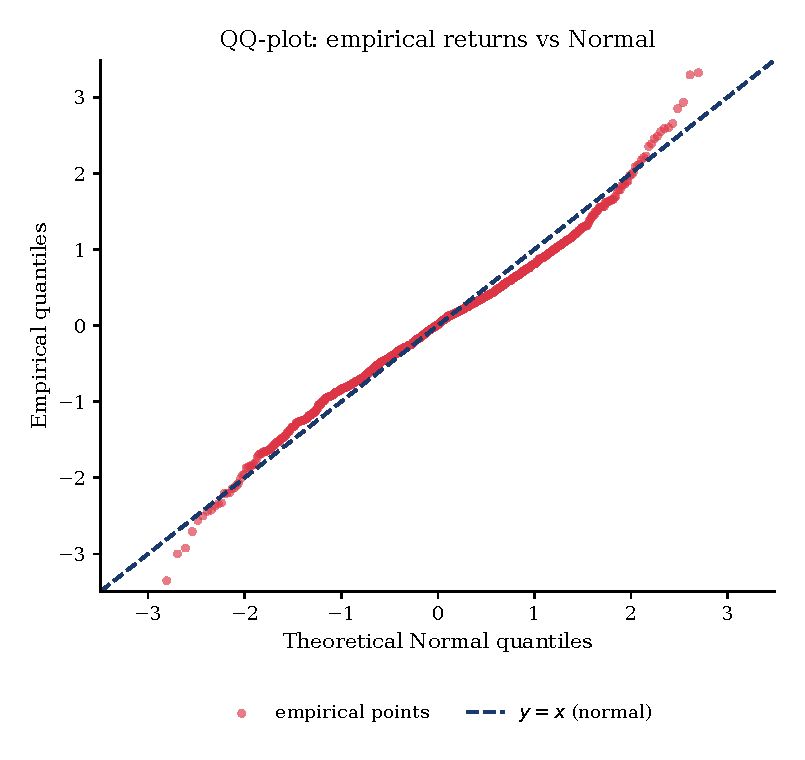
\includegraphics[width=0.78\linewidth]{sfm_sem_recap_qq.pdf}
\end{column}
\begin{column}{0.42\textwidth}
\begin{itemize}\setlength{\itemsep}{0pt}
    \item \textbf{Cerințe:}
    \begin{itemize}\setlength{\itemsep}{0pt}
        \item Descrieți pattern-ul QQ; unde deviază de la $y = x$?
        \item Ce semnifică abaterile la extremități și zona centrală?
        \item Ce distribuție alternativă ar produce un QQ aproape liniar?
    \end{itemize}
\end{itemize}
\end{column}
\end{columns}
\end{cminipage}
\quantlet{SFM\_sem\_recap\_plots}{https://colab.research.google.com/github/QuantLet/Stat_fin_markets/blob/master/Sem_recap/SFM_sem_recap_plots/SFM_sem_recap_plots.ipynb}
\end{frame}

\begin{frame}[shrink=25]{Exercițiul 16: Rezolvare}
\begin{cminipage}{0.95\textwidth}
\begin{exampleblock}{Rezolvare}
\begin{itemize}\setlength{\itemsep}{0pt}
    \item \textbf{1. Pattern-ul QQ:}
    \begin{itemize}\setlength{\itemsep}{0pt}
        \item În zona centrală: puncte aproape de $y = x$ (distribuție normală la centru)
        \item La stânga: puncte $\mathbf{sub}$ linia $y = x$ (cuantile empirice $< $ teoretice)
        \item La dreapta: puncte \textbf{deasupra} liniei $y = x$ (cuantile empirice $>$ teoretice)
    \end{itemize}
    \item \textbf{2. Abateri la extremități:}
    \begin{itemize}\setlength{\itemsep}{0pt}
        \item Forma ``S'' inversată $\Rightarrow$ cozi mai groase decât normala
        \item Pierderi extreme mai mari decât prezice modelul normal
        \item Câștiguri extreme de asemenea mai mari
    \end{itemize}
    \item \textbf{3. Zona centrală aproape liniară:}
    \begin{itemize}\setlength{\itemsep}{0pt}
        \item Comportamentul ``tipic'' este aproximativ normal
        \item Abaterile se concentrează în cozi $\Rightarrow$ leptokurtic
    \end{itemize}
    \item \textbf{4. Distribuții alternative:}
    \begin{itemize}\setlength{\itemsep}{0pt}
        \item Student-$t$ cu $\nu \in [4, 6]$ --- centrul aproape normal, cozi mai groase
        \item Stabilă cu $\alpha \in [1{,}6, 1{,}9]$ --- cozi polinomiale
        \item Nu recomandăm Cauchy ($\alpha = 1$): abaterile observate sunt moderate, nu extreme
    \end{itemize}
\end{itemize}
\end{exampleblock}
\end{cminipage}
\end{frame}

\begin{frame}[shrink=25]{Exercițiul 17: Event study --- tabel CAR multi-fereastră}
\begin{cminipage}{0.95\textwidth}
\begin{block}{Enunț --- output event study pe $N = 80$ firme}
\small
\renewcommand{\arraystretch}{1.2}
\begin{center}
\begin{tabular}{lrrrl}
\toprule
\textbf{Fereastră} & \textbf{CAR mediu (\%)} & \textbf{$t$-stat} & \textbf{$p$-value} & \textbf{Semnificativ?} \\
\midrule
$[-10, -2]$ (pre-eveniment) & $+0{,}81$ & $1{,}42$ & $0{,}156$ & Nu \\
$[-1, +1]$ (eveniment) & $+2{,}95$ & $5{,}12$ & $< 0{,}001$ & \textbf{Da} \\
$[+2, +5]$ (post-1) & $+0{,}74$ & $2{,}18$ & $0{,}029$ & \textbf{Da} \\
$[+6, +20]$ (post-2) & $+1{,}32$ & $3{,}45$ & $< 0{,}001$ & \textbf{Da} \\
\bottomrule
\end{tabular}
\end{center}
Valori critice: $t_{0{,}025, \infty} = 1{,}96$; $t_{0{,}005, \infty} = 2{,}58$.
\end{block}
\begin{itemize}\setlength{\itemsep}{0pt}
    \item \textbf{Cerințe:}
    \begin{itemize}\setlength{\itemsep}{0pt}
        \item A existat scurgere de informație pre-eveniment?
        \item Piața a reacționat complet la anunț în fereastra $[-1, +1]$?
        \item Ce anomalie este evidențiată de ferestrele post-eveniment?
        \item Este compatibil cu EMH semi-tare? Argumentați
    \end{itemize}
\end{itemize}
\end{cminipage}
\end{frame}

\begin{frame}[shrink=25]{Exercițiul 17: Rezolvare}
\begin{cminipage}{0.95\textwidth}
\begin{exampleblock}{Rezolvare}
\begin{itemize}\setlength{\itemsep}{0pt}
    \item \textbf{1. Scurgere pre-eveniment:}
    \begin{itemize}\setlength{\itemsep}{0pt}
        \item CAR$[-10, -2] = +0{,}81\%$, $p = 0{,}156 > 0{,}05$ $\Rightarrow$ nesemnificativ
        \item \textbf{Nu există dovadă de scurgere} de informație în cele 8 zile pre-anunț
    \end{itemize}
    \item \textbf{2. Reacția în fereastra de eveniment:}
    \begin{itemize}\setlength{\itemsep}{0pt}
        \item CAR$[-1, +1] = +2{,}95\%$, $t = 5{,}12$, $p < 0{,}001$: reacție puternică și rapidă
        \item Dar CAR$[+2, +5] = +0{,}74\%$, $p = 0{,}029$: \textbf{drift pozitiv persistent}
        \item Deci reacția \textbf{nu este completă} în $[-1, +1]$
    \end{itemize}
    \item \textbf{3. Anomalia din ferestrele post-eveniment:}
    \begin{itemize}\setlength{\itemsep}{0pt}
        \item CAR$[+6, +20] = +1{,}32\%$, $p < 0{,}001$: drift pozitiv continuă 4 săptămâni
        \item Fenomen: \textbf{Post-Earnings Announcement Drift (PEAD)}
        \item Piața încorporează informația treptat, nu instantaneu
    \end{itemize}
    \item \textbf{4. EMH semi-tare:}
    \begin{itemize}\setlength{\itemsep}{0pt}
        \item \textbf{Incompatibil} cu EMH semi-tare: PEAD = drift predictibil după informație publică
        \item Anomalia PEAD este bine documentată (Bernard \& Thomas, 1989)
        \item Evidență pentru ineficiență locală, exploatabilă înainte de costuri
    \end{itemize}
\end{itemize}
\end{exampleblock}
\end{cminipage}
\end{frame}

%=============================================================================
% EXERCIȚII SUPLIMENTARE GRAFICE + TABELE
%=============================================================================

\begin{frame}[shrink=30]{Exercițiul 18: Autocorelograma --- grafic ACF}
\begin{cminipage}{0.95\textwidth}
\begin{columns}[T]
\begin{column}{0.6\textwidth}
\begin{block}{Enunț --- ACF randamente zilnice, $n = 500$}
\centering
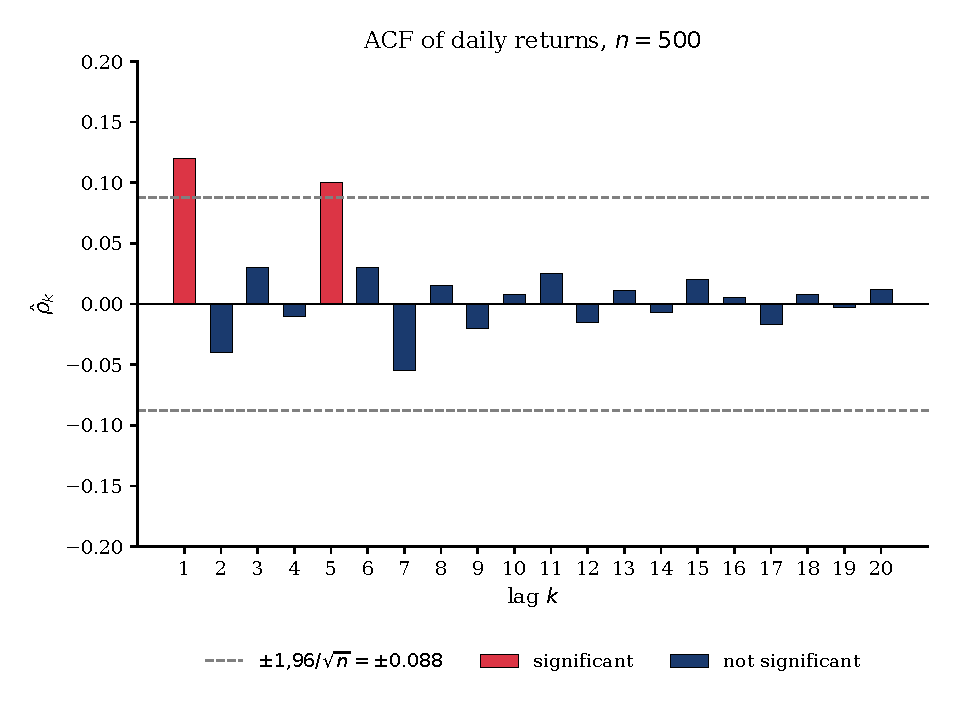
\includegraphics[width=0.85\linewidth]{sfm_sem_recap_acf.pdf}
\end{block}
\end{column}
\begin{column}{0.37\textwidth}
\begin{itemize}\setlength{\itemsep}{0pt}
    \item \textbf{Cerințe:}
    \begin{itemize}\setlength{\itemsep}{0pt}
        \item Care lag-uri depășesc banda $\pm 1{,}96/\sqrt{n}$?
        \item $\pm 1{,}96/\sqrt{500} \approx \pm 0{,}088$
        \item Autocorelații izolate sau periodice?
        \item Este piața compatibilă cu EMH slabă?
        \item Ce efect posibil explică lag-ul 5?
    \end{itemize}
\end{itemize}
\end{column}
\end{columns}
\end{cminipage}
\vspace{0.05cm}
\quantlet{SFM\_sem\_recap\_plots}{https://colab.research.google.com/github/QuantLet/Stat_fin_markets/blob/master/Sem_recap/SFM_sem_recap_plots/SFM_sem_recap_plots.ipynb}
\end{frame}

\begin{frame}[shrink=25]{Exercițiul 18: Rezolvare}
\begin{cminipage}{0.95\textwidth}
\begin{exampleblock}{Rezolvare}
\begin{itemize}\setlength{\itemsep}{0pt}
    \item \textbf{1. Lag-uri semnificative:}
    \begin{itemize}\setlength{\itemsep}{0pt}
        \item Banda de încredere: $\pm 0{,}088$
        \item Lag 1: $\hat\rho_1 = 0{,}12 > 0{,}088$ --- \textcolor{Crimson}{semnificativ}
        \item Lag 5: $\hat\rho_5 = 0{,}10 > 0{,}088$ --- \textcolor{Crimson}{semnificativ}
        \item Lag 7: $\hat\rho_7 \approx -0{,}055$ --- sub bandă (nesemnificativ)
        \item Toate celelalte: în interiorul benzii
    \end{itemize}
    \item \textbf{2. Pattern observat:}
    \begin{itemize}\setlength{\itemsep}{0pt}
        \item Autocorelații izolate (doar lag 1 și 5), nu descreștere exponențială
        \item Nu este un pattern AR(1) clasic
    \end{itemize}
    \item \textbf{3. EMH slabă:}
    \begin{itemize}\setlength{\itemsep}{0pt}
        \item Două lag-uri semnificative $\Rightarrow$ respingem ipoteza de necorelare totală
        \item \textbf{Ușoară ineficiență}, dar magnitudine mică ($\hat\rho < 0{,}15$)
        \item În practică: greu exploatabilă după costuri de tranzacție
    \end{itemize}
    \item \textbf{4. Posibile cauze pentru lag 5:}
    \begin{itemize}\setlength{\itemsep}{0pt}
        \item Efect săptămânal (week-end effect): luni diferă de vineri
        \item Reechilibrare săptămânală a fondurilor mari
        \item Thin trading sau anunțuri macro cu frecvență săptămânală
    \end{itemize}
\end{itemize}
\end{exampleblock}
\end{cminipage}
\end{frame}

\begin{frame}[shrink=30]{Exercițiul 19: Rolling volatility --- identificați regimurile}
\begin{cminipage}{0.95\textwidth}
\begin{columns}[T]
\begin{column}{0.6\textwidth}
\begin{block}{Enunț --- $\hat\sigma$ rolling (3M), 2018--2024}
\centering
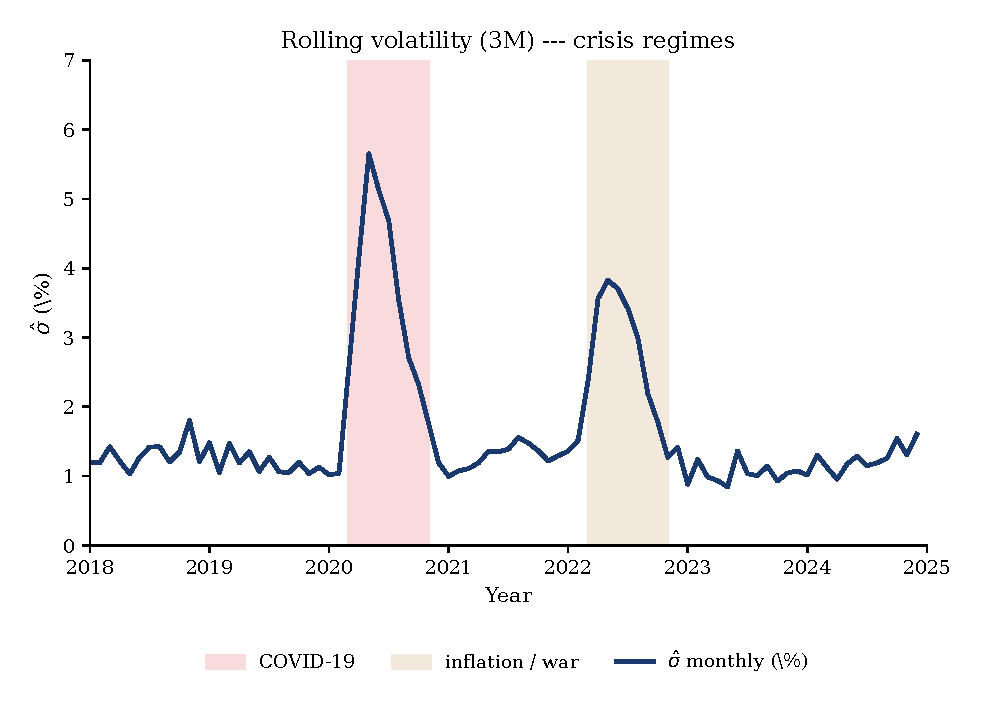
\includegraphics[width=0.85\linewidth]{sfm_sem_recap_volregimes.pdf}
\end{block}
\end{column}
\begin{column}{0.37\textwidth}
\begin{itemize}\setlength{\itemsep}{0pt}
    \item \textbf{Cerințe:}
    \begin{itemize}\setlength{\itemsep}{0pt}
        \item Identificați 2 regimuri de volatilitate
        \item Care este ``fapta stilizată''?
        \item Raportul criză / bazal
        \item Implicații pentru modelarea riscului
        \item Ce model statistic captează fenomenul?
    \end{itemize}
\end{itemize}
\end{column}
\end{columns}
\end{cminipage}
\vspace{0.05cm}
\quantlet{SFM\_sem\_recap\_plots}{https://colab.research.google.com/github/QuantLet/Stat_fin_markets/blob/master/Sem_recap/SFM_sem_recap_plots/SFM_sem_recap_plots.ipynb}
\end{frame}

\begin{frame}[shrink=25]{Exercițiul 19: Rezolvare}
\begin{cminipage}{0.95\textwidth}
\begin{exampleblock}{Rezolvare}
\begin{itemize}\setlength{\itemsep}{0pt}
    \item \textbf{1. Regimuri identificate:}
    \begin{itemize}\setlength{\itemsep}{0pt}
        \item Regim ``calm'': $\hat\sigma \approx 1$--$1{,}5\%$ (2018--2019, 2021, 2023--2024)
        \item Regim ``criză'': $\hat\sigma \approx 3$--$6\%$ (martie 2020 COVID, 2022 inflație/război)
    \end{itemize}
    \item \textbf{2. Fapta stilizată demonstrată:}
    \begin{itemize}\setlength{\itemsep}{0pt}
        \item \textbf{Clustering de volatilitate} (Mandelbrot, 1963)
        \item Zile cu volatilitate mare urmate de zile cu volatilitate mare
    \end{itemize}
    \item \textbf{3. Raport bazal vs criză:}
    \begin{itemize}\setlength{\itemsep}{0pt}
        \item COVID: $5{,}8/1{,}3 \approx 4{,}5\times$ volatilitatea bazală
        \item 2022: $3{,}8/1{,}4 \approx 2{,}7\times$
    \end{itemize}
    \item \textbf{4. Implicații pentru modelarea riscului:}
    \begin{itemize}\setlength{\itemsep}{0pt}
        \item Ipoteza $\sigma$ constantă este \textbf{grav încălcată}
        \item Regula $\sqrt{T}$ subestimează riscul în perioade de criză
        \item Estimatorul rolling sau realizat este necesar
    \end{itemize}
    \item \textbf{5. Model recomandat:}
    \begin{itemize}\setlength{\itemsep}{0pt}
        \item GARCH (volatilitate condiționată autoregresivă)
        \item Stochastic volatility models (SV)
        \item Realized volatility (RV) pe date intra-zilnice
    \end{itemize}
\end{itemize}
\end{exampleblock}
\end{cminipage}
\end{frame}

\begin{frame}[shrink=30]{Exercițiul 20: Tabel + grafic --- alegerea fondului optim}
\begin{cminipage}{0.95\textwidth}
\begin{block}{Enunț --- 5 fonduri de investiții, anualizat, $R_f = 2\%$}
\begin{columns}[T]
\begin{column}{0.54\textwidth}
\scriptsize
\renewcommand{\arraystretch}{1.05}
\begin{tabular}{lrrrrrr}
\toprule
\textbf{Fond} & $\hat\mu$\% & $\hat\sigma$\% & \textbf{Sh} & \textbf{So} & \textbf{MDD}\% & \textbf{Ca} \\
\midrule
Alpha (tech) & $18$ & $28$ & $0{,}57$ & $0{,}68$ & $-42$ & $0{,}43$ \\
Beta (divers.)  & $10$ & $12$ & $0{,}67$ & $0{,}85$ & $-15$ & $0{,}67$ \\
Gamma (obl.) & $5$  & $4$  & $0{,}75$ & $1{,}10$ & $-6$  & $0{,}83$ \\
Delta (hedge)  & $14$ & $18$ & $0{,}67$ & $0{,}90$ & $-22$ & $0{,}64$ \\
Epsilon (EM)  & $22$ & $45$ & $0{,}44$ & $0{,}48$ & $-65$ & $0{,}34$ \\
\bottomrule
\end{tabular}

{\tiny Sh = Sharpe, So = Sortino, Ca = Calmar}
\end{column}
\begin{column}{0.44\textwidth}
\centering
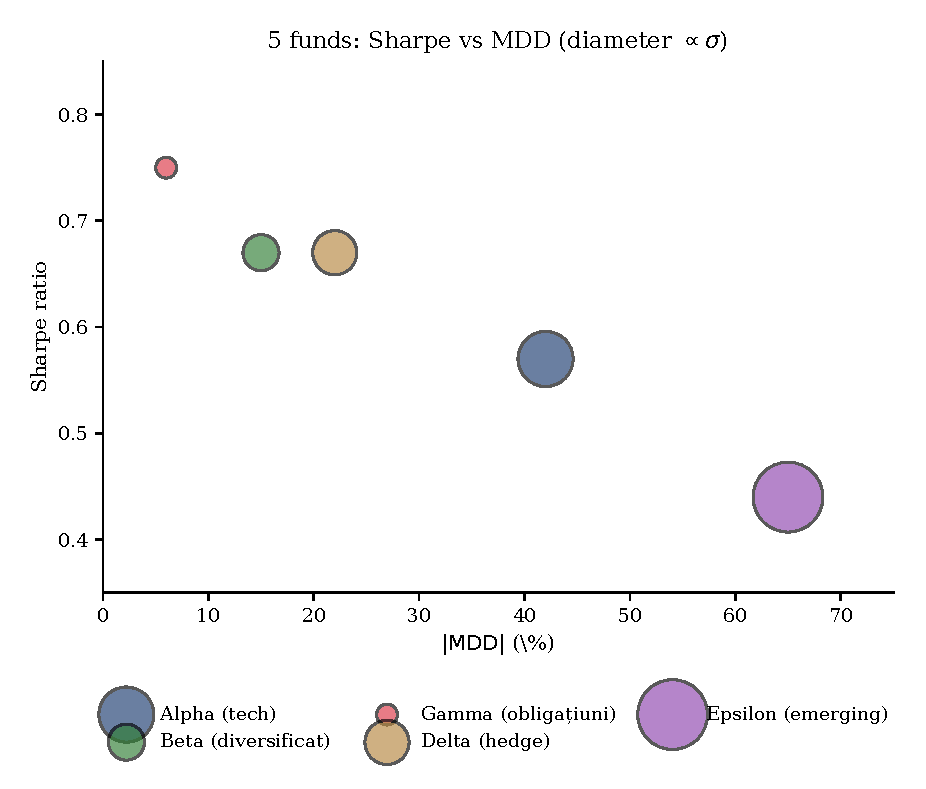
\includegraphics[width=0.85\linewidth]{sfm_sem_recap_funds_bubble.pdf}
\end{column}
\end{columns}
\end{block}
\begin{itemize}\setlength{\itemsep}{0pt}
    \item \textbf{Cerințe:}
    \begin{itemize}\setlength{\itemsep}{0pt}
        \item Câștigătorul după Sharpe / Sortino / Calmar?
        \item De ce Sortino $>$ Sharpe la toate? Ce implică?
        \item Ce fond pentru investitor avers la risc vs.\ tolerant la risc?
    \end{itemize}
\end{itemize}
\end{cminipage}
\quantlet{SFM\_sem\_recap\_plots}{https://colab.research.google.com/github/QuantLet/Stat_fin_markets/blob/master/Sem_recap/SFM_sem_recap_plots/SFM_sem_recap_plots.ipynb}
\end{frame}

\begin{frame}[shrink=25]{Exercițiul 20: Rezolvare}
\begin{cminipage}{0.95\textwidth}
\begin{exampleblock}{Rezolvare}
\begin{itemize}\setlength{\itemsep}{0pt}
    \item \textbf{1. Câștigători pe fiecare criteriu:}
    \begin{itemize}\setlength{\itemsep}{0pt}
        \item Sharpe maxim: \textbf{Gamma} ($0{,}75$) --- obligațiuni, risc mic
        \item Sortino maxim: \textbf{Gamma} ($1{,}10$) --- asimetrie favorabilă
        \item Calmar maxim: \textbf{Gamma} ($0{,}83$) --- pierderea maximă mică
    \end{itemize}
    \item \textbf{2. Sortino $>$ Sharpe la toate:}
    \begin{itemize}\setlength{\itemsep}{0pt}
        \item Sortino penalizează doar varianța negativă (downside)
        \item $\sigma_{\text{downside}} < \sigma$ $\Rightarrow$ Sortino $>$ Sharpe
        \item Implică: randamentele pozitive contribuie la $\sigma$ total, dar nu ne deranjează
    \end{itemize}
    \item \textbf{3. Ce aduce Calmar:}
    \begin{itemize}\setlength{\itemsep}{0pt}
        \item Sharpe ignoră MDD --- un fond poate avea Sharpe bun dar MDD catastrofal
        \item Calmar $= \hat\mu/|\text{MDD}|$ penalizează direct pierderea maximă
        \item Important pentru investitori care nu tolerează pierderi adânci
    \end{itemize}
    \item \textbf{4. Investitor avers la risc:}
    \begin{itemize}\setlength{\itemsep}{0pt}
        \item \textbf{Gamma}: câștigă pe toate criteriile, MDD $= -6\%$ acceptabil
        \item Alternativ Beta: randament mai mare, MDD $-15\%$ moderat
    \end{itemize}
    \item \textbf{5. Investitor tolerant la risc:}
    \begin{itemize}\setlength{\itemsep}{0pt}
        \item \textbf{Epsilon}: $\hat\mu = 22\%$ dar MDD $-65\%$ (atenție la coada stângă)
        \item Alternativ Alpha sau combinație Alpha + Gamma
    \end{itemize}
\end{itemize}
\end{exampleblock}
\end{cminipage}
\end{frame}

\begin{frame}[shrink=25]{Exercițiul 21: Tabel regresie CAPM --- interpretare output}
\begin{cminipage}{0.95\textwidth}
\begin{block}{Enunț --- output regresie $r_{i,t} - R_f = \alpha + \beta(r_{m,t} - R_f) + \varepsilon_t$}
\small
\renewcommand{\arraystretch}{1.2}
\begin{center}
\begin{tabular}{lrrrr}
\toprule
\textbf{Acțiune} & $\hat\alpha$ (\%, an.) & $\hat\beta$ & $R^2$ & $t(\hat\alpha)$ \\
\midrule
Apple (AAPL) & $3{,}8$ & $1{,}18$ & $0{,}51$ & $2{,}14$ \\
Procter \& Gamble (PG) & $0{,}9$ & $0{,}54$ & $0{,}28$ & $0{,}78$ \\
JPMorgan (JPM) & $1{,}2$ & $1{,}35$ & $0{,}58$ & $0{,}91$ \\
Tesla (TSLA) & $8{,}5$ & $2{,}10$ & $0{,}33$ & $3{,}02$ \\
Johnson \& Johnson (JNJ) & $-0{,}5$ & $0{,}62$ & $0{,}31$ & $-0{,}42$ \\
\bottomrule
\end{tabular}
\end{center}
Date zilnice 2019--2024, $n = 1.260$. Valoare critică: $t_{0{,}025, \infty} = 1{,}96$.
\end{block}
\begin{itemize}\setlength{\itemsep}{0pt}
    \item \textbf{Cerințe:}
    \begin{itemize}\setlength{\itemsep}{0pt}
        \item Care acțiuni sunt \textbf{agresive} ($\beta > 1$) și care \textbf{defensive} ($\beta < 1$)?
        \item Pentru care acțiuni $\hat\alpha$ este semnificativ pozitiv la 5\%?
        \item Ce semnifică $R^2$ scăzut pentru PG? Dar $R^2$ ridicat pentru AAPL și JPM?
        \item Testul $\alpha$ semnificativ se leagă de EMH semi-tare. Cum?
        \item Ce acțiune recomandați pentru o scădere a pieței? (beta low)
    \end{itemize}
\end{itemize}
\end{cminipage}
\end{frame}

\begin{frame}[shrink=35]{Exercițiul 21: Rezolvare}
\begin{cminipage}{0.95\textwidth}
\begin{exampleblock}{Rezolvare}
\begin{itemize}\setlength{\itemsep}{0pt}
    \item \textbf{1. Clasificare după $\beta$} \quad $\beta = \Cov(r_i, r_m)/\Var(r_m)$
    \begin{itemize}\setlength{\itemsep}{0pt}
        \item Agresive ($\beta > 1$): AAPL ($1{,}18$), JPM ($1{,}35$), TSLA ($2{,}10$)
        \item Defensive ($\beta < 1$): PG ($0{,}54$), JNJ ($0{,}62$)
        \item \textit{Interpretare:} TSLA cu $\beta = 2{,}1$ se mișcă \emph{de două ori} cât piața --- amplifică câștigurile dar și pierderile. Defensive (consum staples, healthcare) preferate ca ``crisis hedge''
    \end{itemize}
    \item \textbf{2. $\hat\alpha$ semnificativ pozitiv} \quad $|t(\hat\alpha)| > 1{,}96$ la 5\%
    \begin{itemize}\setlength{\itemsep}{0pt}
        \item AAPL: $t = 2{,}14$;\ TSLA: $t = 3{,}02$ $\Rightarrow$ \textcolor{Crimson}{semnificativ}
        \item Celelalte: $|t| < 1{,}96$ $\Rightarrow$ nesemnificativ
        \item \textit{Interpretare:} doar 2 din 5 acțiuni au alfă $\hat\alpha > 0$ semnificativ ex-post pe perioada $2019$--$24$ (perioada AI/COVID rally). Pe alte perioade aceste alfe pot dispărea sau inversa
    \end{itemize}
    \item \textbf{3. Interpretarea $R^2$:}
    \begin{itemize}\setlength{\itemsep}{0pt}
        \item PG ($R^2 = 0{,}28$): 28\% din variație explicată de piață --- 72\% risc idiosincratic
        \item AAPL/JPM ($R^2 > 0{,}5$): mișcări puternic corelate cu piața
        \item \textit{Interpretare:} $R^2$ scăzut $\Rightarrow$ risc \emph{diversificabil} mare. PG e bun candidat pentru portofoliu (diversifică); AAPL/JPM oferă mai puțină diversificare deoarece se mișcă cu piața
    \end{itemize}
    \item \textbf{4. Semnificația $\hat\alpha$ și EMH semi-tare:}
    \begin{itemize}\setlength{\itemsep}{0pt}
        \item $\hat\alpha$ semnificativ pozitiv $\Rightarrow$ randament peste CAPM \emph{ex-post}
        \item Strict EMH semi-tare $\Rightarrow$ $\E[\alpha] = 0$ pentru orice activ
        \item \textit{Interpretare:} alfa pozitiv \emph{ex-post} nu contrazice automat EMH --- poate fi compensare pentru factori omiși (size, value, momentum, profitability — Fama-French 5-factor). Testul corect cere aplicat pe model multi-factor, nu CAPM
    \end{itemize}
    \item \textbf{5. Recomandare pentru scădere de piață:}
    \begin{itemize}\setlength{\itemsep}{0pt}
        \item PG ($\beta = 0{,}54$) sau JNJ ($\beta = 0{,}62$) --- defensive
        \item \textit{Interpretare:} dacă piața scade $-10\%$, PG așteptat $-5{,}4\%$, JNJ $-6{,}2\%$, vs.\ TSLA $-21\%$. Pentru risk parity și defensive tilt în recesiune, low-beta este recomandare clasică (vezi Frazzini--Pedersen 2014, ``Betting Against Beta'')
    \end{itemize}
\end{itemize}
\end{exampleblock}
\end{cminipage}
\end{frame}

%=============================================================================
% EXERCIȚII SUPLIMENTARE --- CAP.~1, 2, 3
%=============================================================================

\begin{frame}[shrink=30]{Exercițiul 22: Histogramă randamente --- ce distribuție se potrivește?}
\begin{cminipage}{0.95\textwidth}
\begin{columns}[T]
\begin{column}{0.6\textwidth}
\begin{block}{Enunț --- randamente zilnice, $n = 2.000$}
\centering
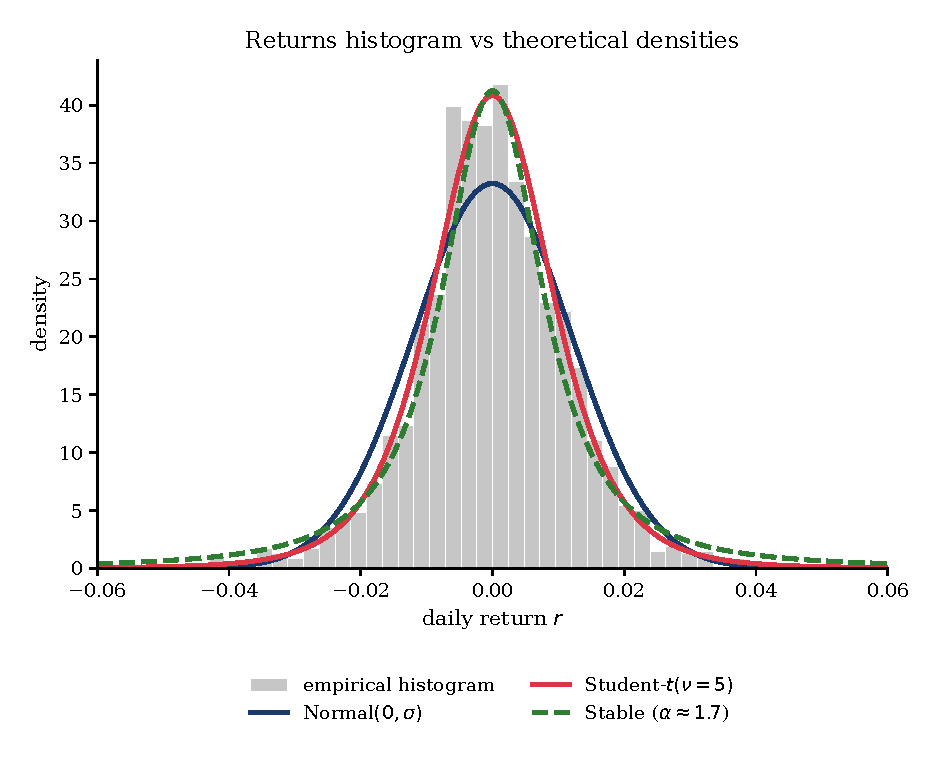
\includegraphics[width=0.85\linewidth]{sfm_sem_recap_density_overlay.pdf}
\end{block}
\end{column}
\begin{column}{0.37\textwidth}
\begin{itemize}\setlength{\itemsep}{0pt}
    \item \textbf{Cerințe:}
    \begin{itemize}\setlength{\itemsep}{0pt}
        \item Care densitate \textbf{subestimează} vârful (peak)?
        \item Care captează cel mai bine cozile?
        \item Histograma sugerează $S = 0$ sau $S \neq 0$?
        \item Care distribuție recomandați pentru VaR?
        \item Care este compromisul Student-$t$ vs stabilă?
    \end{itemize}
\end{itemize}
\end{column}
\end{columns}
\end{cminipage}
\vspace{0.05cm}
\quantlet{SFM\_sem\_recap\_plots}{https://colab.research.google.com/github/QuantLet/Stat_fin_markets/blob/master/Sem_recap/SFM_sem_recap_plots/SFM_sem_recap_plots.ipynb}
\end{frame}

\begin{frame}[shrink=25]{Exercițiul 22: Rezolvare}
\begin{cminipage}{0.95\textwidth}
\begin{exampleblock}{Rezolvare}
\begin{itemize}\setlength{\itemsep}{0pt}
    \item \textbf{1. Subestimarea vârfului:}
    \begin{itemize}\setlength{\itemsep}{0pt}
        \item Normala (curbă albastră) are vârful mai jos decât histograma
        \item Densitatea empirică este \textbf{mai ascuțită} decât cea normală $\Rightarrow$ leptokurtic
    \end{itemize}
    \item \textbf{2. Cozi:}
    \begin{itemize}\setlength{\itemsep}{0pt}
        \item Stabila (verde, linie punctată) are cozile cele mai groase
        \item Student-$t(\nu=5)$ (roșu) intermediar
        \item Normala (albastru) subestimează drastic cozile
    \end{itemize}
    \item \textbf{3. Asimetrie:}
    \begin{itemize}\setlength{\itemsep}{0pt}
        \item Histograma pare aproape simetrică $\Rightarrow$ $S \approx 0$
        \item Dacă ar fi $S < 0$, vârful histogramei s-ar deplasa spre dreapta
    \end{itemize}
    \item \textbf{4. Recomandare VaR:}
    \begin{itemize}\setlength{\itemsep}{0pt}
        \item Student-$t(\nu=5)$ sau stabilă cu $\alpha \approx 1{,}7$
        \item Normală strict nerecomandată pentru niveluri extreme (1\%, 0{,}1\%)
    \end{itemize}
    \item \textbf{5. Compromis Student-$t$ vs stabilă:}
    \begin{itemize}\setlength{\itemsep}{0pt}
        \item Student-$t$: momente finite, calibrare ușoară, integrare PDF existentă
        \item Stabilă: teoretic fundamentată (GCLT), dar varianță infinită pentru $\alpha < 2$
    \end{itemize}
\end{itemize}
\end{exampleblock}
\end{cminipage}
\end{frame}

\begin{frame}[shrink=30]{Exercițiul 23: Preț vs log-randament --- staționaritate}
\begin{cminipage}{0.95\textwidth}
\begin{columns}[T]
\begin{column}{0.62\textwidth}
\begin{block}{Enunț --- serii de timp, 500 zile}
\centering
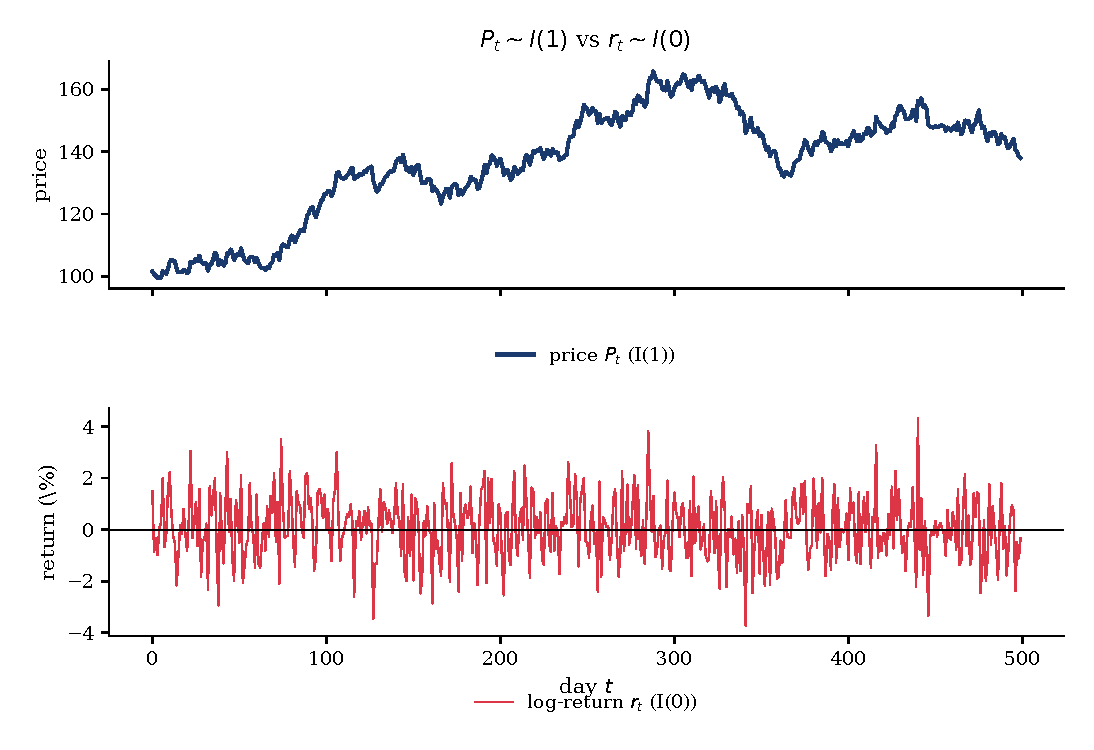
\includegraphics[width=\linewidth]{sfm_sem_recap_price_vs_return.pdf}
\end{block}
\end{column}
\begin{column}{0.35\textwidth}
\begin{itemize}\setlength{\itemsep}{0pt}
    \item \textbf{Tabel teste ADF ($H_0$: rădăcină unitară):}
    \begin{itemize}\setlength{\itemsep}{0pt}
        \item Preț $P_t$: ADF $= -1{,}24$, $p = 0{,}66$
        \item Log-rand. $r_t$: ADF $= -22{,}1$, $p < 0{,}001$
    \end{itemize}
    \item \textbf{Cerințe:}
    \begin{itemize}\setlength{\itemsep}{0pt}
        \item Care serie este $I(1)$? Care este $I(0)$?
        \item Interpretați rezultatele ADF
        \item Ce pericol apare dacă faceți regresie OLS pe prețuri?
        \item De ce log-randamentele sunt preferate în modele?
    \end{itemize}
\end{itemize}
\end{column}
\end{columns}
\end{cminipage}
\vspace{0.05cm}
\quantlet{SFM\_sem\_recap\_plots}{https://colab.research.google.com/github/QuantLet/Stat_fin_markets/blob/master/Sem_recap/SFM_sem_recap_plots/SFM_sem_recap_plots.ipynb}
\end{frame}

\begin{frame}[shrink=25]{Exercițiul 23: Rezolvare}
\begin{cminipage}{0.95\textwidth}
\begin{exampleblock}{Rezolvare}
\begin{itemize}\setlength{\itemsep}{0pt}
    \item \textbf{1. Clasificarea seriilor:}
    \begin{itemize}\setlength{\itemsep}{0pt}
        \item Prețul $P_t$: trend stocastic, varianță crescătoare $\Rightarrow$ \textbf{$I(1)$}
        \item Log-randamentul $r_t$: fluctuează în jur de zero $\Rightarrow$ \textbf{$I(0)$}
    \end{itemize}
    \item \textbf{2. Interpretare ADF:}
    \begin{itemize}\setlength{\itemsep}{0pt}
        \item Preț: $p = 0{,}66 > 0{,}05 \Rightarrow$ nu respingem $H_0$ (rădăcină unitară confirmată)
        \item Log-randament: $p < 0{,}001 \Rightarrow$ respingem $H_0$ (este staționar)
    \end{itemize}
    \item \textbf{3. Pericolul OLS pe prețuri:}
    \begin{itemize}\setlength{\itemsep}{0pt}
        \item \textbf{Regresie falsă} (spurious regression, Granger-Newbold 1974)
        \item $R^2$ artificial mare, $t$-statistici inflatate, predicții nevalide
        \item Reziduurile sunt autocorelate $\Rightarrow$ inferența OLS nevalidă
    \end{itemize}
    \item \textbf{4. De ce log-randamentele:}
    \begin{itemize}\setlength{\itemsep}{0pt}
        \item Staționare ($I(0)$) $\Rightarrow$ metodele statistice clasice se aplică
        \item Aditive în timp: $r_{0:T} = \sum r_t$
        \item Simetrice (loss/gain) și apropiate de normalitate (după mici transformări)
    \end{itemize}
\end{itemize}
\end{exampleblock}
\end{cminipage}
\end{frame}

\begin{frame}[shrink=30]{Exercițiul 24: Densități stabile --- impactul lui $\alpha$}
\begin{cminipage}{0.95\textwidth}
\begin{columns}[T]
\begin{column}{0.58\textwidth}
\begin{block}{Enunț --- densități stabile simetrice pentru diverse $\alpha$}
\centering
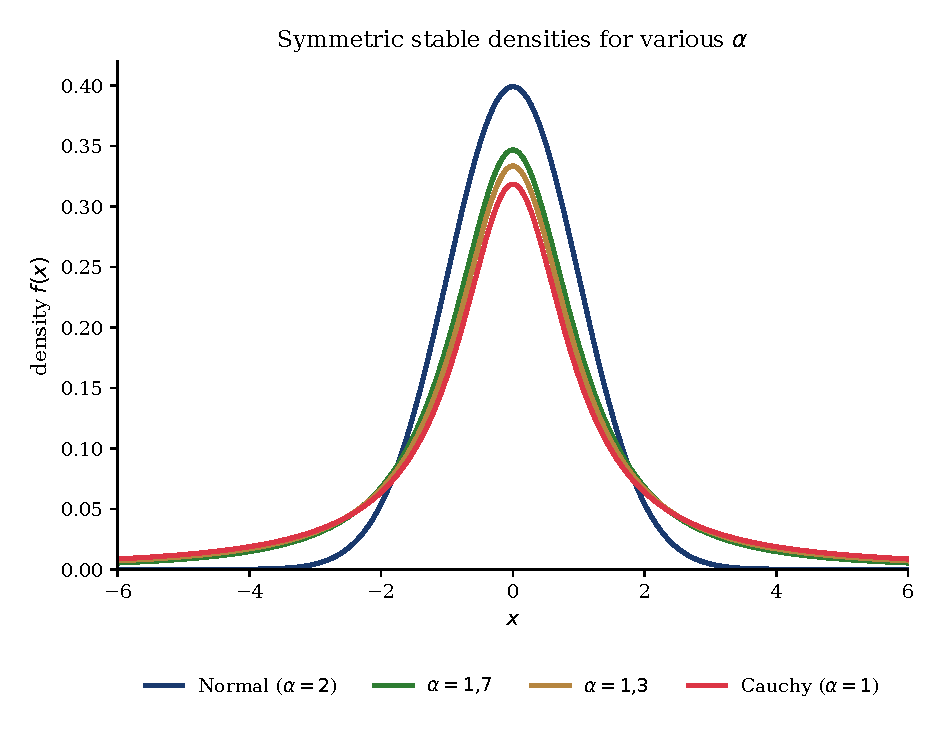
\includegraphics[width=0.85\linewidth]{sfm_sem_recap_stable_alpha.pdf}
\end{block}
\end{column}
\begin{column}{0.38\textwidth}
\begin{itemize}\setlength{\itemsep}{0pt}
    \item \textbf{Cerințe:}
    \begin{itemize}\setlength{\itemsep}{0pt}
        \item Cum se schimbă vârful când $\alpha$ scade de la $2$ la $1$?
        \item Cum se schimbă cozile?
        \item Pentru $\alpha = 1{,}3$: există varianța? Există media?
        \item Care distribuție ar modela cel mai bine Bitcoin? Gold?
        \item Ce se întâmplă cu Teorema Limită Centrală când $\alpha < 2$?
    \end{itemize}
\end{itemize}
\end{column}
\end{columns}
\end{cminipage}
\vspace{0.05cm}
\quantlet{SFM\_sem\_recap\_plots}{https://colab.research.google.com/github/QuantLet/Stat_fin_markets/blob/master/Sem_recap/SFM_sem_recap_plots/SFM_sem_recap_plots.ipynb}
\end{frame}

\begin{frame}[shrink=25]{Exercițiul 24: Rezolvare}
\begin{cminipage}{0.95\textwidth}
\begin{exampleblock}{Rezolvare}
\begin{itemize}\setlength{\itemsep}{0pt}
    \item \textbf{1. Evoluția vârfului ($\alpha: 2 \to 1$):}
    \begin{itemize}\setlength{\itemsep}{0pt}
        \item Vârful crește (densitatea devine mai ascuțită în jur de $0$)
        \item Concentrarea masei în jurul medianei crește
    \end{itemize}
    \item \textbf{2. Evoluția cozilor:}
    \begin{itemize}\setlength{\itemsep}{0pt}
        \item Cozile devin \textbf{progresiv mai groase}
        \item Cauchy ($\alpha=1$): decăderea lentă $|x|^{-2}$
        \item Normal ($\alpha=2$): decăderea rapidă $e^{-x^2/2}$
    \end{itemize}
    \item \textbf{3. Momente pentru $\alpha = 1{,}3$:}
    \begin{itemize}\setlength{\itemsep}{0pt}
        \item Momentele finite doar pentru ordin $p < \alpha = 1{,}3$
        \item Media ($p = 1 < 1{,}3$): \textbf{finită}
        \item Varianța ($p = 2 > 1{,}3$): \textbf{infinită}
    \end{itemize}
    \item \textbf{4. Recomandări de modelare:}
    \begin{itemize}\setlength{\itemsep}{0pt}
        \item Bitcoin: stabilă cu $\alpha \in [1{,}4, 1{,}7]$ (cozi foarte groase)
        \item Gold: $\alpha \in [1{,}8, 1{,}95]$ (aproape de normal, cozi moderate)
    \end{itemize}
    \item \textbf{5. CLT și $\alpha < 2$:}
    \begin{itemize}\setlength{\itemsep}{0pt}
        \item CLT clasic \textbf{nu se aplică} (varianță infinită)
        \item Se aplică GCLT (Generalized Central Limit Theorem)
        \item Suma iid stabile $\to$ stabilă (nu normală)
    \end{itemize}
\end{itemize}
\end{exampleblock}
\end{cminipage}
\end{frame}

%=============================================================================
% EXERCIȚII EXTINSE --- PARTEA VI
%=============================================================================
\section{Partea VI: Exerciții extinse și studii integrate}

\begin{frame}[shrink=25]{Exercițiul 25: Covarianță, corelație, beta de piață}
\begin{cminipage}{0.95\textwidth}
\begin{block}{Enunț}
\begin{itemize}\setlength{\itemsep}{0pt}
    \item Randamente zilnice pentru o acțiune $i$ și piața $m$ (eșantion $n = 252$):
    \begin{itemize}\setlength{\itemsep}{0pt}
        \item $\hat\mu_i = 0{,}08\%$, $\hat\sigma_i = 1{,}4\%$
        \item $\hat\mu_m = 0{,}04\%$, $\hat\sigma_m = 1{,}0\%$
        \item $\hat{\Cov}(r_i, r_m) = 0{,}000112$
    \end{itemize}
    \item \textbf{Cerințe:}
    \begin{itemize}\setlength{\itemsep}{0pt}
        \item Calculați coeficientul de corelație $\hat\rho_{i,m}$ folosind formula $\rho = \Cov/(\sigma_i \sigma_m)$
        \item Calculați coeficientul beta al acțiunii $\hat\beta_i = \Cov(r_i, r_m)/\Var(r_m)$
        \item Interpretați: acțiunea este agresivă ($\beta > 1$), defensivă ($\beta < 1$) sau neutră ($\beta = 1$) față de piață?
        \item Descompuneți varianța acțiunii în risc sistemic ($\beta^2 \sigma_m^2$) și risc idiosincratic (reziduu); calculați $R^2$ implicit
        \item Ce fracție din volatilitatea acțiunii este explicată de piață?
    \end{itemize}
\end{itemize}
\end{block}
\end{cminipage}
\end{frame}

\begin{frame}[shrink=25]{Exercițiul 25: Rezolvare}
\begin{cminipage}{0.95\textwidth}
\begin{exampleblock}{Rezolvare}
\begin{itemize}\setlength{\itemsep}{0pt}
    \item \textbf{1. Corelația} \quad $\rho_{i,m} = \dfrac{\Cov(r_i, r_m)}{\sigma_i \sigma_m}$
    \begin{itemize}\setlength{\itemsep}{0pt}
        \item $\hat\rho_{i,m} = 0{,}000112 / (0{,}014 \cdot 0{,}010) = 0{,}000112 / 0{,}00014 = \mathbf{0{,}80}$
        \item Corelație puternică pozitivă între acțiune și piață
    \end{itemize}
    \item \textbf{2. Beta} \quad $\beta_i = \dfrac{\Cov(r_i, r_m)}{\Var(r_m)} = \rho_{i,m} \cdot \dfrac{\sigma_i}{\sigma_m}$
    \begin{itemize}\setlength{\itemsep}{0pt}
        \item $\hat\beta_i = 0{,}000112 / (0{,}010)^2 = 0{,}000112 / 0{,}0001 = \mathbf{1{,}12}$
    \end{itemize}
    \item \textbf{3. Interpretare:}
    \begin{itemize}\setlength{\itemsep}{0pt}
        \item $\beta = 1{,}12 > 1 \Rightarrow$ acțiune \textbf{agresivă}
        \item Când piața crește 1\%, așteptăm acțiunea să crească $\sim 1{,}12\%$
    \end{itemize}
    \item \textbf{4. Descompunere varianță} \quad $\sigma_i^2 = \underbrace{\beta^2 \sigma_m^2}_{\text{sistemic}} + \underbrace{\sigma_\varepsilon^2}_{\text{idiosincratic}}$;\ $R^2 = \rho^2$
    \begin{itemize}\setlength{\itemsep}{0pt}
        \item Risc sistemic: $\beta^2 \sigma_m^2 = 1{,}12^2 \cdot 0{,}01^2 = 1{,}254 \cdot 10^{-4}$
        \item Risc idiosincratic: $\sigma_i^2 - \beta^2 \sigma_m^2 = 1{,}96 \cdot 10^{-4} - 1{,}254 \cdot 10^{-4} = 0{,}706 \cdot 10^{-4}$
        \item $R^2 = 0{,}80^2 = \mathbf{0{,}64}$
    \end{itemize}
    \item \textbf{5. Fracția explicată:}
    \begin{itemize}\setlength{\itemsep}{0pt}
        \item 64\% din varianța acțiunii este explicată de piață
        \item 36\% este risc specific firmei (diversificabil)
    \end{itemize}
\end{itemize}
\end{exampleblock}
\end{cminipage}
\end{frame}

\begin{frame}[shrink=30]{Exercițiul 26: Portofoliu de 2 active --- frontiera eficientă}
\begin{cminipage}{0.95\textwidth}
\begin{columns}[T]
\begin{column}{0.55\textwidth}
\begin{block}{Enunț --- frontiera eficientă}
\centering
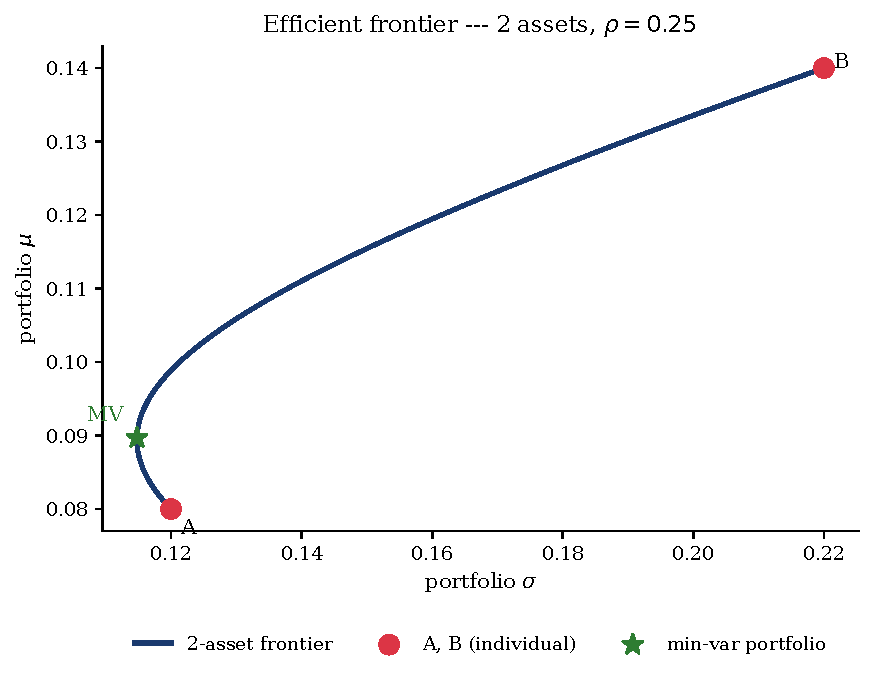
\includegraphics[width=\linewidth]{sfm_sem_recap_frontier.pdf}
\end{block}
\end{column}
\begin{column}{0.42\textwidth}
\begin{itemize}\setlength{\itemsep}{0pt}
    \item Date active:
    \begin{itemize}\setlength{\itemsep}{0pt}
        \item A: $\mu_A = 8\%$, $\sigma_A = 12\%$
        \item B: $\mu_B = 14\%$, $\sigma_B = 22\%$
        \item Corelație $\rho_{AB} = 0{,}25$
    \end{itemize}
    \item \textbf{Cerințe:}
    \begin{itemize}\setlength{\itemsep}{0pt}
        \item Scrieți formulele pentru $\mu_P$ și $\sigma_P^2$
        \item Calculați ponderea $w_A$ pentru portofoliul de varianță minimă (MV)
        \item Aflați $\mu_{MV}$ și $\sigma_{MV}$
        \item Explicați de ce MV are risc sub ambele active
        \item Ce rol joacă corelația $\rho$?
    \end{itemize}
\end{itemize}
\end{column}
\end{columns}
\end{cminipage}
\vspace{0.05cm}
\quantlet{SFM\_sem\_recap\_plots}{https://colab.research.google.com/github/QuantLet/Stat_fin_markets/blob/master/Sem_recap/SFM_sem_recap_plots/SFM_sem_recap_plots.ipynb}
\end{frame}

\begin{frame}[shrink=30]{Exercițiul 26: Rezolvare}
\begin{cminipage}{0.95\textwidth}
\begin{exampleblock}{Rezolvare}
\begin{itemize}\setlength{\itemsep}{0pt}
    \item \textbf{1. Formule portofoliu:}
    \begin{itemize}\setlength{\itemsep}{0pt}
        \item $\mu_P = w_A \mu_A + (1 - w_A) \mu_B$
        \item $\sigma_P^2 = w_A^2 \sigma_A^2 + (1 - w_A)^2 \sigma_B^2 + 2 w_A(1 - w_A) \sigma_A \sigma_B \rho$
    \end{itemize}
    \item \textbf{2. Ponderea MV (derivată = 0):}
    \begin{itemize}\setlength{\itemsep}{0pt}
        \item $w_A^{MV} = (\sigma_B^2 - \sigma_A \sigma_B \rho) / (\sigma_A^2 + \sigma_B^2 - 2 \sigma_A \sigma_B \rho)$
        \item $w_A^{MV} = (0{,}0484 - 0{,}12 \cdot 0{,}22 \cdot 0{,}25) / (0{,}0144 + 0{,}0484 - 0{,}0132)$
        \item $w_A^{MV} = 0{,}0418 / 0{,}0496 \approx \mathbf{0{,}843}$
    \end{itemize}
    \item \textbf{3. Randament și risc MV:}
    \begin{itemize}\setlength{\itemsep}{0pt}
        \item $\mu_{MV} = 0{,}843 \cdot 0{,}08 + 0{,}157 \cdot 0{,}14 = \mathbf{0{,}0894}$ ($8{,}94\%$)
        \item $\sigma_{MV}^2 = 0{,}843^2 \cdot 0{,}0144 + 0{,}157^2 \cdot 0{,}0484 + 2 \cdot 0{,}843 \cdot 0{,}157 \cdot 0{,}0066$
        \item $\sigma_{MV}^2 \approx 0{,}01242 \Rightarrow \sigma_{MV} \approx \mathbf{11{,}1\%}$
    \end{itemize}
    \item \textbf{4. Risc sub ambele active:}
    \begin{itemize}\setlength{\itemsep}{0pt}
        \item $\sigma_{MV} = 11{,}1\% < \sigma_A = 12\% < \sigma_B = 22\%$
        \item \textit{Interpretare:} portofoliul MV are \emph{mai puțin risc} decât oricare activ individual --- ``magia diversificării'' Markowitz (1952). Motiv: $\rho = 0{,}25 < 1$, mișcările nu sunt sincronizate
    \end{itemize}
    \item \textbf{5. Rolul corelației:}
    \begin{itemize}\setlength{\itemsep}{0pt}
        \item $\rho < 1$: diversificare efectivă, $\sigma_P$ redus
        \item $\rho = -1$: $\sigma_P = 0$ posibil (hedging perfect)
        \item $\rho = +1$: nicio diversificare
        \item \textit{Interpretare:} \textbf{capcana din crize} --- corelațiile cresc spre 1 când piețele cad sincron (``correlation breakdown''). Portofoliul ex-ante diversificat poate fi ex-post concentrat. Stress-test cu $\rho = 1$ pentru tail
    \end{itemize}
\end{itemize}
\end{exampleblock}
\end{cminipage}
\end{frame}

\begin{frame}[shrink=30]{Exercițiul 27: ACF pe pătrate --- efectul GARCH}
\begin{cminipage}{0.95\textwidth}
\begin{columns}[T]
\begin{column}{0.58\textwidth}
\begin{block}{Enunț --- ACF pe $r_t^2$, $n = 500$}
\centering
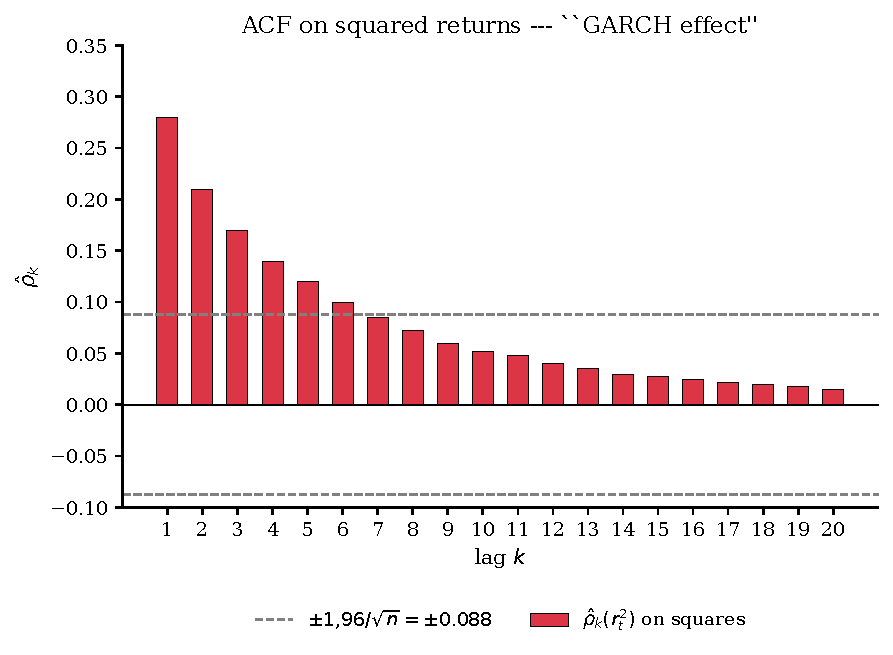
\includegraphics[width=\linewidth]{sfm_sem_recap_acf_squared.pdf}
\end{block}
\end{column}
\begin{column}{0.39\textwidth}
\begin{itemize}\setlength{\itemsep}{0pt}
    \item \textbf{Cerințe:}
    \begin{itemize}\setlength{\itemsep}{0pt}
        \item Identificați pattern-ul ACF pe $r_t^2$: descreștere lentă sau rapidă?
        \item Cum se compară cu ACF pe $r_t$ din Ex.~18 (unde doar lag 1 și 5 erau semnificative)?
        \item Ce fapta stilizată este evidențiată?
        \item Este compatibil cu EMH slabă? De ce?
        \item Ce model statistic se recomandă pentru modelarea acestui comportament?
    \end{itemize}
\end{itemize}
\end{column}
\end{columns}
\end{cminipage}
\vspace{0.05cm}
\quantlet{SFM\_sem\_recap\_plots}{https://colab.research.google.com/github/QuantLet/Stat_fin_markets/blob/master/Sem_recap/SFM_sem_recap_plots/SFM_sem_recap_plots.ipynb}
\end{frame}

\begin{frame}[shrink=40]{Exercițiul 27: Rezolvare}
\begin{cminipage}{0.95\textwidth}
\begin{exampleblock}{Rezolvare}
\begin{itemize}\setlength{\itemsep}{0pt}
    \item \textbf{1. Pattern ACF pe $r_t^2$:}
    \begin{itemize}\setlength{\itemsep}{0pt}
        \item Autocorelații toate pozitive, descreștere hiperbolică până la lag $20+$
        \item Toate lag-urile $1$--$15$ semnificative
        \item \textit{Interpretare:} pattern universal pe orice activ financiar. Decay hiperbolic (nu exponențial) indică \emph{long memory}, mai mult decât AR(1) clasic
    \end{itemize}
    \item \textbf{2. Comparație cu $r_t$:}
    \begin{itemize}\setlength{\itemsep}{0pt}
        \item $r_t$: doar 1--2 lag-uri marginal semnificative
        \item $r_t^2$: memorie lungă clară
        \item \textit{Interpretare:} dichotomia este \emph{cea mai robustă} fapta stilizată. Randamentele sunt \emph{aproape} necorelate liniar, dar magnitudinile persistă. Asta motivează GARCH
    \end{itemize}
    \item \textbf{3. Fapta stilizată} \quad \textbf{Clustering de volatilitate} (Mandelbrot 1963)
    \begin{itemize}\setlength{\itemsep}{0pt}
        \item Zile cu vol mare urmate de zile cu vol mare; regimuri grupate
        \item \textit{Interpretare:} consecință economică: riscul se acumulează în ``regimuri'' (oct.\ 2008, mar.\ 2020). Modelele Black-Scholes cu $\sigma$ constantă sunt sistematic greșite în crize
    \end{itemize}
    \item \textbf{4. Compatibilitate cu EMH slabă:}
    \begin{itemize}\setlength{\itemsep}{0pt}
        \item \textbf{Da, compatibil.} EMH slabă cere doar impredictibilitatea \emph{randamentelor}
        \item Volatilitatea predictibilă $\ne$ randament predictibil
        \item \textit{Interpretare:} poți \emph{prezice riscul} (volatility forecasting), \emph{nu direcția}. Bază pentru opțiuni dinamice (GARCH option models, Heston SV)
    \end{itemize}
    \item \textbf{5. Model recomandat:}
    \begin{itemize}\setlength{\itemsep}{0pt}
        \item ARCH/GARCH (Engle 1982, Bollerslev 1986)
        \item EGARCH, GJR-GARCH pentru leverage effect
        \item Realized Volatility / HAR pe date intra-zilnice
        \item \textit{Interpretare:} GARCH(1,1) ``go-to'' didactic; HAR-RV standard industrial; rough volatility ($H < 0{,}5$) frontiera modernă (Gatheral et al.\ 2018)
    \end{itemize}
\end{itemize}
\end{exampleblock}
\end{cminipage}
\end{frame}

\begin{frame}[shrink=30]{Exercițiul 28: Estimatorul Hill pentru indicele de coadă}
\begin{cminipage}{0.95\textwidth}
\begin{columns}[T]
\begin{column}{0.58\textwidth}
\begin{block}{Enunț --- Hill plot pe coada stângă}
\centering
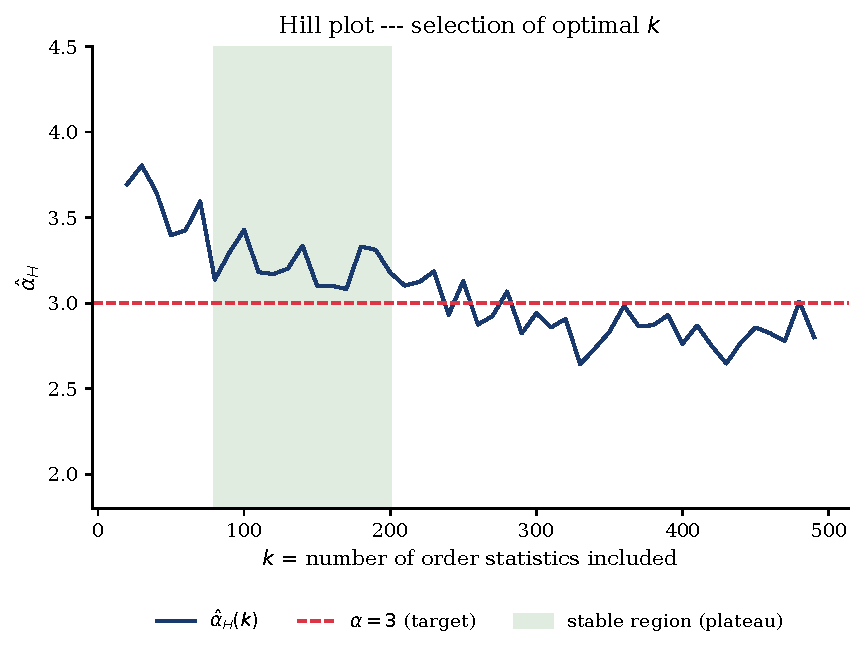
\includegraphics[width=0.85\linewidth]{sfm_sem_recap_hill.pdf}
\end{block}
\end{column}
\begin{column}{0.39\textwidth}
\begin{itemize}\setlength{\itemsep}{0pt}
    \item Formula estimatorului Hill:
    \begin{itemize}\setlength{\itemsep}{0pt}
        \item $\hat\alpha_H(k) = \left[\frac{1}{k}\sum_{i=1}^{k} \ln(X_{(i)}/X_{(k+1)})\right]^{-1}$
    \end{itemize}
    \item \textbf{Cerințe:}
    \begin{itemize}\setlength{\itemsep}{0pt}
        \item Interpretați forma graficului: de ce estimatorul variază cu $k$?
        \item Care este zona de ``plateau'' și ce $\hat\alpha$ se alege?
        \item Ce problemă apare la $k$ mic? Dar la $k$ mare?
        \item Cu $\hat\alpha \approx 3$, ce distribuție ar modela cozile?
    \end{itemize}
\end{itemize}
\end{column}
\end{columns}
\end{cminipage}
\vspace{0.05cm}
\quantlet{SFM\_sem\_recap\_plots}{https://colab.research.google.com/github/QuantLet/Stat_fin_markets/blob/master/Sem_recap/SFM_sem_recap_plots/SFM_sem_recap_plots.ipynb}
\end{frame}

\begin{frame}[shrink=25]{Exercițiul 28: Rezolvare}
\begin{cminipage}{0.95\textwidth}
\begin{exampleblock}{Rezolvare}
\begin{itemize}\setlength{\itemsep}{0pt}
    \item \textbf{1. Forma graficului} \quad $\hat\alpha_H(k) = \left[\dfrac{1}{k}\sum_{i=1}^{k} \ln(X_{(i)}/X_{(k+1)})\right]^{-1}$
    \begin{itemize}\setlength{\itemsep}{0pt}
        \item $k$ mic: volatilitate mare (prea puține puncte extreme $\Rightarrow$ varianță de estimare mare)
        \item $k$ mare: bias (se includ puncte din corpul distribuției, nu doar coadă)
        \item Zona de plateau: stabilă între cele două erori
    \end{itemize}
    \item \textbf{2. Plateau și alegere:}
    \begin{itemize}\setlength{\itemsep}{0pt}
        \item Zona verde ($k \in [80, 200]$) prezintă valori stabile $\hat\alpha \approx 3{,}0$
        \item Se alege $k$ din mijlocul plateau-ului ($k \approx 140$)
    \end{itemize}
    \item \textbf{3. Probleme la extreme:}
    \begin{itemize}\setlength{\itemsep}{0pt}
        \item $k$ mic: estimare zgomotoasă, intervale de încredere largi
        \item $k$ mare: corpul distribuției contaminează estimarea cozii
        \item Compromis bias-variance clasic
    \end{itemize}
    \item \textbf{4. Modelarea cozilor cu $\hat\alpha \approx 3$:}
    \begin{itemize}\setlength{\itemsep}{0pt}
        \item Pareto sau GPD (Generalized Pareto Distribution): $\bar F(x) \sim C x^{-3}$
        \item Student-$t$ cu $\nu \approx 3$ (momente de ordin $< 3$ finite, ordin $\ge 3$ infinite)
        \item Varianța este finită ($\alpha > 2$) dar kurtosis infinit
    \end{itemize}
\end{itemize}
\end{exampleblock}
\end{cminipage}
\end{frame}

\begin{frame}[shrink=25]{Exercițiul 29: Test CUSUM --- rupturi structurale}
\begin{cminipage}{0.95\textwidth}
\begin{columns}[T]
\begin{column}{0.58\textwidth}
\begin{block}{Enunț --- CUSUM pe 500 zile}
\centering
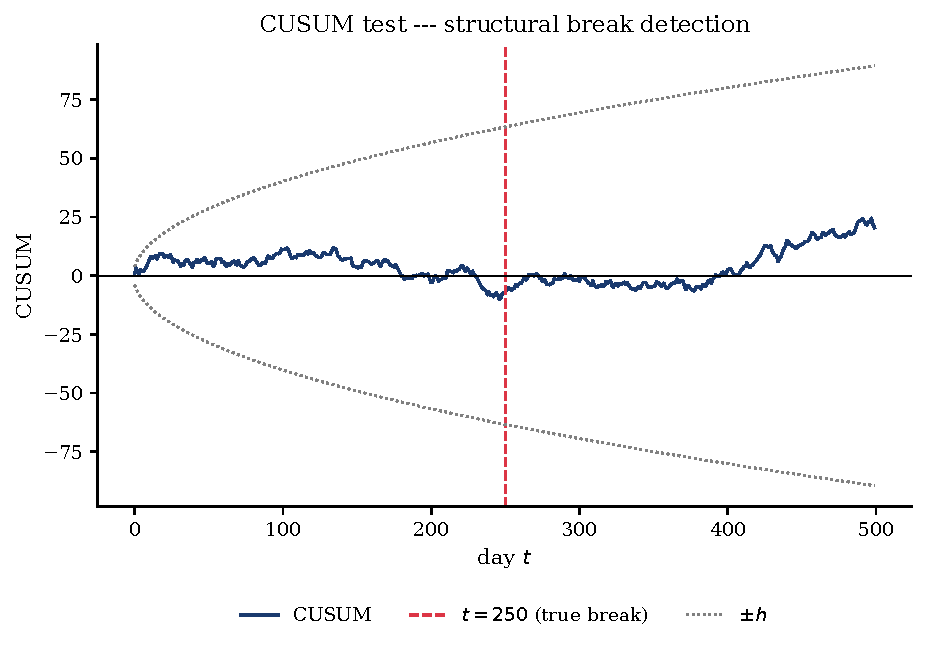
\includegraphics[width=\linewidth]{sfm_sem_recap_cusum.pdf}
\end{block}
\end{column}
\begin{column}{0.39\textwidth}
\begin{itemize}\setlength{\itemsep}{0pt}
    \item Statistica CUSUM:
    \begin{itemize}\setlength{\itemsep}{0pt}
        \item $S_t = \sum_{i=1}^{t}(x_i - \mu_0)$
        \item Limite: $\pm h\sqrt{t}$
    \end{itemize}
    \item \textbf{Cerințe:}
    \begin{itemize}\setlength{\itemsep}{0pt}
        \item Identificați momentul rupturii aparente în grafic
        \item De ce CUSUM depășește limita superioară după un anumit $t$?
        \item Ce fel de schimbare este detectată: în medie, în varianță sau ambele?
        \item Ce implicații are o ruptură pentru modelarea seriei?
        \item Ce alternative există pentru serii cu regim-switching?
    \end{itemize}
\end{itemize}
\end{column}
\end{columns}
\end{cminipage}
\vspace{0.05cm}
\quantlet{SFM\_sem\_recap\_plots}{https://colab.research.google.com/github/QuantLet/Stat_fin_markets/blob/master/Sem_recap/SFM_sem_recap_plots/SFM_sem_recap_plots.ipynb}
\end{frame}

\begin{frame}[shrink=30]{Exercițiul 29: Rezolvare}
\begin{cminipage}{0.95\textwidth}
\begin{exampleblock}{Rezolvare}
\begin{itemize}\setlength{\itemsep}{0pt}
    \item \textbf{1. Momentul rupturii:}
    \begin{itemize}\setlength{\itemsep}{0pt}
        \item CUSUM oscilează în jur de 0 până la $t \approx 250$
        \item După $t = 250$, deviază sistematic pozitiv $\Rightarrow$ semnal de ruptură
        \item Depășește limita superioară $+h\sqrt{t}$ în jurul $t \approx 350$
        \item \textit{Interpretare:} CUSUM cumulează deviațiile de la $\mu_0$. O ruptură produce pantă constantă; detecția vine cu decalaj proporțional cu mărimea schimbării
    \end{itemize}
    \item \textbf{2. De ce depășește} \quad media sare de la $\mu_0 = 0$ la $\mu_1 = 0{,}15$
    \begin{itemize}\setlength{\itemsep}{0pt}
        \item Cumulare sistematică de deviații pozitive $\Rightarrow$ $S_t$ crește linear
        \item \textit{Interpretare:} timpul de detecție depinde de $|\mu_1 - \mu_0|/\sigma$ și pragul $h$. Trade-off: $h$ mic $\to$ false alarms; $h$ mare $\to$ detecție lentă
    \end{itemize}
    \item \textbf{3. Ce schimbare detectează:}
    \begin{itemize}\setlength{\itemsep}{0pt}
        \item CUSUM clasic detectează schimbări în \textbf{medie}
        \item Pentru varianță: CUSUM pe $|x_t|$ sau $x_t^2$
        \item \textit{Interpretare:} ruptură în $\mu$ poate semnala schimbare regim macro (politică monetară, criză); în $\sigma$, schimbare regim de risc
    \end{itemize}
    \item \textbf{4. Implicații pentru modelare:}
    \begin{itemize}\setlength{\itemsep}{0pt}
        \item Parametri constanti nu mai sunt valizi $\Rightarrow$ rolling estimation
        \item \textit{Interpretare:} ignorarea rupturilor cauzează backtesting greșit. ``Lucas critique'' financiar: parametrii pre-ruptură nu se aplică post-ruptură
    \end{itemize}
    \item \textbf{5. Alternative regim-switching:}
    \begin{itemize}\setlength{\itemsep}{0pt}
        \item Markov Switching Models (Hamilton 1989), TAR/SETAR
        \item Structural break tests: Bai-Perron, Chow, Quandt-Andrews
        \item \textit{Interpretare:} Markov-switching elegant teoretic; TAR/SETAR pragmatic; Bai-Perron pentru \emph{multiple} rupturi. Modern: change-point bayesian online
    \end{itemize}
\end{itemize}
\end{exampleblock}
\end{cminipage}
\end{frame}

\begin{frame}[shrink=25]{Exercițiul 30: Efectul de leverage}
\begin{cminipage}{0.95\textwidth}
\begin{columns}[T]
\begin{column}{0.55\textwidth}
\begin{block}{Enunț --- scatter $r_t$ vs $\sigma_{t+1}$}
\centering
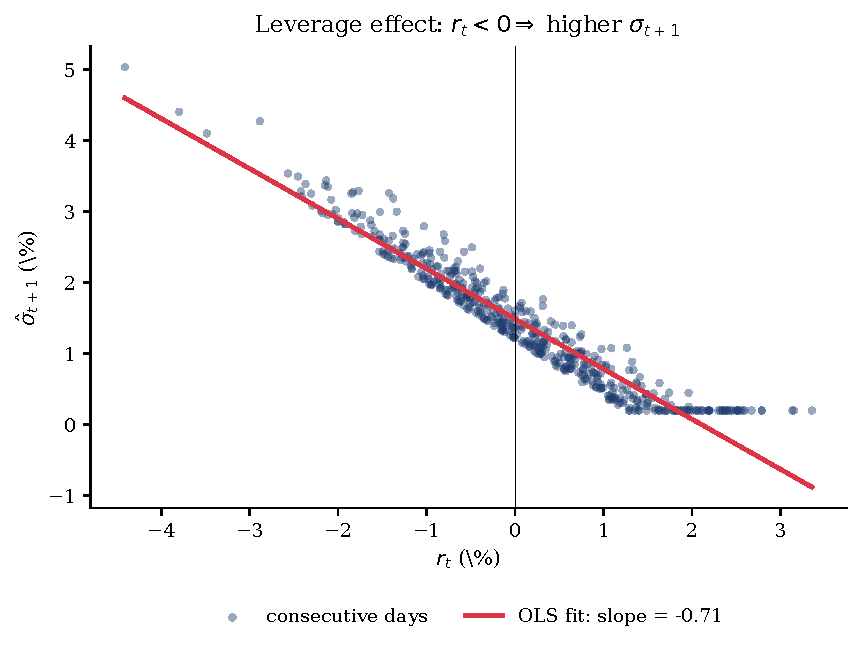
\includegraphics[width=\linewidth]{sfm_sem_recap_leverage.pdf}
\end{block}
\end{column}
\begin{column}{0.42\textwidth}
\begin{itemize}\setlength{\itemsep}{0pt}
    \item \textbf{Cerințe:}
    \begin{itemize}\setlength{\itemsep}{0pt}
        \item Descrieți panta regresiei: este pozitivă sau negativă?
        \item Ce fapta stilizată reprezintă acest pattern?
        \item Interpretare economică: de ce pierderile mari prezic volatilitate mai mare?
        \item Care model GARCH specific captează acest efect?
        \item Cum se distinge leverage effect de clustering de volatilitate?
    \end{itemize}
\end{itemize}
\end{column}
\end{columns}
\end{cminipage}
\vspace{0.05cm}
\quantlet{SFM\_sem\_recap\_plots}{https://colab.research.google.com/github/QuantLet/Stat_fin_markets/blob/master/Sem_recap/SFM_sem_recap_plots/SFM_sem_recap_plots.ipynb}
\end{frame}

\begin{frame}[shrink=25]{Exercițiul 30: Rezolvare}
\begin{cminipage}{0.95\textwidth}
\begin{exampleblock}{Rezolvare}
\begin{itemize}\setlength{\itemsep}{0pt}
    \item \textbf{1. Panta regresiei:}
    \begin{itemize}\setlength{\itemsep}{0pt}
        \item \textbf{Negativă}: randamente negative $\Rightarrow$ volatilitate crescută a doua zi
        \item Randamentele pozitive au un impact mai mic asupra volatilității viitoare
    \end{itemize}
    \item \textbf{2. Fapta stilizată:}
    \begin{itemize}\setlength{\itemsep}{0pt}
        \item \textbf{Leverage effect} (Black, 1976; Christie, 1982)
        \item Răspuns asimetric al volatilității la șocuri pozitive vs negative
    \end{itemize}
    \item \textbf{3. Interpretare economică:}
    \begin{itemize}\setlength{\itemsep}{0pt}
        \item Scăderi mari ale prețului $\Rightarrow$ creștere a raportului debt/equity
        \item Companii cu datorii mari devin mai riscante după o scădere
        \item ``Volatility feedback'': volatilitate mai mare $\Rightarrow$ prima de risc mai mare $\Rightarrow$ preț mai jos
    \end{itemize}
    \item \textbf{4. Modele GARCH care captează:}
    \begin{itemize}\setlength{\itemsep}{0pt}
        \item EGARCH (Nelson, 1991): $\ln \sigma_t^2 = \omega + \alpha |z_{t-1}| + \gamma z_{t-1}$
        \item GJR-GARCH (Glosten-Jagannathan-Runkle, 1993): termen suplimentar pentru $\varepsilon_{t-1} < 0$
        \item TGARCH (Zakoian, 1994)
    \end{itemize}
    \item \textbf{5. Distincție de clustering:}
    \begin{itemize}\setlength{\itemsep}{0pt}
        \item Clustering: persistență în amplitudine, fără direcție
        \item Leverage: asimetrie legată de semnul randamentului
    \end{itemize}
\end{itemize}
\end{exampleblock}
\end{cminipage}
\end{frame}

\begin{frame}[shrink=25]{Exercițiul 31: Monte Carlo --- 100 traiectorii GBM}
\begin{cminipage}{0.95\textwidth}
\begin{columns}[T]
\begin{column}{0.58\textwidth}
\begin{block}{Enunț --- simulări GBM cu $\mu = 10\%$, $\sigma = 20\%$}
\centering
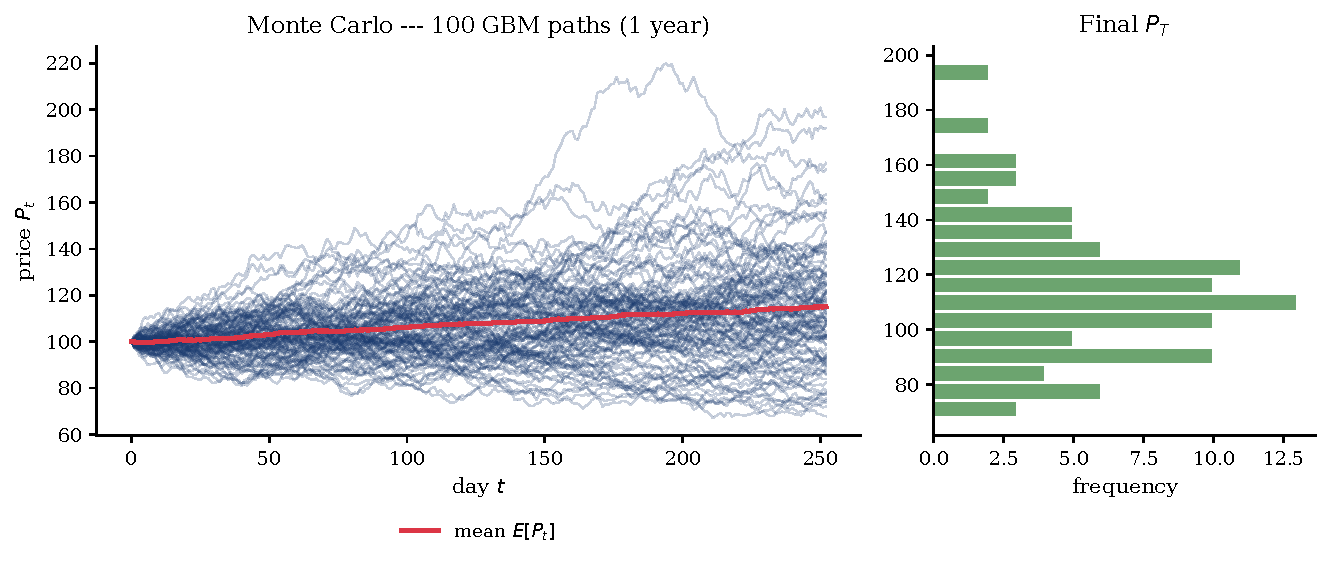
\includegraphics[width=\linewidth]{sfm_sem_recap_monte_carlo.pdf}
\end{block}
\end{column}
\begin{column}{0.39\textwidth}
\begin{itemize}\setlength{\itemsep}{0pt}
    \item Modelul: $dP_t = \mu P_t\, dt + \sigma P_t\, dW_t$
    \item $P_0 = 100$, orizont $T = 1$ an (252 zile)
    \item \textbf{Cerințe:}
    \begin{itemize}\setlength{\itemsep}{0pt}
        \item Interpretați dispersia traiectoriilor la $T = 1$
        \item Distribuția lui $P_T$ este normală sau log-normală?
        \item Calculați $\E[P_T]$ și $\Var(P_T)$ teoretice
        \item Ce reprezintă coada stângă a histogramei?
        \item Cum se calculează VaR 5\% prin Monte Carlo?
    \end{itemize}
\end{itemize}
\end{column}
\end{columns}
\end{cminipage}
\vspace{0.05cm}
\quantlet{SFM\_sem\_recap\_plots}{https://colab.research.google.com/github/QuantLet/Stat_fin_markets/blob/master/Sem_recap/SFM_sem_recap_plots/SFM_sem_recap_plots.ipynb}
\end{frame}

\begin{frame}[shrink=25]{Exercițiul 31: Rezolvare}
\begin{cminipage}{0.95\textwidth}
\begin{exampleblock}{Rezolvare}
\begin{itemize}\setlength{\itemsep}{0pt}
    \item \textbf{1. Soluția SDE GBM} \quad $P_t = P_0 \exp\left((\mu - \sigma^2/2)t + \sigma W_t\right)$
    \begin{itemize}\setlength{\itemsep}{0pt}
        \item Dispersia crește cu $\sqrt{t}$ (proporțional cu $\sigma$)
        \item La $T = 1$, $P_T \in [\sim 60, \sim 160]$ (asimetric)
    \end{itemize}
    \item \textbf{2. Distribuția lui $P_T$} \quad log-normală: $\ln P_T \sim \mathcal{N}\!\left((\mu - \sigma^2/2)T,\; \sigma^2 T\right)$
    \begin{itemize}\setlength{\itemsep}{0pt}
        \item Asimetrică spre dreapta (cozi mai grele la valori mari)
    \end{itemize}
    \item \textbf{3. Momente teoretice} \quad $\E[P_T] = P_0 e^{\mu T}$;\ $\Var(P_T) = P_0^2 e^{2\mu T}(e^{\sigma^2 T} - 1)$
    \begin{itemize}\setlength{\itemsep}{0pt}
        \item $\E[P_T] = 100 \cdot e^{0{,}10} = \mathbf{110{,}5}$
        \item $\Var(P_T) = 100^2 \cdot 1{,}221 \cdot 0{,}0408 \approx 499$
        \item $\sigma_{P_T} \approx 22{,}3$ (aproximativ $\sigma$ anualizat)
    \end{itemize}
    \item \textbf{4. Coada stângă:}
    \begin{itemize}\setlength{\itemsep}{0pt}
        \item Traiectorii cu pierderi mari (rare)
        \item Input pentru calculul VaR
    \end{itemize}
    \item \textbf{5. VaR Monte Carlo:}
    \begin{itemize}\setlength{\itemsep}{0pt}
        \item Rulează $N$ traiectorii, colectează $\{P_T^{(i)}\}$
        \item Sortează crescător, ia cuantila 5\% empirică
        \item Avantaj: nu presupune distribuție parametrică specifică; captează neliniarități
    \end{itemize}
\end{itemize}
\end{exampleblock}
\end{cminipage}
\end{frame}

\begin{frame}[shrink=25]{Exercițiul 33: Test Kolmogorov--Smirnov (goodness of fit)}
\begin{cminipage}{0.95\textwidth}
\begin{block}{Enunț --- teste KS pe randamente S\&P 500, $n = 2.500$}
\small
\renewcommand{\arraystretch}{1.2}
\begin{center}
\begin{tabular}{lccc}
\toprule
\textbf{Distribuție testată} & \textbf{Statistica $D$} & \textbf{$p$-value} & \textbf{Decizie la 5\%} \\
\midrule
$\mathcal{N}(\hat\mu, \hat\sigma^2)$ & $0{,}052$ & $< 0{,}001$ & \textcolor{Crimson}{Respinsă} \\
Student-$t(\hat\nu = 5{,}2)$ & $0{,}018$ & $0{,}423$ & \textcolor{Forest}{Acceptată} \\
Laplace$(\hat\mu, \hat b)$ & $0{,}037$ & $0{,}015$ & \textcolor{Crimson}{Respinsă} \\
Stable$(\hat\alpha = 1{,}76, \ldots)$ & $0{,}014$ & $0{,}712$ & \textcolor{Forest}{Acceptată} \\
\bottomrule
\end{tabular}
\end{center}
Valoare critică: $D_{0{,}05} \approx 1{,}36/\sqrt{n} \approx 0{,}027$.
\end{block}
\begin{itemize}\setlength{\itemsep}{0pt}
    \item \textbf{Cerințe:}
    \begin{itemize}\setlength{\itemsep}{0pt}
        \item Care distribuții sunt respinse? Care sunt acceptate?
        \item Compare statistica $D$ cu valoarea critică --- de ce e utilă?
        \item Cum interpretați faptul că atât Student-$t$ cât și Stable sunt acceptate?
        \item Pentru VaR, care distribuție recomandați dintre cele acceptate?
        \item Limitările testului KS pentru eșantioane mari
    \end{itemize}
\end{itemize}
\end{cminipage}
\end{frame}

\begin{frame}[shrink=35]{Exercițiul 33: Rezolvare}
\begin{cminipage}{0.95\textwidth}
\begin{exampleblock}{Rezolvare}
\begin{itemize}\setlength{\itemsep}{0pt}
    \item \textbf{1. Distribuții acceptate/respinse:}
    \begin{itemize}\setlength{\itemsep}{0pt}
        \item \textbf{Respinse} ($p < 0{,}05$): Normal, Laplace
        \item \textbf{Acceptate}: Student-$t(\nu = 5{,}2)$, Stable($\alpha = 1{,}76$)
        \item \textit{Interpretare:} Normala respinsă (cum era de așteptat); Laplace respinsă pentru că presupune cozi exponențiale (mai subțiri decât empiric); $t$ și Stable trec testul
    \end{itemize}
    \item \textbf{2. Statistica $D$ vs valoare critică} \quad $D = \sup_x|F_n(x) - F(x)|$;\ $D_{0{,}05} \approx 1{,}358/\sqrt n \approx 0{,}027$
    \begin{itemize}\setlength{\itemsep}{0pt}
        \item Normal: $D = 0{,}052 > 0{,}027 \Rightarrow$ respingere
        \item Student-$t$: $D = 0{,}018 < 0{,}027 \Rightarrow$ acceptare
        \item \textit{Interpretare:} $D$ măsoară \emph{maximul deviației} CDF empirică vs.\ teoretică. Avantaj vs.\ JB: nu necesită distribuție specifică --- folosibil pentru orice $F$
    \end{itemize}
    \item \textbf{3. Ambele acceptate:}
    \begin{itemize}\setlength{\itemsep}{0pt}
        \item KS nu discriminează între modele apropiate în corp
        \item Diferența ar apărea în cozi (KS are putere mică la extreme)
        \item \textit{Interpretare:} acceptarea ambele modele NU înseamnă că ele sunt ``corecte'', ci că la rezoluție KS sunt indistinguibile. Pentru risc, alegerea contează (Stable mai conservatoare la $0{,}1\%$)
    \end{itemize}
    \item \textbf{4. Recomandare pentru VaR:}
    \begin{itemize}\setlength{\itemsep}{0pt}
        \item Nivel $5\%$ $\Rightarrow$ Student-$t$ suficient
        \item Nivel $0{,}1\%$ sau stres $\Rightarrow$ Stable (mai conservatoare în cozi)
        \item \textit{Interpretare:} Basel III impune VaR la $1\%$ pe 10 zile + ES la $2{,}5\%$. Pentru aceste niveluri, $t(\nu = 5)$ este standard industrial; Stable e ``stress add-on''
    \end{itemize}
    \item \textbf{5. Limitările KS:}
    \begin{itemize}\setlength{\itemsep}{0pt}
        \item Pentru $n$ mare, KS respinge aproape orice distribuție parametrică
        \item Anderson--Darling preferat pentru putere în cozi
        \item Cu parametri estimați, nivelul efectiv $\ne$ nominal
        \item \textit{Interpretare:} KS este test brut --- pentru analiză cozilor folosiți AD sau Cramér--von Mises. KS este excelent ca \emph{primă verificare}, nu ca decizie finală
    \end{itemize}
\end{itemize}
\end{exampleblock}
\end{cminipage}
\end{frame}

\begin{frame}[shrink=25]{Exercițiul 34: Backtest strategie de momentum}
\begin{cminipage}{0.95\textwidth}
\begin{block}{Enunț --- rezultat backtest strategie pe S\&P 500 (2010--2024)}
\small
\renewcommand{\arraystretch}{1.2}
\begin{center}
\begin{tabular}{lccc}
\toprule
\textbf{Indicator} & \textbf{Strategie momentum} & \textbf{Buy \& Hold} & \textbf{Diferență} \\
\midrule
Randament anual & $14{,}8\%$ & $12{,}5\%$ & $+2{,}3\%$ \\
Volatilitate anuală & $18{,}2\%$ & $15{,}4\%$ & $+2{,}8\%$ \\
Sharpe (cu $R_f = 2\%$) & $0{,}70$ & $0{,}68$ & $+0{,}02$ \\
Maximum Drawdown & $-24{,}5\%$ & $-34{,}0\%$ & $+9{,}5\%$ \\
Calmar & $0{,}60$ & $0{,}37$ & $+0{,}23$ \\
Număr tranzacții/an & $22$ & $0$ & --- \\
Cost tranzacție/an (0,1\%) & $-2{,}2\%$ & $0$ & $-2{,}2\%$ \\
Randament \textbf{net} & $\mathbf{12{,}6\%}$ & $\mathbf{12{,}5\%}$ & $\mathbf{+0{,}1\%}$ \\
\bottomrule
\end{tabular}
\end{center}
\end{block}
\begin{itemize}\setlength{\itemsep}{0pt}
    \item \textbf{Cerințe:}
    \begin{itemize}\setlength{\itemsep}{0pt}
        \item Strategia pare să câștige brut? După costuri?
        \item Ce criteriu arată clar superioritatea momentum?
        \item Este compatibil cu EMH slabă?
        \item Care este ``capcana backtesting'' (survivorship bias, overfitting)?
        \item Recomandare finală: merită strategia implementată?
    \end{itemize}
\end{itemize}
\end{cminipage}
\end{frame}

\begin{frame}[shrink=30]{Exercițiul 34: Rezolvare}
\begin{cminipage}{0.95\textwidth}
\begin{exampleblock}{Rezolvare}
\begin{itemize}\setlength{\itemsep}{0pt}
    \item \textbf{1. Performanță brută vs netă:}
    \begin{itemize}\setlength{\itemsep}{0pt}
        \item Brută: $+2{,}3\%$ în favoarea momentum;\ netă: $+0{,}1\%$ după costuri
        \item \textit{Interpretare:} ``alpha decay'' --- $2{,}3\%$ alfă anulată cu $2{,}2\%$ costuri. Fără execuție low-cost (dark pools, broker instituțional) strategia nu e profitabilă
    \end{itemize}
    \item \textbf{2. Criteriu dominant:}
    \begin{itemize}\setlength{\itemsep}{0pt}
        \item MDD: $-24{,}5\%$ vs $-34\%$;\ Calmar: $0{,}60$ vs $0{,}37$
        \item \textit{Interpretare:} pe Sharpe abia diferență; pe Calmar momentum e dominant. Trend-following filtrează crize $\Rightarrow$ investitorul cu aversiune la pierdere preferă momentum chiar și fără alfa net
    \end{itemize}
    \item \textbf{3. Compatibilitate EMH:}
    \begin{itemize}\setlength{\itemsep}{0pt}
        \item Net: nu bate piața semnificativ $\Rightarrow$ compatibil cu EMH slabă
        \item \textit{Interpretare:} EMH ``salvată'' de costuri --- AMH în acțiune. Strategia funcționa în anii $80$--$90$ când costurile erau $20$--$50$ bp; astăzi e erodată
    \end{itemize}
    \item \textbf{4. Capcane backtesting:}
    \begin{itemize}\setlength{\itemsep}{0pt}
        \item Survivorship bias, overfitting, look-ahead bias, $p$-hacking
        \item \textit{Interpretare:} aceste capcane explică de ce $80\%+$ din strategiile ``câștigătoare'' în backtesting eșuează în producție. Soluție: walk-forward validation, deflated Sharpe (Bailey \& López de Prado 2014)
    \end{itemize}
    \item \textbf{5. Recomandare:}
    \begin{itemize}\setlength{\itemsep}{0pt}
        \item Marginal superior în MDD/Calmar, cost ridicat
        \item Implementare doar cu avers la drawdown, execuție low-cost, validare OOS
        \item \textit{Interpretare:} pentru retail nu merită; pentru fond mare cu execuție profesională, da. Lecție: \emph{transaction cost scaling} crucial în backtesting
    \end{itemize}
\end{itemize}
\end{exampleblock}
\end{cminipage}
\end{frame}

\begin{frame}[shrink=25]{Exercițiul 36: Value-at-Risk la orizonturi multiple}
\begin{cminipage}{0.95\textwidth}
\begin{block}{Enunț}
\begin{itemize}\setlength{\itemsep}{0pt}
    \item Un portofoliu de \$5M are randament zilnic cu $\mu = 0$, $\sigma_{\text{zi}} = 1\%$ sub ipoteza i.i.d.~normală.
    \item \textbf{Cerințe:}
    \begin{itemize}\setlength{\itemsep}{0pt}
        \item Calculați VaR zilnic 1\% folosind $z_{0{,}01} = 2{,}326$
        \item Calculați VaR la orizont 10 zile folosind regula $\sqrt{T}$
        \item Calculați VaR la orizont 1 lună (22 zile)
        \item Comentați cum se scalează VaR cu orizontul sub i.i.d.~normală
        \item Ce se schimbă dacă randamentele au $\hat\rho_1 = 0{,}15 > 0$ (autocorelație pozitivă)?
    \end{itemize}
\end{itemize}
\end{block}
\end{cminipage}
\end{frame}

\begin{frame}[shrink=25]{Exercițiul 36: Rezolvare}
\begin{cminipage}{0.95\textwidth}
\begin{exampleblock}{Rezolvare}
\begin{itemize}\setlength{\itemsep}{0pt}
    \item \textbf{1. VaR 1\% zilnic:}
    \begin{itemize}\setlength{\itemsep}{0pt}
        \item $\text{VaR}_{1d} = 2{,}326 \cdot 0{,}01 \cdot 5\text{M} = \mathbf{\$116.300}$
    \end{itemize}
    \item \textbf{2. VaR 10 zile (regula $\sqrt{T}$):}
    \begin{itemize}\setlength{\itemsep}{0pt}
        \item $\sigma_{10d} = 0{,}01 \cdot \sqrt{10} = 0{,}0316$
        \item $\text{VaR}_{10d} = 2{,}326 \cdot 0{,}0316 \cdot 5\text{M} = \mathbf{\$367.700}$
    \end{itemize}
    \item \textbf{3. VaR 22 zile (1 lună):}
    \begin{itemize}\setlength{\itemsep}{0pt}
        \item $\sigma_{22d} = 0{,}01 \cdot \sqrt{22} = 0{,}0469$
        \item $\text{VaR}_{22d} = 2{,}326 \cdot 0{,}0469 \cdot 5\text{M} = \mathbf{\$545.400}$
    \end{itemize}
    \item \textbf{4. Scalare cu orizontul} \quad sub i.i.d.\ normală: $\sigma_T = \sigma_1\sqrt{T}$,\ $\text{VaR}_T = \sqrt{T} \cdot \text{VaR}_1$
    \begin{itemize}\setlength{\itemsep}{0pt}
        \item $T = 10$: factor $\sqrt{10} \approx 3{,}16$
        \item $T = 22$: factor $\sqrt{22} \approx 4{,}69$
        \item \textit{Interpretare:} regula $\sqrt T$ este \emph{convenția Basel III/FRTB} pentru raportare regulamentară. Conservativă pentru $H \approx 0{,}5$, optimistă când $H > 0{,}5$
    \end{itemize}
    \item \textbf{5. Cu autocorelație pozitivă} \quad $\sigma_T^2 = T\sigma^2\left(1 + 2\sum_k \tfrac{T-k}{T}\rho_k\right)$
    \begin{itemize}\setlength{\itemsep}{0pt}
        \item $\rho_1 = 0{,}15 > 0 \Rightarrow \sigma_T^2 > T\sigma^2$
        \item Pentru $T = 10$, $\rho_1 = 0{,}15$: factor de inflație $\approx 1{,}27$ $\Rightarrow$ VaR reală $\approx \$467k$ vs.\ $\$368k$ sub i.i.d.
        \item \textit{Interpretare:} subestimarea de $27\%$ poate părea moderată dar pentru o bancă mare ($\$10$B portofoliu) înseamnă $\$2{,}7$M capital în plus. Sub FMH, scalarea $T^H$ este alternativa fundamentată; $T^{0{,}6}/\sqrt T = T^{0{,}1}$, deci pentru $T = 10$ inflație $\approx 1{,}26$ — consistent
    \end{itemize}
\end{itemize}
\end{exampleblock}
\end{cminipage}
\end{frame}

%=============================================================================
% STUDIU DE CAZ INTEGRAT
%=============================================================================
\section{Studiu de caz integrat --- S\&P 500}

\begin{frame}[shrink=25]{Studiu de caz S\&P 500 (1): Statistici descriptive}
\begin{cminipage}{0.95\textwidth}
\begin{block}{Date: randamente zilnice S\&P 500, 2000--2024 ($n = 6.300$)}
\small
\renewcommand{\arraystretch}{1.2}
\begin{center}
\begin{tabular}{lr|lr}
\toprule
\textbf{Statistică} & \textbf{Valoare} & \textbf{Test} & \textbf{Rezultat} \\
\midrule
$\hat\mu_{\text{zi}}$ & $0{,}024\%$ & Jarque--Bera & $JB = 18.450$, $p < 0{,}001$ \\
$\hat\sigma_{\text{zi}}$ & $1{,}18\%$ & Ljung--Box $Q(10)$ & $Q = 42{,}3$, $p < 0{,}001$ \\
Asimetrie $S$ & $-0{,}28$ & LB pe pătrate $Q(10)$ & $Q = 2.181$, $p < 0{,}001$ \\
Kurtosis $K$ & $11{,}2$ & Hurst R/S & $H = 0{,}53$ \\
MDD & $-56{,}8\%$ & VR(5) & $0{,}96$ (nesemnificativ) \\
Sharpe anualizat & $0{,}41$ & $\hat\alpha$ Hill coada stg. & $3{,}2$ \\
\bottomrule
\end{tabular}
\end{center}
\end{block}
\begin{itemize}\setlength{\itemsep}{0pt}
    \item \textbf{Cerințe de interpretare:}
    \begin{itemize}\setlength{\itemsep}{0pt}
        \item Normalitate: respinsă covârșitor --- care fapte stilizate sunt prezente?
        \item $Q$ pe $r_t$ vs pe $r_t^2$: ce spune despre EMH slabă?
        \item $H \approx 0{,}5$ și $VR \approx 1$: compatibil cu random walk?
        \item Cozi: cum se modelează ($\hat\alpha = 3{,}2$)?
        \item Sharpe $= 0{,}41$: Bun sau rău? Raport la S\&P 500 istoric
    \end{itemize}
\end{itemize}
\end{cminipage}
\end{frame}

\begin{frame}[shrink=25]{Studiu de caz S\&P 500 (2): Interpretare integrată}
\begin{cminipage}{0.95\textwidth}
\begin{exampleblock}{Analiză}
\begin{itemize}\setlength{\itemsep}{0pt}
    \item \textbf{Non-normalitate confirmată:}
    \begin{itemize}\setlength{\itemsep}{0pt}
        \item $K = 11{,}2 \gg 3$: cozi grele
        \item $S = -0{,}28 < 0$: asimetrie moderată spre stânga
        \item Student-$t$ calibrat: $\nu = 4 + 6/(11{,}2-3) = 4{,}73$; Stable: $\alpha \approx 1{,}8$
    \end{itemize}
    \item \textbf{EMH slabă:}
    \begin{itemize}\setlength{\itemsep}{0pt}
        \item $Q$ pe $r_t$: marginal semnificativ $\Rightarrow$ ușoară autocorelație
        \item $Q$ pe $r_t^2$: covârșitor semnificativ $\Rightarrow$ clustering volatilitate
        \item $VR(5) \approx 1$: compatibil cu necorelare liniară
        \item Concluzie: randamentele sunt \emph{aproape} impredictibile liniar
    \end{itemize}
    \item \textbf{Memorie lungă:}
    \begin{itemize}\setlength{\itemsep}{0pt}
        \item $H = 0{,}53$: foarte aproape de RW, ușoară persistență (probabil din clustering)
    \end{itemize}
    \item \textbf{Modelare cozilor:}
    \begin{itemize}\setlength{\itemsep}{0pt}
        \item $\alpha = 3{,}2$: varianța finită, dar moment de ordin $\ge 4$ infinit
        \item Pareto/GPD pentru VaR extreme; Student-$t(\nu \approx 5)$ pentru VaR 1\%
    \end{itemize}
    \item \textbf{Sharpe 0,41:}
    \begin{itemize}\setlength{\itemsep}{0pt}
        \item Moderat; istoric S\&P 500 are Sharpe $\sim 0{,}4$--$0{,}5$
        \item Compensare rezonabilă pentru risc, dar MDD $= -57\%$ este substanțial
    \end{itemize}
\end{itemize}
\end{exampleblock}
\end{cminipage}
\end{frame}

\begin{frame}[shrink=25]{Studiu de caz S\&P 500 (3): Recomandări practice}
\begin{cminipage}{0.95\textwidth}
\begin{block}{Sinteza implicațiilor pentru practică}
\begin{itemize}\setlength{\itemsep}{0pt}
    \item \textbf{Pentru gestiunea riscului:}
    \begin{itemize}\setlength{\itemsep}{0pt}
        \item Nu folosiți VaR normal --- subestimează drastic cozile
        \item Recomandat: VaR Student-$t(\nu = 5)$ sau VaR empiric pe date istorice
        \item Stress testing pe scenarii $5\sigma$, $10\sigma$ conform distribuției stabile
    \end{itemize}
    \item \textbf{Pentru modelarea volatilității:}
    \begin{itemize}\setlength{\itemsep}{0pt}
        \item GARCH (cu distribuție Student-$t$ pentru reziduuri)
        \item EGARCH sau GJR pentru leverage effect
        \item RV (realized volatility) dacă există date intra-zilnice
    \end{itemize}
    \item \textbf{Pentru strategii de trading:}
    \begin{itemize}\setlength{\itemsep}{0pt}
        \item Dificil de bătut piața: autocorelația în $r_t$ este prea mică
        \item Strategii care funcționează: vol timing, risk parity, carry
        \item Pairs trading pe sectoare (cointegrare)
    \end{itemize}
    \item \textbf{Pentru alocare de active:}
    \begin{itemize}\setlength{\itemsep}{0pt}
        \item Sharpe $0{,}41$: rezonabil, dar MDD semnificativ
        \item Combinație cu obligațiuni pentru reducerea MDD
        \item Rebalansare periodică pentru menținerea țintei de risc
    \end{itemize}
    \item \textbf{Concluzie generală:}
    \begin{itemize}\setlength{\itemsep}{0pt}
        \item S\&P 500 este \emph{aproape} eficient în formă slabă
        \item Conține toate faptele stilizate ale randamentelor financiare
        \item Este un bun benchmark pentru evaluarea oricărei strategii
    \end{itemize}
\end{itemize}
\end{block}
\end{cminipage}
\end{frame}

%=============================================================================
% RECAPITULĂRI TEORETICE PER CAPITOL
%=============================================================================
\section{Recapitulări teoretice per capitol}

\begin{frame}[shrink=25]{Recap Cap.~1: Randamente, staționaritate, risc}
\begin{cminipage}{0.95\textwidth}
\begin{block}{Concepte cheie}
\begin{itemize}\setlength{\itemsep}{0pt}
    \item Tipuri de randamente
    \begin{itemize}\setlength{\itemsep}{0pt}
        \item Simplu: $R_t = P_t/P_{t-1} - 1$ (multiplicativ în timp)
        \item Logaritmic: $r_t = \ln(P_t/P_{t-1})$ (aditiv în timp)
        \item Relație: $r_t = \ln(1 + R_t) \approx R_t - R_t^2/2$
    \end{itemize}
    \item Staționaritate
    \begin{itemize}\setlength{\itemsep}{0pt}
        \item Prețuri $I(1)$: trend stocastic, varianță crescătoare
        \item Log-randamente $I(0)$: staționare, permit inferență clasică
        \item Test ADF pentru $H_0$: rădăcină unitară
    \end{itemize}
    \item Indicatori risc-randament
    \begin{itemize}\setlength{\itemsep}{0pt}
        \item Sharpe: $(\bar R - R_f)/\sigma$; măsoară excess return per unit de risc total
        \item Sortino: $(\bar R - R_f)/\sigma_{\text{downside}}$; penalizează doar varianța negativă
        \item Calmar: $\bar R / |\text{MDD}|$; penalizează pierderea maximă
    \end{itemize}
    \item Scalare volatilitate
    \begin{itemize}\setlength{\itemsep}{0pt}
        \item Regula $\sqrt{T}$: $\sigma_T = \sigma_1 \sqrt{T}$ doar sub i.i.d.
        \item Cu autocorelație: formulă extinsă cu sumă de $(T-k)\rho_k/T$
    \end{itemize}
\end{itemize}
\end{block}
\end{cminipage}
\end{frame}

\begin{frame}[shrink=25]{Recap Cap.~2: Distribuții clasice}
\begin{cminipage}{0.95\textwidth}
\begin{block}{Distribuții și proprietăți}
\begin{itemize}\setlength{\itemsep}{0pt}
    \item Normală $\mathcal{N}(\mu, \sigma^2)$
    \begin{itemize}\setlength{\itemsep}{0pt}
        \item Cozi super-exponențiale $e^{-x^2/2}$
        \item Toate momentele finite; $K = 3$
        \item Subestimează evenimentele extreme pe piețe reale
    \end{itemize}
    \item Student-$t(\nu)$
    \begin{itemize}\setlength{\itemsep}{0pt}
        \item Cozi polinomiale $|x|^{-(\nu+1)}$
        \item Varianța finită pentru $\nu > 2$; kurtosis $\kappa = 6/(\nu-4)$ pentru $\nu > 4$
        \item $\nu \to \infty$: converge la normală
    \end{itemize}
    \item Pareto / GPD
    \begin{itemize}\setlength{\itemsep}{0pt}
        \item $\bar F(x) = (x_m/x)^\alpha$ pentru $x \ge x_m$
        \item Momentele finite doar pentru ordin $p < \alpha$
    \end{itemize}
    \item Teste și selecție
    \begin{itemize}\setlength{\itemsep}{0pt}
        \item Jarque--Bera: $JB = \frac{n}{6}(S^2 + (K-3)^2/4) \sim \chi^2_2$
        \item Kolmogorov--Smirnov, Anderson--Darling pentru goodness of fit
        \item AIC $= -2\ell + 2k$; BIC $= -2\ell + k\ln n$ (BIC mai parsimonios)
    \end{itemize}
\end{itemize}
\end{block}
\end{cminipage}
\end{frame}

\begin{frame}[shrink=25]{Recap Cap.~3: Distribuții stabile}
\begin{cminipage}{0.95\textwidth}
\begin{block}{Familia stabilă $S(\alpha, \beta, \gamma, \delta)$}
\begin{itemize}\setlength{\itemsep}{0pt}
    \item Parametrii și intervalele
    \begin{itemize}\setlength{\itemsep}{0pt}
        \item $\alpha \in (0, 2]$: indice de stabilitate (greutatea cozilor)
        \item $\beta \in [-1, 1]$: asimetrie
        \item $\gamma > 0$: scală; $\delta \in \R$: locație
    \end{itemize}
    \item Cazuri particulare
    \begin{itemize}\setlength{\itemsep}{0pt}
        \item $\alpha = 2$: distribuția normală (singurul caz cu varianță finită)
        \item $\alpha = 1, \beta = 0$: distribuția Cauchy (fără medie)
    \end{itemize}
    \item Momente
    \begin{itemize}\setlength{\itemsep}{0pt}
        \item Finite doar pentru ordin $p < \alpha$ (dacă $\alpha < 2$)
        \item $\alpha < 2 \Rightarrow$ varianță infinită
        \item $\alpha \le 1 \Rightarrow$ media nedefinită
    \end{itemize}
    \item Proprietăți fundamentale
    \begin{itemize}\setlength{\itemsep}{0pt}
        \item Stabilitate: $X_1 + X_2 \stackrel{d}{=} cX + d$ pentru $X_1, X_2$ iid stabile
        \item GCLT: sumele de iid cu cozi grele converg la stabilă (nu normală)
        \item Cozi: $\bar F(x) \sim C x^{-\alpha}$ pentru $\alpha < 2$
    \end{itemize}
    \item Estimare: McCulloch (cuantile) pentru inițializare; MLE pentru precizie
\end{itemize}
\end{block}
\end{cminipage}
\end{frame}

\begin{frame}[shrink=25]{Recap Cap.~4: EMH și teste}
\begin{cminipage}{0.95\textwidth}
\begin{block}{Formele EMH (Fama, 1970) și testele asociate}
\begin{itemize}\setlength{\itemsep}{0pt}
    \item Forma slabă
    \begin{itemize}\setlength{\itemsep}{0pt}
        \item Prețurile reflectă toată informația istorică
        \item Tests: autocorelație, Ljung--Box, runs, variance ratio, Hurst
        \item Implicație: analiza tehnică fără putere predictivă
    \end{itemize}
    \item Forma semi-tare
    \begin{itemize}\setlength{\itemsep}{0pt}
        \item Prețurile reflectă toată informația publică
        \item Test: event study (AR, CAR)
        \item Implicație: analiza fundamentală fără profit sistematic
    \end{itemize}
    \item Forma tare
    \begin{itemize}\setlength{\itemsep}{0pt}
        \item Prețurile reflectă toată informația (inclusiv privată)
        \item Test: performanța insiderilor
        \item Implicație: insider trading neprofitabil
    \end{itemize}
    \item Anomalii cunoscute
    \begin{itemize}\setlength{\itemsep}{0pt}
        \item Momentum și mean reversion pe orizonturi diferite
        \item Ianuarie, weekend, size effect
        \item PEAD (Post-Earnings Announcement Drift)
    \end{itemize}
    \item Adaptive Markets Hypothesis (Lo, 2004)
    \begin{itemize}\setlength{\itemsep}{0pt}
        \item Eficiența variază în timp și cu participanții
        \item Compatibilă cu anomalii temporare exploatabile
    \end{itemize}
\end{itemize}
\end{block}
\end{cminipage}
\end{frame}

%=============================================================================
% GLOSAR + EXERCIȚII SUPLIMENTARE
%=============================================================================

\begin{frame}[shrink=25]{Glosar Cap.~1--2: termeni esențiali}
\begin{cminipage}{0.95\textwidth}
\begin{block}{Definiții cheie}
\begin{itemize}\setlength{\itemsep}{0pt}
    \item Log-randament
    \begin{itemize}\setlength{\itemsep}{0pt}
        \item Diferența logaritmică a prețurilor: $r_t = \ln(P_t) - \ln(P_{t-1})$
    \end{itemize}
    \item Staționaritate (slabă)
    \begin{itemize}\setlength{\itemsep}{0pt}
        \item Medie și varianță constante, covarianță $\Cov(r_t, r_{t+k})$ depinde doar de $k$
    \end{itemize}
    \item Variance drag
    \begin{itemize}\setlength{\itemsep}{0pt}
        \item Reducerea randamentului geometric față de cel aritmetic: $\sigma^2/2$
    \end{itemize}
    \item VaR (Value at Risk)
    \begin{itemize}\setlength{\itemsep}{0pt}
        \item Pierderea maximă la nivel de încredere $1 - \alpha$ într-un orizont dat
    \end{itemize}
    \item Expected Shortfall (ES / CVaR)
    \begin{itemize}\setlength{\itemsep}{0pt}
        \item Media pierderilor condiționate de depășirea VaR: $\E[L | L > \text{VaR}]$
    \end{itemize}
    \item Kurtosis (leptokurtic)
    \begin{itemize}\setlength{\itemsep}{0pt}
        \item $K > 3$: cozi mai groase decât normala; exces $\kappa = K - 3$
    \end{itemize}
    \item Jarque--Bera
    \begin{itemize}\setlength{\itemsep}{0pt}
        \item Test combinat al asimetriei și kurtosis pentru normalitate
    \end{itemize}
    \item AIC / BIC
    \begin{itemize}\setlength{\itemsep}{0pt}
        \item Criterii de selecție a modelelor; modelul cu valoare \emph{minimă} este preferat
    \end{itemize}
\end{itemize}
\end{block}
\end{cminipage}
\end{frame}

\begin{frame}[shrink=25]{Glosar Cap.~3--4: termeni esențiali}
\begin{cminipage}{0.95\textwidth}
\begin{block}{Definiții cheie}
\begin{itemize}\setlength{\itemsep}{0pt}
    \item Distribuție stabilă
    \begin{itemize}\setlength{\itemsep}{0pt}
        \item Familie de distribuții închisă la sumare; parametrizată $(\alpha, \beta, \gamma, \delta)$
    \end{itemize}
    \item Indice de stabilitate $\alpha$
    \begin{itemize}\setlength{\itemsep}{0pt}
        \item Controlează greutatea cozilor; $\alpha = 2$ = normal, $\alpha = 1$ = Cauchy
    \end{itemize}
    \item GCLT (Generalized CLT)
    \begin{itemize}\setlength{\itemsep}{0pt}
        \item Sumele de iid cu varianță infinită converg la o distribuție stabilă
    \end{itemize}
    \item McCulloch cuantile
    \begin{itemize}\setlength{\itemsep}{0pt}
        \item Estimator robust pentru $\alpha$ bazat pe rapoarte de cuantile
    \end{itemize}
    \item Estimator Hill
    \begin{itemize}\setlength{\itemsep}{0pt}
        \item Estimator pentru indicele cozii $\alpha$ bazat pe ordinea statisticilor extreme
    \end{itemize}
    \item EMH (slabă, semi-tare, tare)
    \begin{itemize}\setlength{\itemsep}{0pt}
        \item Ipoteze despre tipul de informație reflectat în prețuri
    \end{itemize}
    \item Runs test
    \begin{itemize}\setlength{\itemsep}{0pt}
        \item Test non-parametric de independență pe secvența de semne
    \end{itemize}
    \item Variance Ratio
    \begin{itemize}\setlength{\itemsep}{0pt}
        \item $VR(q) = \sigma^2(q)/(q\sigma^2(1))$; $VR = 1$ sub random walk
    \end{itemize}
    \item Event study
    \begin{itemize}\setlength{\itemsep}{0pt}
        \item Metodologie pentru măsurarea impactului anunțurilor: AR, CAR, test de semnificație
    \end{itemize}
    \item AMH (Adaptive Markets Hypothesis)
    \begin{itemize}\setlength{\itemsep}{0pt}
        \item Lo (2004): eficiența este un proces dinamic, nu o proprietate fixă
    \end{itemize}
\end{itemize}
\end{block}
\end{cminipage}
\end{frame}

\begin{frame}[shrink=25]{Exercițiul 37: Matrice de corelație --- 4 active}
\begin{cminipage}{0.95\textwidth}
\begin{block}{Enunț --- matricea de corelație pe randamente zilnice}
\small
\renewcommand{\arraystretch}{1.2}
\begin{center}
\begin{tabular}{lrrrr}
\toprule
& \textbf{S\&P 500} & \textbf{Nasdaq} & \textbf{Gold} & \textbf{US10Y} \\
\midrule
S\&P 500 & $1{,}00$ & $0{,}87$ & $-0{,}05$ & $-0{,}32$ \\
Nasdaq   & $0{,}87$ & $1{,}00$ & $-0{,}02$ & $-0{,}38$ \\
Gold     & $-0{,}05$ & $-0{,}02$ & $1{,}00$ & $-0{,}15$ \\
US10Y    & $-0{,}32$ & $-0{,}38$ & $-0{,}15$ & $1{,}00$ \\
\bottomrule
\end{tabular}
\end{center}
US10Y $=$ randament pe obligațiuni guvernamentale SUA 10 ani.
\end{block}
\begin{itemize}\setlength{\itemsep}{0pt}
    \item \textbf{Cerințe:}
    \begin{itemize}\setlength{\itemsep}{0pt}
        \item Ce perechi sunt puternic corelate? Ce perechi sunt (aproape) necorelate?
        \item De ce corelația dintre acțiuni și obligațiuni este negativă?
        \item Ce rol joacă aurul într-un portofoliu cu acțiuni?
        \item Care pereche oferă cel mai bun potențial de diversificare?
        \item Discutați stabilitatea corelațiilor în crize financiare
    \end{itemize}
\end{itemize}
\end{cminipage}
\end{frame}

\begin{frame}[shrink=40]{Exercițiul 37: Rezolvare}
\begin{cminipage}{0.95\textwidth}
\begin{exampleblock}{Rezolvare}
\begin{itemize}\setlength{\itemsep}{0pt}
    \item \textbf{1. Perechi corelate/necorelate:}
    \begin{itemize}\setlength{\itemsep}{0pt}
        \item Puternic corelate: S\&P 500 -- Nasdaq ($\rho = 0{,}87$), ambele indici acțiuni SUA
        \item Necorelate: S\&P 500 -- Gold ($\rho = -0{,}05$);\ Nasdaq -- Gold
        \item \textit{Interpretare:} corelație înaltă între SP500 și Nasdaq = factor comun (US equity beta); corelație nulă cu Gold = clase de active independente. Diversificare adevărată cere $\rho \approx 0$ sau $\rho < 0$
    \end{itemize}
    \item \textbf{2. Corelație acțiuni -- obligațiuni:}
    \begin{itemize}\setlength{\itemsep}{0pt}
        \item ``Risk-on'': fluxuri obligațiuni $\to$ acțiuni $\Rightarrow$ corelație negativă
        \item Politica monetară: rate reduse stimulează acțiunile, comprimă randamentele obligațiunilor
        \item \textit{Interpretare:} corelația negativă acțiuni/obligațiuni este \emph{cheia} portofoliului 60/40. Atenție: această corelație a fost \emph{pozitivă} în 2022 (inflație + creșteri Fed) --- regimul ``great moderation'' s-a rupt
    \end{itemize}
    \item \textbf{3. Rolul aurului:}
    \begin{itemize}\setlength{\itemsep}{0pt}
        \item Corelație $\approx 0$ $\Rightarrow$ diversificare cu beneficiu mare
        \item Safe haven în stres, hedge împotriva inflației și USD
        \item \textit{Interpretare:} aurul este ``portfolio insurance'' --- nu plătește yield, dar oferă opționalitate de coadă. Funcționează parțial ca anti-corelat în panică (excepție: 2008 inițial)
    \end{itemize}
    \item \textbf{4. Cea mai bună diversificare:}
    \begin{itemize}\setlength{\itemsep}{0pt}
        \item S\&P 500 -- Gold ($\rho \approx 0$) --- beneficiul maxim
        \item Combinație 60/40 redus volatilitate clasic
        \item \textit{Interpretare:} portofoliul ``risk parity'' (Bridgewater All Weather) maximizează diversificarea cu pondere proporțională cu $1/\sigma$. Funcționează când corelațiile sunt stabile
    \end{itemize}
    \item \textbf{5. Stabilitate în crize:}
    \begin{itemize}\setlength{\itemsep}{0pt}
        \item Corelațiile \textbf{cresc în crize} (``correlation breakdown'')
        \item Diversificarea devine mai puțin efectivă exact când este cel mai necesară
        \item \textit{Interpretare:} matematic, $\rho \to 1$ în panică (toți vând tot). Implicații: VaR sub corelații normale subestimează tail; stress test obligatoriu cu $\rho_{\text{stress}} > \rho_{\text{normal}}$. ECB și Fed stress-test cu $\rho = 0{,}9$
    \end{itemize}
\end{itemize}
\end{exampleblock}
\end{cminipage}
\end{frame}

%=============================================================================
% ÎNTREBĂRI TEORETICE
%=============================================================================
\section{Întrebări teoretice}

\begin{frame}[shrink=25]{Q1 --- De ce log-randamente și nu randamente simple?}
\begin{cminipage}{0.95\textwidth}
\begin{block}{Întrebare}
Argumentați (din perspectivă matematică, statistică și economică) de ce $r_t = \ln(P_t/P_{t-1})$ este preferat lui $R_t = (P_t - P_{t-1})/P_{t-1}$ în analiza seriilor financiare. Discutați cele patru proprietăți cheie (aditivitate, simetrie, aproximare liniară, distribuție).
\end{block}
\begin{exampleblock}{Răspuns model}
\begin{itemize}\setlength{\itemsep}{0pt}
    \item \textbf{Aditivitate temporală}: $r_{0\to T} = \sum_{t=1}^T r_t$ \quad vs.\ $R_{0\to T} = \prod (1+R_t) - 1$ (multiplicativ)
    \item \textbf{Simetrie pe câștig/pierdere}: $-50\%$ urmat de $+50\%$ în $R$ $\to$ $-25\%$ net; în log: $\ln 0{,}5 + \ln 1{,}5 \approx -0{,}288$ (consecvent)
    \item \textbf{Aproximare}: $r_t \approx R_t$ pentru $|R_t|$ mic, deci pentru randamente zilnice mici diferența numerică este neglijabilă
    \item \textbf{Distribuție}: dacă $P_t$ urmează GBM, $r_t$ este \emph{exact} normal; iar suma $\sum r_t$ rămâne normală sub i.i.d.\ (proprietate stabilă)
    \item \textbf{Stylized fact}: log-randamentele sunt aproximativ $I(0)$ (staționare), pe când $P_t$ este $I(1)$
\end{itemize}
\end{exampleblock}
\end{cminipage}
\end{frame}

\begin{frame}[shrink=25]{Q2 --- De ce respinge JB normalitatea pe randamente?}
\begin{cminipage}{0.95\textwidth}
\begin{block}{Întrebare}
Empiric, pe orice serie financiară cu $n > 500$, testul Jarque--Bera respinge normalitatea cu $p < 0{,}001$. Care sunt cele \emph{trei} fapte stilizate responsabile? Argumentați cu valori tipice și consecințe pentru risc management.
\end{block}
\begin{exampleblock}{Răspuns model}
\begin{itemize}\setlength{\itemsep}{0pt}
    \item \textbf{Cozi grele (kurtoza excedentară $>0$)}: $K = 5$--$15$ tipic (vs.\ $3$ pentru normală) $\Rightarrow$ probabilități extreme subestimate sub Normal
    \item \textbf{Asimetrie (skewness $\ne 0$)}: $S \in [-1{,}5, -0{,}1]$ pentru indici acțiuni $\Rightarrow$ pierderi mai severe decât câștiguri simetric
    \item \textbf{Volatility clustering (heteroskedasticitate)}: $\Cov(r_t^2, r_{t+k}^2) > 0$ pe lag-uri lungi $\Rightarrow$ amestec de regimuri ce produce cozi grele unconditionale chiar dacă fiecare regim e Gaussian
    \item \textbf{Consecințe pentru risc:} VaR Normal subestimează drastic pierderile la $\alpha \in \{1\%, 0{,}1\%\}$; alternativă: Student-$t$, stabilă, EVT (POT)
    \item \textbf{Limita JB:} sensibil la outliers; cu $n$ foarte mare respinge chiar diferențe mici nepuruse: completați cu QQ-plot și densitate empirică
\end{itemize}
\end{exampleblock}
\end{cminipage}
\end{frame}

\begin{frame}[shrink=25]{Q3 --- EMH în trei forme: testabilitate}
\begin{cminipage}{0.95\textwidth}
\begin{block}{Întrebare}
Definiți cele trei forme ale EMH (slabă, semi-tare, tare) și pentru fiecare:
(a) ce informație include setul informațional;
(b) un test statistic standard;
(c) o critică sau anomalie cunoscută.
\end{block}
\begin{exampleblock}{Răspuns model}
\begin{itemize}\setlength{\itemsep}{0pt}
    \item \textbf{Slabă} (weak):
    \begin{itemize}\setlength{\itemsep}{0pt}
        \item (a) prețuri și volume istorice publice
        \item (b) Ljung--Box, runs, variance ratio (Lo \& MacKinlay 1988)
        \item (c) momentum 3--12 luni (Jegadeesh \& Titman 1993)
    \end{itemize}
    \item \textbf{Semi-tare} (semi-strong):
    \begin{itemize}\setlength{\itemsep}{0pt}
        \item (a) toată informația publică (rapoarte, anunțuri)
        \item (b) event study cu CAR și AAR (Fama et al.\ 1969)
        \item (c) PEAD (post-earnings announcement drift)
    \end{itemize}
    \item \textbf{Tare} (strong):
    \begin{itemize}\setlength{\itemsep}{0pt}
        \item (a) toată informația, inclusiv privată/insider
        \item (b) performanța managerilor și insiderilor (Jensen, etc.)
        \item (c) insiderii câștigă sistematic peste piață $\Rightarrow$ formă tare respinsă universal
    \end{itemize}
    \item \textbf{Concluzie}: EMH este în practică o aproximare; AMH (Lo 2004) o substituie cu eficiență variabilă în timp
\end{itemize}
\end{exampleblock}
\end{cminipage}
\end{frame}

\begin{frame}[shrink=25]{Q4 --- Distribuții stabile: de ce și când?}
\begin{cminipage}{0.95\textwidth}
\begin{block}{Întrebare}
Definiți o distribuție $\alpha$-stabilă $S(\alpha, \beta, \gamma, \delta)$. De ce este teoretic motivată pentru randamente financiare? Care sunt cele două capcane practice când $\alpha < 2$?
\end{block}
\begin{exampleblock}{Răspuns model}
\begin{itemize}\setlength{\itemsep}{0pt}
    \item \textbf{Definiție}: $X$ stabilă $\iff \forall a, b > 0$, $aX_1 + bX_2 \stackrel{d}{=} cX + d$ pentru un $c, d$ corespunzător; parametrizare: $\alpha \in (0, 2]$ (coadă), $\beta \in [-1, 1]$ (asimetrie), $\gamma > 0$ (scară), $\delta \in \R$ (locație)
    \item \textbf{Motivație teoretică (GCLT, Lévy)}: pentru sume de variabile i.i.d.\ cu varianță infinită, singura limită posibilă este o stabilă $\Rightarrow$ analogul TCL pentru cozi grele
    \item \textbf{Cazuri particulare}: $\alpha = 2$ Normală, $\alpha = 1, \beta = 0$ Cauchy, $\alpha = 1/2, \beta = 1$ Lévy
    \item \textbf{Capcana 1: varianță infinită}. $\alpha < 2 \Rightarrow \Var = \infty$. Estimatori standard ($\bar X$, $s^2$) nu mai au CLT clasică; $\sigma$ \emph{nu există} ca parametru
    \item \textbf{Capcana 2: estimare}. Nu există formă închisă pentru densitate (cu excepții); folosiți McCulloch (cuantile), Koutrouvelis (funcția caracteristică) sau ML numeric
\end{itemize}
\end{exampleblock}
\end{cminipage}
\end{frame}

\begin{frame}[shrink=25]{Q5 --- FMH vs EMH: justificare conceptuală}
\begin{cminipage}{0.95\textwidth}
\begin{block}{Întrebare}
Explicați cei trei piloni ai FMH (Peters 1991, 1994). Pentru fiecare, dați un exemplu real de pe piață și un test empiric posibil. De ce FMH nu \emph{înlocuiește} EMH ci o \emph{contextualizează}?
\end{block}
\begin{exampleblock}{Răspuns model}
\begin{itemize}\setlength{\itemsep}{0pt}
    \item \textbf{Pilonul 1 --- Eterogenitatea orizonturilor.}
    \begin{itemize}\setlength{\itemsep}{0pt}
        \item Exemplu: HFT (microsecunde), retail (zile), pension funds (ani) coexistă pe SPY
        \item Test: dispersia spectrală a randamentelor pe scări multiple (wavelet variance)
    \end{itemize}
    \item \textbf{Pilonul 2 --- Interpretare diferențiată a informației.}
    \begin{itemize}\setlength{\itemsep}{0pt}
        \item Exemplu: o decizie Fed pe rate $\to$ HFT vinde, pension fund cumpără
        \item Test: corelație dintre volume și volatilitate pe orizonturi diferite
    \end{itemize}
    \item \textbf{Pilonul 3 --- Colapsul orizonturilor în criză.}
    \begin{itemize}\setlength{\itemsep}{0pt}
        \item Exemplu: 2008 (Lehman), 2020 (COVID), toți vând pe orizont scurt
        \item Test: $\hat H_t$ rolling care scade brusc; lățimea spectrului $f(\alpha)$ se contractă
    \end{itemize}
    \item \textbf{FMH contextualizează EMH:} EMH este compatibilă cu un caz particular ($H = 0{,}5$, orizonturi diverse, lichiditate); FMH explică \emph{de ce} EMH este o aproximare bună în vremuri normale și \emph{cum} eșuează în crize
\end{itemize}
\end{exampleblock}
\end{cminipage}
\end{frame}

\begin{frame}[shrink=25]{Q6 --- Sharpe vs Sortino vs Calmar: când diferă?}
\begin{cminipage}{0.95\textwidth}
\begin{block}{Întrebare}
Definiți cele trei rapoarte risc-randament (Sharpe, Sortino, Calmar) și explicați pe un exemplu numeric când două portofolii cu același Sharpe au Sortino și Calmar diferite. Ce alegeți pentru un investitor cu aversiune asimetrică la pierdere?
\end{block}
\begin{exampleblock}{Răspuns model}
\begin{itemize}\setlength{\itemsep}{0pt}
    \item \textbf{Definiții} (anualizat):
    \begin{itemize}\setlength{\itemsep}{0pt}
        \item Sharpe: $\text{SR} = (\bar R - R_f)/\sigma$
        \item Sortino: $\text{So} = (\bar R - R_f)/\sigma_{\text{down}}$, unde $\sigma_{\text{down}}^2 = \E[(R - \tau)^2 \mathbf{1}_{R < \tau}]$
        \item Calmar: $\text{Ca} = \bar R / |\text{MDD}|$
    \end{itemize}
    \item \textbf{Exemplu numeric}:
    \begin{itemize}\setlength{\itemsep}{0pt}
        \item Portofoliu A: $\bar R = 10\%$, $\sigma = 15\%$, $\sigma_{\text{down}} = 8\%$, MDD $= -12\%$
        \item Portofoliu B: $\bar R = 10\%$, $\sigma = 15\%$, $\sigma_{\text{down}} = 13\%$, MDD $= -35\%$
        \item Sharpe identic ($\sim 0{,}53$); Sortino: A = $1{,}25$, B = $0{,}77$; Calmar: A = $0{,}83$, B = $0{,}29$
    \end{itemize}
    \item \textbf{Recomandare}: investitor avers la pierderi $\to$ Sortino (penalizează doar downside) și Calmar (penalizează MDD direct). Sharpe singur ascunde profilul de coadă
    \item \textbf{Limita comună}: toate trei ignoră asimetria și kurtoza explicit
\end{itemize}
\end{exampleblock}
\end{cminipage}
\end{frame}

%=============================================================================
% TEST RAPID
%=============================================================================
\section{Test rapid --- Adevărat/Fals}

\begin{frame}[shrink=25]{Adevărat sau Fals? (1/3)}
\begin{cminipage}{0.95\textwidth}
\begin{columns}[T]
\begin{column}{0.48\textwidth}
\begin{itemize}\setlength{\itemsep}{1pt}
    \item \textit{``Randamentele simple sunt aditive temporal.''}
    \begin{itemize}\setlength{\itemsep}{0pt}
        \item[] \textcolor{Crimson}{\textbf{Fals.}} Log-randamentele sunt aditive; simplele se multiplică: $(1+R_1)(1+R_2)\ldots$
    \end{itemize}
    \item \textit{``Regula $\sqrt{T}$ este validă indiferent de autocorelație.''}
    \begin{itemize}\setlength{\itemsep}{0pt}
        \item[] \textcolor{Crimson}{\textbf{Fals.}} Doar sub i.i.d. Cu autocorelație pozitivă volatilitatea reală crește mai rapid.
    \end{itemize}
    \item \textit{``Sharpe ratio este suficient pentru evaluarea unui activ.''}
    \begin{itemize}\setlength{\itemsep}{0pt}
        \item[] \textcolor{Crimson}{\textbf{Fals.}} Ignoră $S, K$, MDD. Completați cu Sortino, Calmar, VaR.
    \end{itemize}
    \item \textit{``Varianța unei stabile cu $\alpha < 2$ este infinită.''}
    \begin{itemize}\setlength{\itemsep}{0pt}
        \item[] \textcolor{Forest}{\textbf{Adevărat.}} Doar $S(\alpha = 2)$ (normală) are varianță finită.
    \end{itemize}
\end{itemize}
\end{column}
\begin{column}{0.48\textwidth}
\begin{itemize}\setlength{\itemsep}{1pt}
    \item \textit{``$\beta = 0$ în stabilă = distribuție normală.''}
    \begin{itemize}\setlength{\itemsep}{0pt}
        \item[] \textcolor{Crimson}{\textbf{Fals.}} $\beta = 0$ indică simetrie; normala cere $\alpha = 2$.
    \end{itemize}
    \item \textit{``VaR Pareto este întotdeauna mai mare decât VaR Normal.''}
    \begin{itemize}\setlength{\itemsep}{0pt}
        \item[] \textcolor{Amber}{\textbf{Parțial adevărat.}} Pentru niveluri extreme da; pentru niveluri moderate poate fi invers.
    \end{itemize}
    \item \textit{``EMH implică randamente normale.''}
    \begin{itemize}\setlength{\itemsep}{0pt}
        \item[] \textcolor{Crimson}{\textbf{Fals.}} EMH cere doar impredictibilitate.
    \end{itemize}
    \item \textit{``$H = 0{,}5$ = condiție necesară și suficientă pentru EMH slabă.''}
    \begin{itemize}\setlength{\itemsep}{0pt}
        \item[] \textcolor{Crimson}{\textbf{Fals.}} Necesară dar nu suficientă; pot exista dependențe neliniare.
    \end{itemize}
\end{itemize}
\end{column}
\end{columns}
\end{cminipage}
\end{frame}

\begin{frame}[shrink=25]{Adevărat sau Fals? (2/3)}
\begin{cminipage}{0.95\textwidth}
\begin{columns}[T]
\begin{column}{0.48\textwidth}
\begin{itemize}\setlength{\itemsep}{1pt}
    \item \textit{``JB respinge normalitatea pe orice eșantion mare.''}
    \begin{itemize}\setlength{\itemsep}{0pt}
        \item[] \textcolor{Forest}{\textbf{Adevărat în practică.}} Pentru $n > 500$, $K > 3$ empiric $\Rightarrow$ respingere sistematică.
    \end{itemize}
    \item \textit{``$VR > 1$ indică mean reversion.''}
    \begin{itemize}\setlength{\itemsep}{0pt}
        \item[] \textcolor{Crimson}{\textbf{Fals.}} $VR > 1$ = momentum; $VR < 1$ = mean reversion.
    \end{itemize}
    \item \textit{``Autocorelație $= 0 \Rightarrow$ independență.''}
    \begin{itemize}\setlength{\itemsep}{0pt}
        \item[] \textcolor{Crimson}{\textbf{Fals.}} Măsoară doar dependența liniară; $r_t^2$ poate fi corelat (GARCH).
    \end{itemize}
    \item \textit{``Log-randamentele sunt aproximativ $I(0)$.''}
    \begin{itemize}\setlength{\itemsep}{0pt}
        \item[] \textcolor{Forest}{\textbf{Adevărat.}} Prețurile $I(1)$; diferența logaritmică $\to I(0)$.
    \end{itemize}
\end{itemize}
\end{column}
\begin{column}{0.48\textwidth}
\begin{itemize}\setlength{\itemsep}{1pt}
    \item \textit{``Student-$t$ cu $\nu \to \infty$ tinde la normal.''}
    \begin{itemize}\setlength{\itemsep}{0pt}
        \item[] \textcolor{Forest}{\textbf{Adevărat.}} $\kappa = 6/(\nu-4) \to 0$, densitatea $\to \phi$.
    \end{itemize}
    \item \textit{``CAR semnificativ pe $[-10, -1]$ e compatibil cu EMH semi-tare.''}
    \begin{itemize}\setlength{\itemsep}{0pt}
        \item[] \textcolor{Crimson}{\textbf{Fals.}} Indică scurgere de informație înainte de anunț.
    \end{itemize}
    \item \textit{``Estimatorul Hill este robust la outliers.''}
    \begin{itemize}\setlength{\itemsep}{0pt}
        \item[] \textcolor{Crimson}{\textbf{Fals.}} Foarte sensibil la alegerea lui $k$; McCulloch este robust.
    \end{itemize}
    \item \textit{``AIC preferă modele mai complexe decât BIC pentru $n$ mare.''}
    \begin{itemize}\setlength{\itemsep}{0pt}
        \item[] \textcolor{Forest}{\textbf{Adevărat.}} BIC penalizează cu $\ln n > 2$ pentru $n > 7$.
    \end{itemize}
\end{itemize}
\end{column}
\end{columns}
\end{cminipage}
\end{frame}

%=============================================================================
% SFATURI ȘI FORMULE
%=============================================================================
\section{Sfaturi și formule esențiale}

\begin{frame}{Greșeli frecvente --- cum să le evitați}
\begin{cminipage}{0.95\textwidth}
\begin{columns}[T]
\begin{column}{0.48\textwidth}
\begin{alertblock}{Greșeli de calcul}
\small
\begin{itemize}\setlength{\itemsep}{0pt}
    \item Aritmetic vs geometric
    \begin{itemize}\setlength{\itemsep}{0pt}
        \item Variance drag omis $\Rightarrow \E[r]$ supraevaluat
    \end{itemize}
    \item Anualizare
    \begin{itemize}\setlength{\itemsep}{0pt}
        \item 252 zile, nu 365; $R_f$ omis la Sharpe
    \end{itemize}
    \item Distribuții de testare
    \begin{itemize}\setlength{\itemsep}{0pt}
        \item $JB$ și $Q$: $\chi^2$; CAR: $t$
    \end{itemize}
    \item Varianță eșantion
    \begin{itemize}\setlength{\itemsep}{0pt}
        \item $n-1$ vs $n$ la numitor
    \end{itemize}
\end{itemize}
\end{alertblock}
\end{column}
\begin{column}{0.48\textwidth}
\begin{alertblock}{Greșeli de interpretare}
\small
\begin{itemize}\setlength{\itemsep}{0pt}
    \item Respingere $H_0$
    \begin{itemize}\setlength{\itemsep}{0pt}
        \item Nu implică profit după costuri
    \end{itemize}
    \item Variance ratio
    \begin{itemize}\setlength{\itemsep}{0pt}
        \item $VR < 1$ = mean reversion, nu RW
    \end{itemize}
    \item Distribuții stabile
    \begin{itemize}\setlength{\itemsep}{0pt}
        \item $\alpha < 2 \Rightarrow \Var = \infty$ (nu doar mare)
    \end{itemize}
    \item Event study
    \begin{itemize}\setlength{\itemsep}{0pt}
        \item CAR pre-eveniment = scurgere, nu eficiență
    \end{itemize}
\end{itemize}
\end{alertblock}
\end{column}
\end{columns}
\end{cminipage}
\end{frame}

\begin{frame}[shrink=35]{Formule esențiale --- recapitulare rapidă}
\begin{cminipage}{0.95\textwidth}
\begin{columns}[T]
\begin{column}{0.48\textwidth}
\begin{block}{Cap.~1 --- Randamente}
\small
\begin{itemize}\setlength{\itemsep}{0pt}
    \item Randamente
    \begin{itemize}\setlength{\itemsep}{0pt}
        \item $r_t = \ln(P_t/P_{t-1})$
        \item $\E[r] \approx \E[R] - \sigma^2/2$
    \end{itemize}
    \item Scalare și risc
    \begin{itemize}\setlength{\itemsep}{0pt}
        \item $\sigma_T = \sigma_1\sqrt{T}$ (i.i.d.)
        \item $\text{SR} = (\bar R - R_f)/\sigma$
        \item $DD_t = (P_t - \max_{s \le t} P_s)/\max_{s \le t} P_s$
    \end{itemize}
\end{itemize}
\end{block}

\begin{block}{Cap.~2 --- Distribuții clasice}
\small
\begin{itemize}\setlength{\itemsep}{0pt}
    \item Teste și momente
    \begin{itemize}\setlength{\itemsep}{0pt}
        \item $JB = \frac{n}{6}(S^2 + (K-3)^2/4)$
        \item $\kappa_{\text{Student}} = 6/(\nu-4)$, $\nu > 4$
    \end{itemize}
    \item Risc și selecție
    \begin{itemize}\setlength{\itemsep}{0pt}
        \item $\text{VaR}^N_\alpha = -(\mu + z_\alpha \sigma)$
        \item $\text{ES}^N_\alpha = \sigma\,\phi(z_\alpha)/\alpha$
        \item AIC $= -2\ell + 2k$, BIC $= -2\ell + k\ln n$
    \end{itemize}
\end{itemize}
\end{block}
\end{column}
\begin{column}{0.48\textwidth}
\begin{block}{Cap.~3 --- Distribuții stabile}
\small
\begin{itemize}\setlength{\itemsep}{0pt}
    \item Parametri
    \begin{itemize}\setlength{\itemsep}{0pt}
        \item $S(\alpha, \beta, \gamma, \delta)$; $\alpha \in (0,2]$, $\beta \in [-1,1]$
        \item $\alpha = 2$: normală; $\alpha = 1, \beta = 0$: Cauchy
    \end{itemize}
    \item Cozi și diagnostic
    \begin{itemize}\setlength{\itemsep}{0pt}
        \item $\alpha < 2 \Rightarrow \Var = \infty$; $\bar F(x) \sim Cx^{-\alpha}$
        \item $v_\alpha = (q_{0{,}95}-q_{0{,}05})/(q_{0{,}75}-q_{0{,}25})$
    \end{itemize}
\end{itemize}
\end{block}

\begin{block}{Cap.~4 --- EMH}
\small
\begin{itemize}\setlength{\itemsep}{0pt}
    \item Teste de eficiență
    \begin{itemize}\setlength{\itemsep}{0pt}
        \item $Q(m) = n(n+2)\sum_k \hat\rho_k^2/(n-k) \sim \chi^2_m$
        \item $\E[R] = 2n_+ n_-/n + 1$ (runs)
    \end{itemize}
    \item Variance ratio și event study
    \begin{itemize}\setlength{\itemsep}{0pt}
        \item $VR(q) = \sigma^2(q)/(q\sigma^2(1))$; $VR = 1$ pentru RW
        \item $CAR = \sum_t AR_t$; $VR(q) \sim q^{2H-1}$
    \end{itemize}
\end{itemize}
\end{block}

\begin{block}{Cap.~5 --- FMH}
\small
\begin{itemize}\setlength{\itemsep}{0pt}
    \item Geometrie fractală
    \begin{itemize}\setlength{\itemsep}{0pt}
        \item $D = \ln N / \ln s$ (autosimilaritate)
        \item Pentru serii: $D = 2 - H$, $D \in [1, 2]$
    \end{itemize}
    \item Hurst și scalare
    \begin{itemize}\setlength{\itemsep}{0pt}
        \item $\Var(r_T) \propto T^{2H}$; $\text{VaR}_T \approx \text{VaR}_1 \cdot T^H$
        \item R/S: $R/S \sim n^H$; $\hat H$ = panta $\ln(R/S)$ vs $\ln n$
    \end{itemize}
\end{itemize}
\end{block}
\end{column}
\end{columns}
\end{cminipage}
\end{frame}

%=============================================================================
% A/F SET 3 + CHECKLIST FINAL
%=============================================================================

\begin{frame}[shrink=25]{Adevărat sau Fals? (3/3) --- accent FMH}
\begin{cminipage}{0.95\textwidth}
\begin{columns}[T]
\begin{column}{0.48\textwidth}
\begin{itemize}\setlength{\itemsep}{1pt}
    \item \textit{``$H = 0{,}5$ înseamnă că piața este garantat eficientă.''}
    \begin{itemize}\setlength{\itemsep}{0pt}
        \item[] \textcolor{Crimson}{\textbf{Fals.}} $H = 0{,}5$ este compatibil cu RW dar nu suficient (volatilitatea poate avea memorie lungă chiar și când randamentele sunt aproape de RW).
    \end{itemize}
    \item \textit{``Dimensiunea fractală a unei serii temporale poate depăși 2.''}
    \begin{itemize}\setlength{\itemsep}{0pt}
        \item[] \textcolor{Crimson}{\textbf{Fals.}} $D = 2 - H \in [1, 2]$ pentru $H \in [0, 1]$.
    \end{itemize}
    \item \textit{``R/S clasic este nepărtinitor pe eșantioane mici.''}
    \begin{itemize}\setlength{\itemsep}{0pt}
        \item[] \textcolor{Crimson}{\textbf{Fals.}} Supraestimează $H$ sub heteroskedasticitate; folosiți Lo (1991) sau DFA.
    \end{itemize}
    \item \textit{``$\hat H > 0{,}5$ contrazice automat EMH slabă.''}
    \begin{itemize}\setlength{\itemsep}{0pt}
        \item[] \textcolor{Crimson}{\textbf{Fals.}} Magnitudinea conteză; AMH oferă un cadru mai realist (eficiență variabilă în timp).
    \end{itemize}
\end{itemize}
\end{column}
\begin{column}{0.48\textwidth}
\begin{itemize}\setlength{\itemsep}{1pt}
    \item \textit{``Scalarea $\sqrt T$ este universal validă pentru VaR.''}
    \begin{itemize}\setlength{\itemsep}{0pt}
        \item[] \textcolor{Crimson}{\textbf{Fals.}} $\sqrt T$ presupune i.i.d.; sub memorie lungă, scalarea corectă este $T^H$.
    \end{itemize}
    \item \textit{``Cei 3 piloni Peters explică direct cum se face trading-ul.''}
    \begin{itemize}\setlength{\itemsep}{0pt}
        \item[] \textcolor{Crimson}{\textbf{Fals.}} Pilonii descriu \emph{de ce piața este stabilă fractal}; nu generează direct semnale de tranzacționare.
    \end{itemize}
    \item \textit{``Multifractalitatea este același lucru cu memorie lungă (un singur $H$).''}
    \begin{itemize}\setlength{\itemsep}{0pt}
        \item[] \textcolor{Crimson}{\textbf{Fals.}} Multifractalitatea cere un \emph{spectru} $f(\alpha)$, nu un singur $H$.
    \end{itemize}
    \item \textit{``$\hat H_t$ care scade brusc înseamnă piața va cădea sigur.''}
    \begin{itemize}\setlength{\itemsep}{0pt}
        \item[] \textcolor{Crimson}{\textbf{Fals.}} Indicator de regim, nu predictor cauzal; combinați cu volatilitate, $\beta_t$, lichiditate.
    \end{itemize}
\end{itemize}
\end{column}
\end{columns}
\end{cminipage}
\end{frame}

\begin{frame}[shrink=25]{Checklist final --- ce trebuie să știți}
\begin{cminipage}{0.95\textwidth}
\begin{columns}[T]
\begin{column}{0.48\textwidth}
\begin{block}{Teorie --- trebuie să pot explica}
\begin{itemize}\setlength{\itemsep}{0pt}
    \item[$\square$] Cele 3 forme ale EMH și testele asociate
    \item[$\square$] Variance drag și de ce geometric $<$ aritmetic
    \item[$\square$] Diferența Sharpe vs Sortino vs Calmar
    \item[$\square$] Parametrii $(\alpha, \beta, \gamma, \delta)$ stabili
    \item[$\square$] De ce respingem normalitatea în practică
    \item[$\square$] Relația $H$ -- $VR$ -- random walk
    \item[$\square$] CLT vs GCLT (când se aplică)
    \item[$\square$] AIC vs BIC (trade-off)
    \item[$\square$] Event study: AR, CAR
    \item[$\square$] FMH: cei 3 piloni Peters; EMH vs FMH
    \item[$\square$] $D = 2 - H$ și interpretarea $\hat H$
    \item[$\square$] R/S vs Lo (1991) vs DFA --- când și de ce
\end{itemize}
\end{block}
\end{column}
\begin{column}{0.48\textwidth}
\begin{block}{Calcule --- trebuie să pot face rapid}
\begin{itemize}\setlength{\itemsep}{0pt}
    \item[$\square$] Log-randamente din prețuri
    \item[$\square$] $\hat\sigma$ zi $\to$ săpt. $\to$ lună $\to$ an
    \item[$\square$] Sharpe anualizat
    \item[$\square$] MDD din serie de prețuri
    \item[$\square$] Jarque--Bera și decizia vs $\chi^2_2$
    \item[$\square$] Ljung--Box $Q(m)$ și decizia vs $\chi^2_m$
    \item[$\square$] Runs test și $Z$ statistic
    \item[$\square$] Variance ratio $VR(q)$
    \item[$\square$] CAR și test $t$
    \item[$\square$] $D$ pentru obiecte autosimilare ($\ln N / \ln s$)
    \item[$\square$] R/S pas-cu-pas și citirea pantei $\hat H$
    \item[$\square$] Scalarea VaR $\sqrt T$ vs $T^H$ și raportul
\end{itemize}
\end{block}
\end{column}
\end{columns}

\end{cminipage}
\end{frame}

%=============================================================================
% BIBLIOGRAFIE
%=============================================================================
\section{Bibliografie}

\begin{frame}[shrink=55]{Bibliografie --- pentru recapitulare}
\begin{cminipage}{0.95\textwidth}
\begin{block}{Manuale de referință}
\begin{itemize}\setlength{\itemsep}{0pt}
    \item Econometrie și serii de timp financiare
    \begin{itemize}\setlength{\itemsep}{0pt}
        \item Campbell, Lo \& MacKinlay (1997). \textit{The Econometrics of Financial Markets}. Princeton.
        \item Tsay (2010). \textit{Analysis of Financial Time Series}. Wiley.
    \end{itemize}
    \item Risc și distribuții cu cozi grele
    \begin{itemize}\setlength{\itemsep}{0pt}
        \item McNeil, Frey \& Embrechts (2015). \textit{Quantitative Risk Management}. Princeton.
        \item Nolan (2020). \textit{Stable Distributions}. Birkhäuser.
    \end{itemize}
\end{itemize}
\end{block}

\begin{exampleblock}{Articole fundamentale}
\begin{itemize}\setlength{\itemsep}{0pt}
    \item Eficiența pieței
    \begin{itemize}\setlength{\itemsep}{0pt}
        \item Fama (1970). Efficient Capital Markets. \textit{Journal of Finance}, 25(2), 383--417.
        \item Lo \& MacKinlay (1988). Stock Market Prices Do Not Follow Random Walks. \textit{RFS}, 1(1), 41--66.
        \item Lo (2004). The Adaptive Markets Hypothesis. \textit{JPM}, 30(5), 15--29.
    \end{itemize}
    \item Fapte stilizate și cozi grele
    \begin{itemize}\setlength{\itemsep}{0pt}
        \item Mandelbrot (1963). The Variation of Certain Speculative Prices. \textit{JB}, 36(4), 394--419.
        \item Cont (2001). Empirical Properties of Asset Returns. \textit{QF}, 1(2), 223--236.
    \end{itemize}
    \item Geometrie fractală și FMH
    \begin{itemize}\setlength{\itemsep}{0pt}
        \item Hurst (1951). Long-Term Storage Capacity of Reservoirs. \textit{Trans.\ Am.\ Soc.\ Civil Eng.}, 116, 770--808.
        \item Mandelbrot \& Van Ness (1968). Fractional Brownian Motions. \textit{SIAM Review}, 10(4), 422--437.
        \item Lo (1991). Long-Term Memory in Stock Market Prices. \textit{Econometrica}, 59(5), 1279--1313.
        \item Peters (1994). \textit{Fractal Market Analysis}. Wiley.
        \item Peng et al.\ (1994). Mosaic organization of DNA nucleotides. \textit{Phys.\ Rev.\ E}, 49, 1685.
    \end{itemize}
\end{itemize}
\end{exampleblock}

\begin{alertblock}{Resurse cursului}
\begin{itemize}\setlength{\itemsep}{0pt}
    \item Materiale proprii
    \begin{itemize}\setlength{\itemsep}{0pt}
        \item Cursurile 1--5 (PDF) + Quantlet-urile Ch\_01--Ch\_05/SFM\_ch1--SFM\_ch14 pe \href{https://github.com/QuantLet/Stat_fin_markets}{GitHub QuantLet}
    \end{itemize}
\end{itemize}
\end{alertblock}
\end{cminipage}
\end{frame}

\end{document}
